%%
%% Author: Dario Chinelli
%% begin 2019-12-04
%% last mod 2022-02-02
%%

% Preamble
\documentclass[class=article, crop=false]{standalone}

% Packages
\usepackage[subpreambles=true]{standalone}
\usepackage{import}
\usepackage{graphicx}
\usepackage{amsmath}

% Document
\begin{document}

% \subsection{Metaforum}

% \subsection{Train field 7}

% \subsection{Glow experiment}

\paragraph{Utrecht Centraal (Floorefield 10)}
The data analyzed in this work are given as a CSV file and come from a collaboration with the \emph{ProRail company}.
Specifically this data were collected at the Utrecht’s train station during one day.
The (Figure \ref{fig:trainf10}) shows the camera’s point of view of the analyzed field.
This spot offers a great multitude of path's type, due to its \emph{morphology}. 
It is a rectangular base field, where there are a few obstacle and a lot of entrance and exits.
This field is both a corridor from two zones of the station and a cross zone. 
It also as more than one shops where people may entry to or exit from it.
This complex scenario permit to strongly compare all the four models to each others and with the real datas.

\begin{figure}[h]
\centering
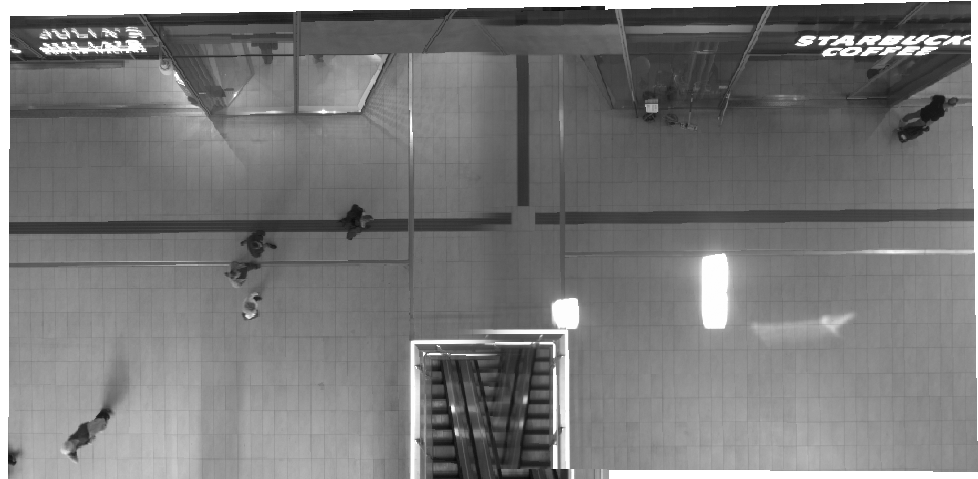
\includegraphics[width=0.4\textheight]{imgs/bg10.png}
\caption{Utrecht Centraal, cameras point of view (Floorfield 10)}
%\cite{bibliography}
\label{fig:trainf10}
\end{figure}


\paragraph{Sample from the dataset}
In this section are showed a few example of trajectories selected form the dataset.
Each trajectory is presented with three types of plot: the line of the path (L), the heatmap generated from that path (H) and the velocities distribution along $x$ and $y$ (V).
A great number of collected path are given by pedestrians that have walked from left to right or from right to left, along a \emph{semi}-straight horizontal line.
\\As first example: the (Figure \ref{fig:semi_straight1_L} - \ref{fig:semi_straight1_V}) is the path (1) of a random pedestrian that has walked almost straight all the way.
The interpretation of the (V) plot in (Figure \ref{fig:semi_straight1_V}) permit to know the direction of that pedestrian.
For (1) the velocity distribution is focalized in the negative velocity along $x$ and close to zero along $y$.
That means: the pedestrian goes from right to left along $x$.
The next path (2), in (Figure \ref{fig:semi_straight2_L} - \ref{fig:semi_straight2_V}) is pretty similar to the (1), but instead it proceed from left to right with positive velocity.
\\Other paths are like the one in (Figure \ref{fig:semi_straight_down_L} - \ref{fig:semi_straight_down_V}), path (3), and (Figure \ref{fig:semi_straight_up_L} - \ref{fig:semi_straight_up_V}), path (4).
Both path (3) and (4) go straight almost all the length of the field, then (3) turn down and (4) turn up to go exit the field.

\begin{figure}[ht]
\begin{minipage}[c]{0.35\linewidth}
\centering
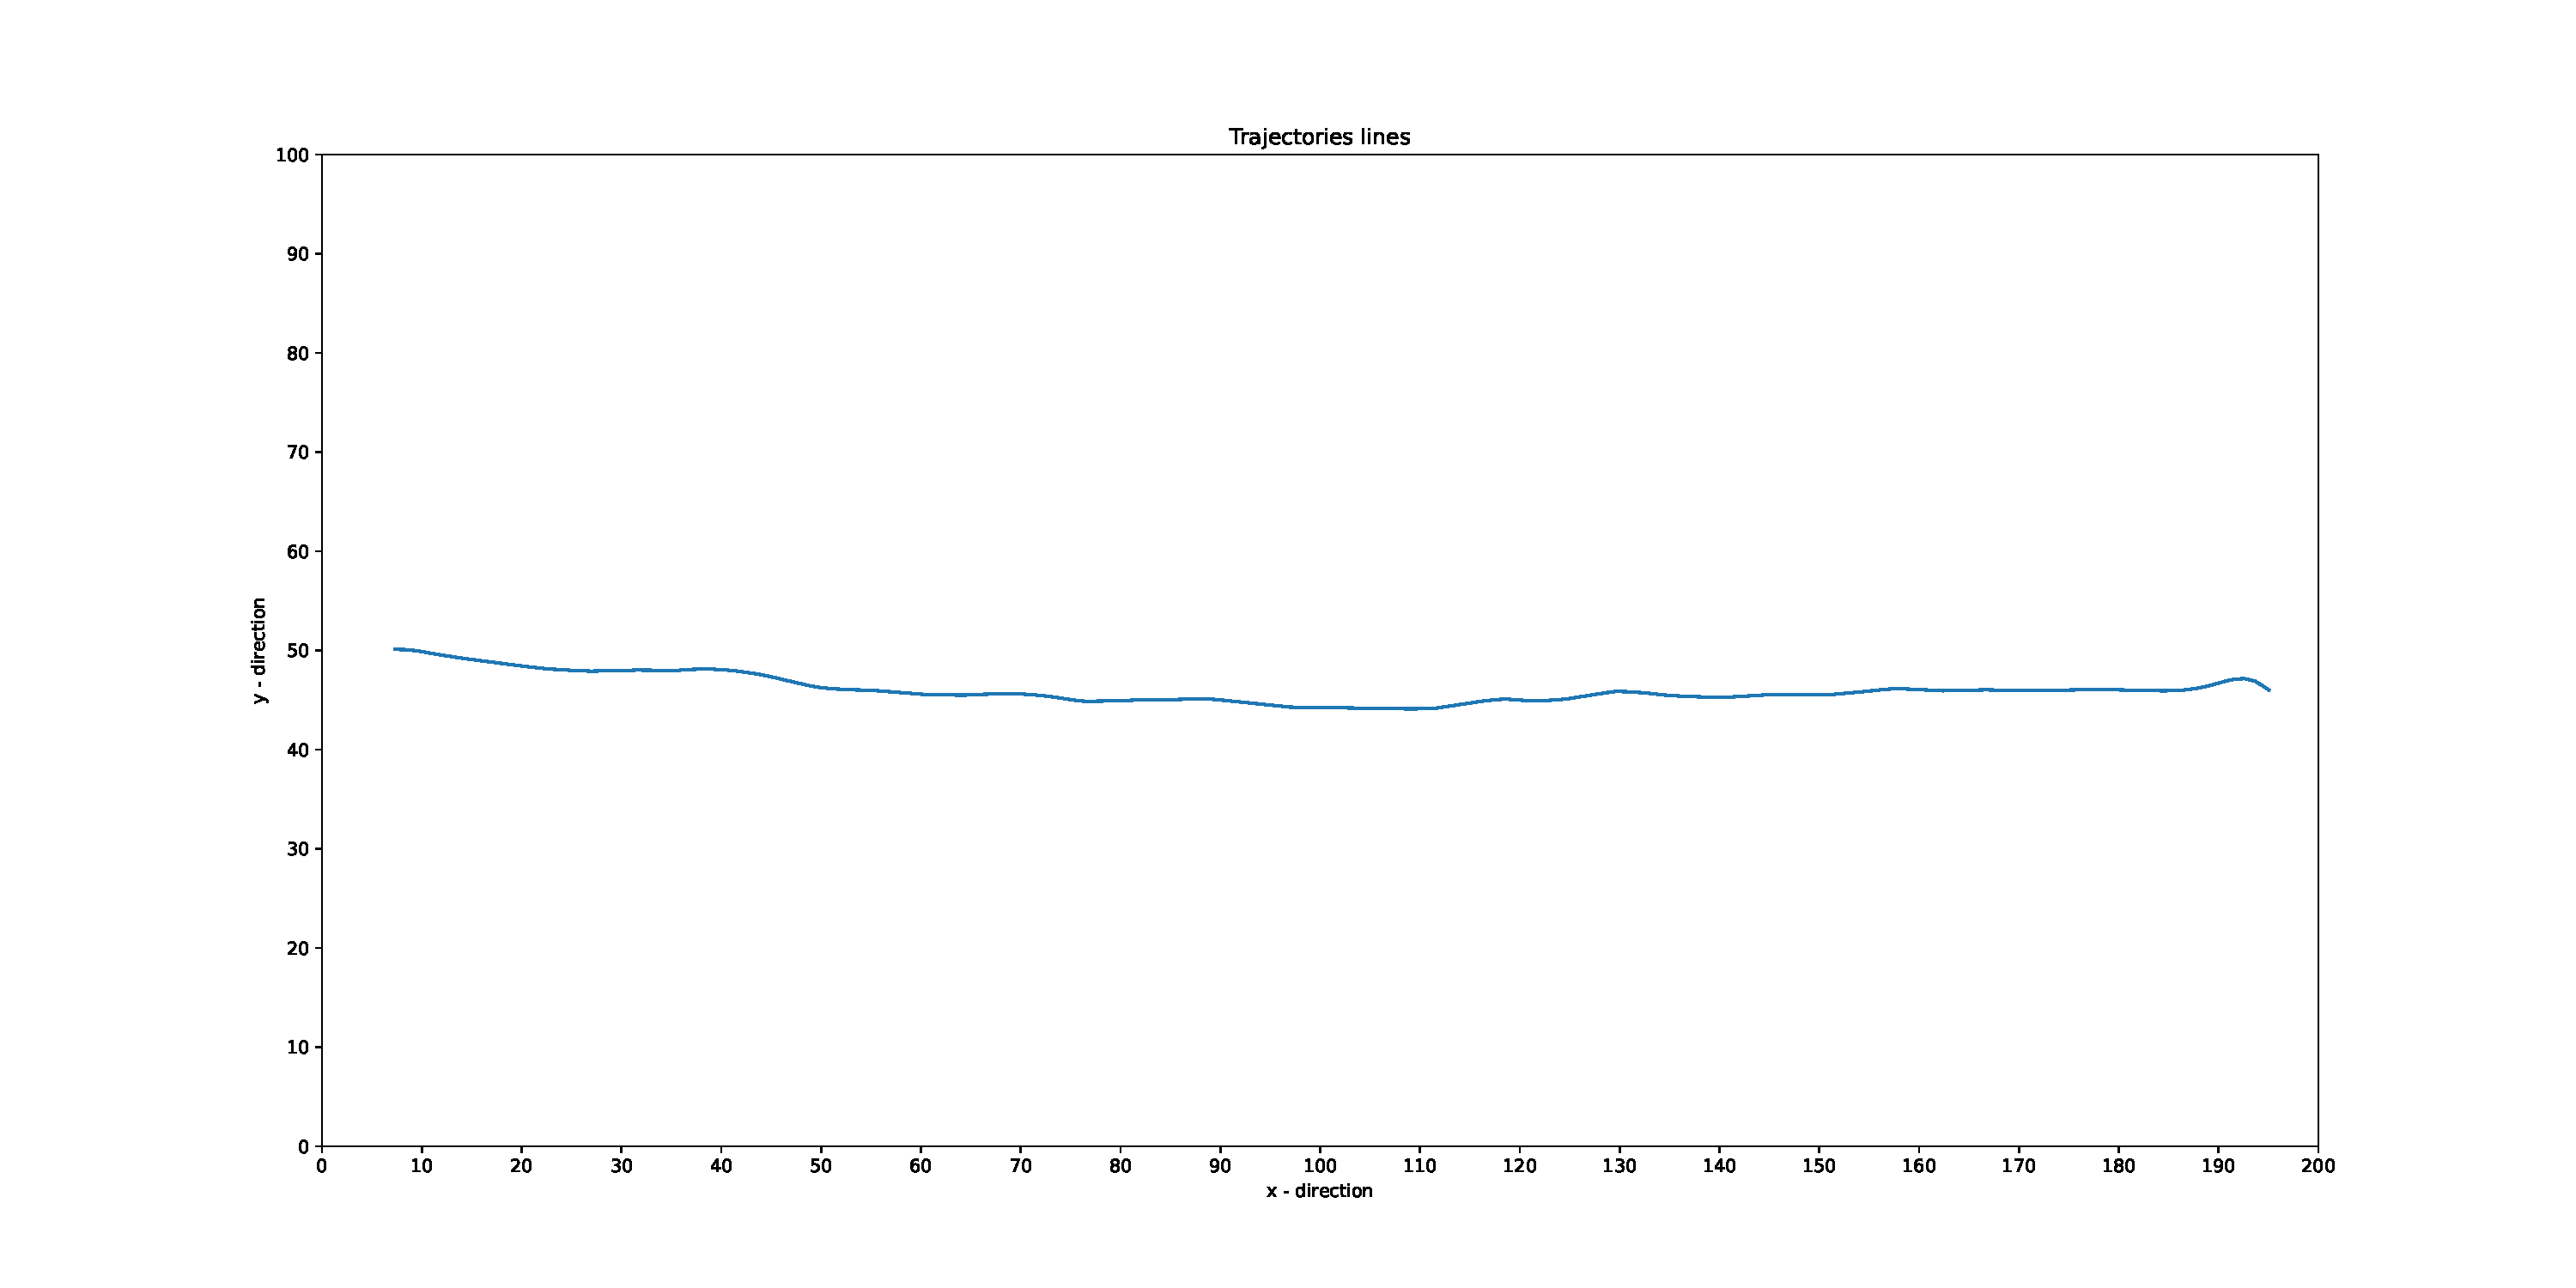
\includegraphics[ width=1\textwidth]{fig/belle_traiettorie/nice selection/figure_trainf10_RealData_lines_19marzo_select_single_NP_19_13108495}
\captionsetup{width=.8\linewidth}
\caption{Plot L, path 1}
\label{fig:semi_straight1_L}
\end{minipage}
\begin{minipage}[c]{0.35\linewidth}
\centering
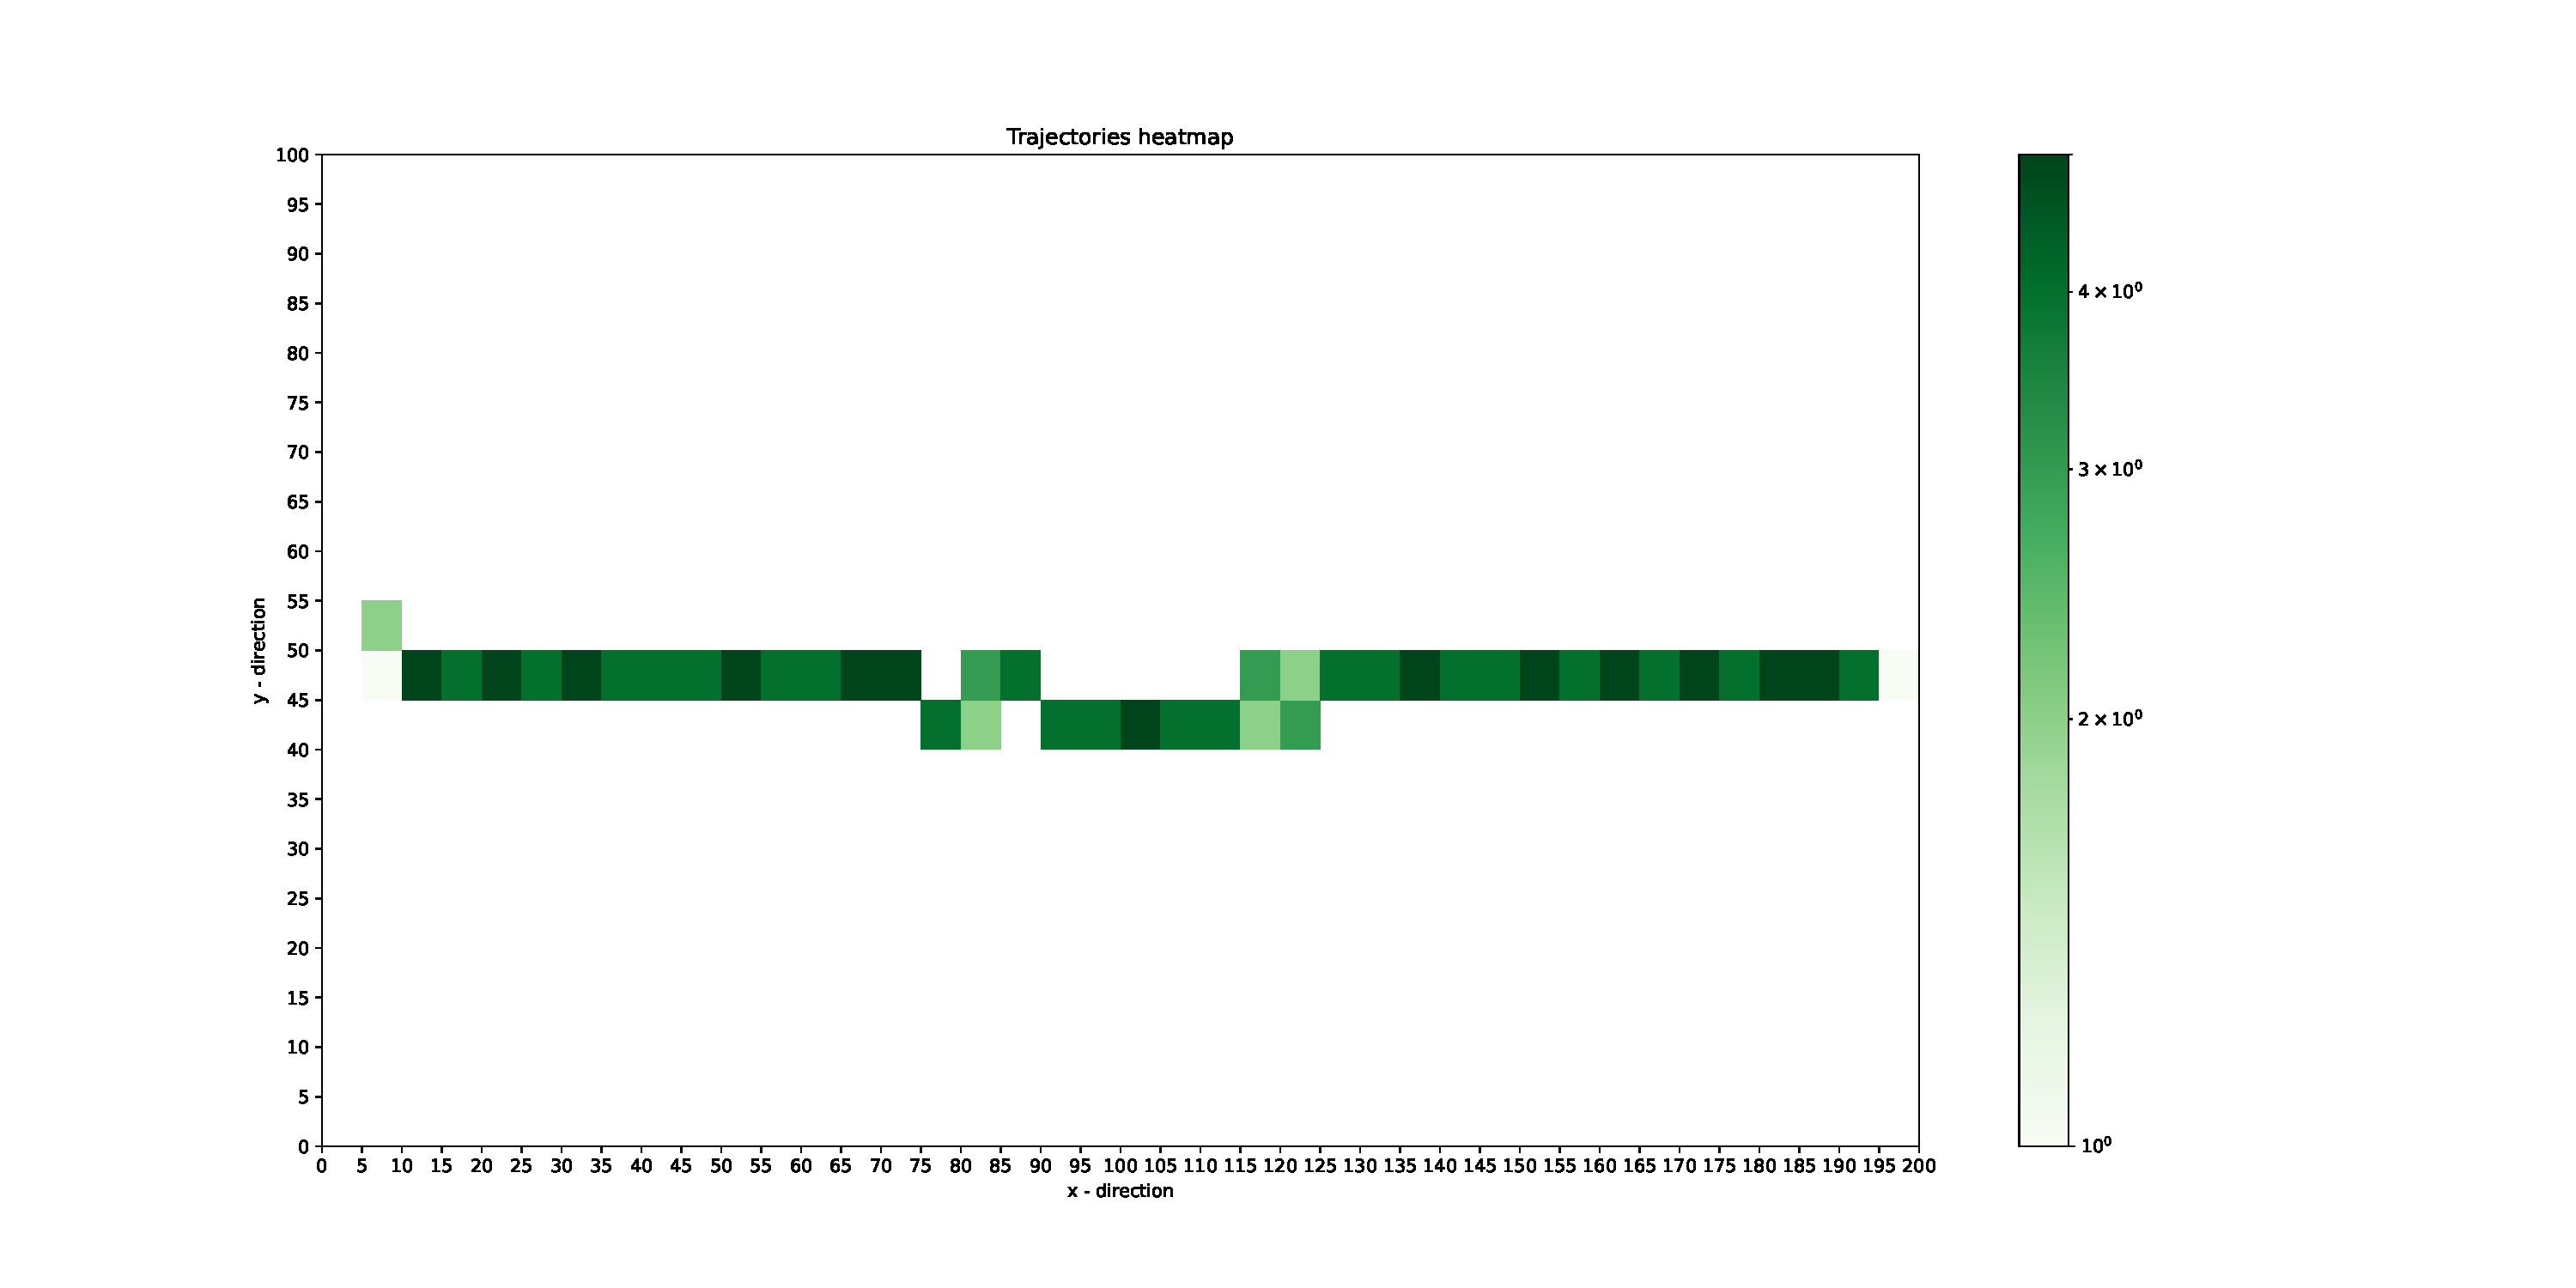
\includegraphics[ width=1\textwidth]{fig/belle_traiettorie/nice selection/figure_trainf10_RealData_heatmap_19marzo_select_single_NP_19_13108495}
\captionsetup{width=.8\linewidth}
\caption{Plot H, path 1}
\label{fig:semi_straight1_H}
\end{minipage}
\begin{minipage}[c]{0.25\linewidth}
\centering
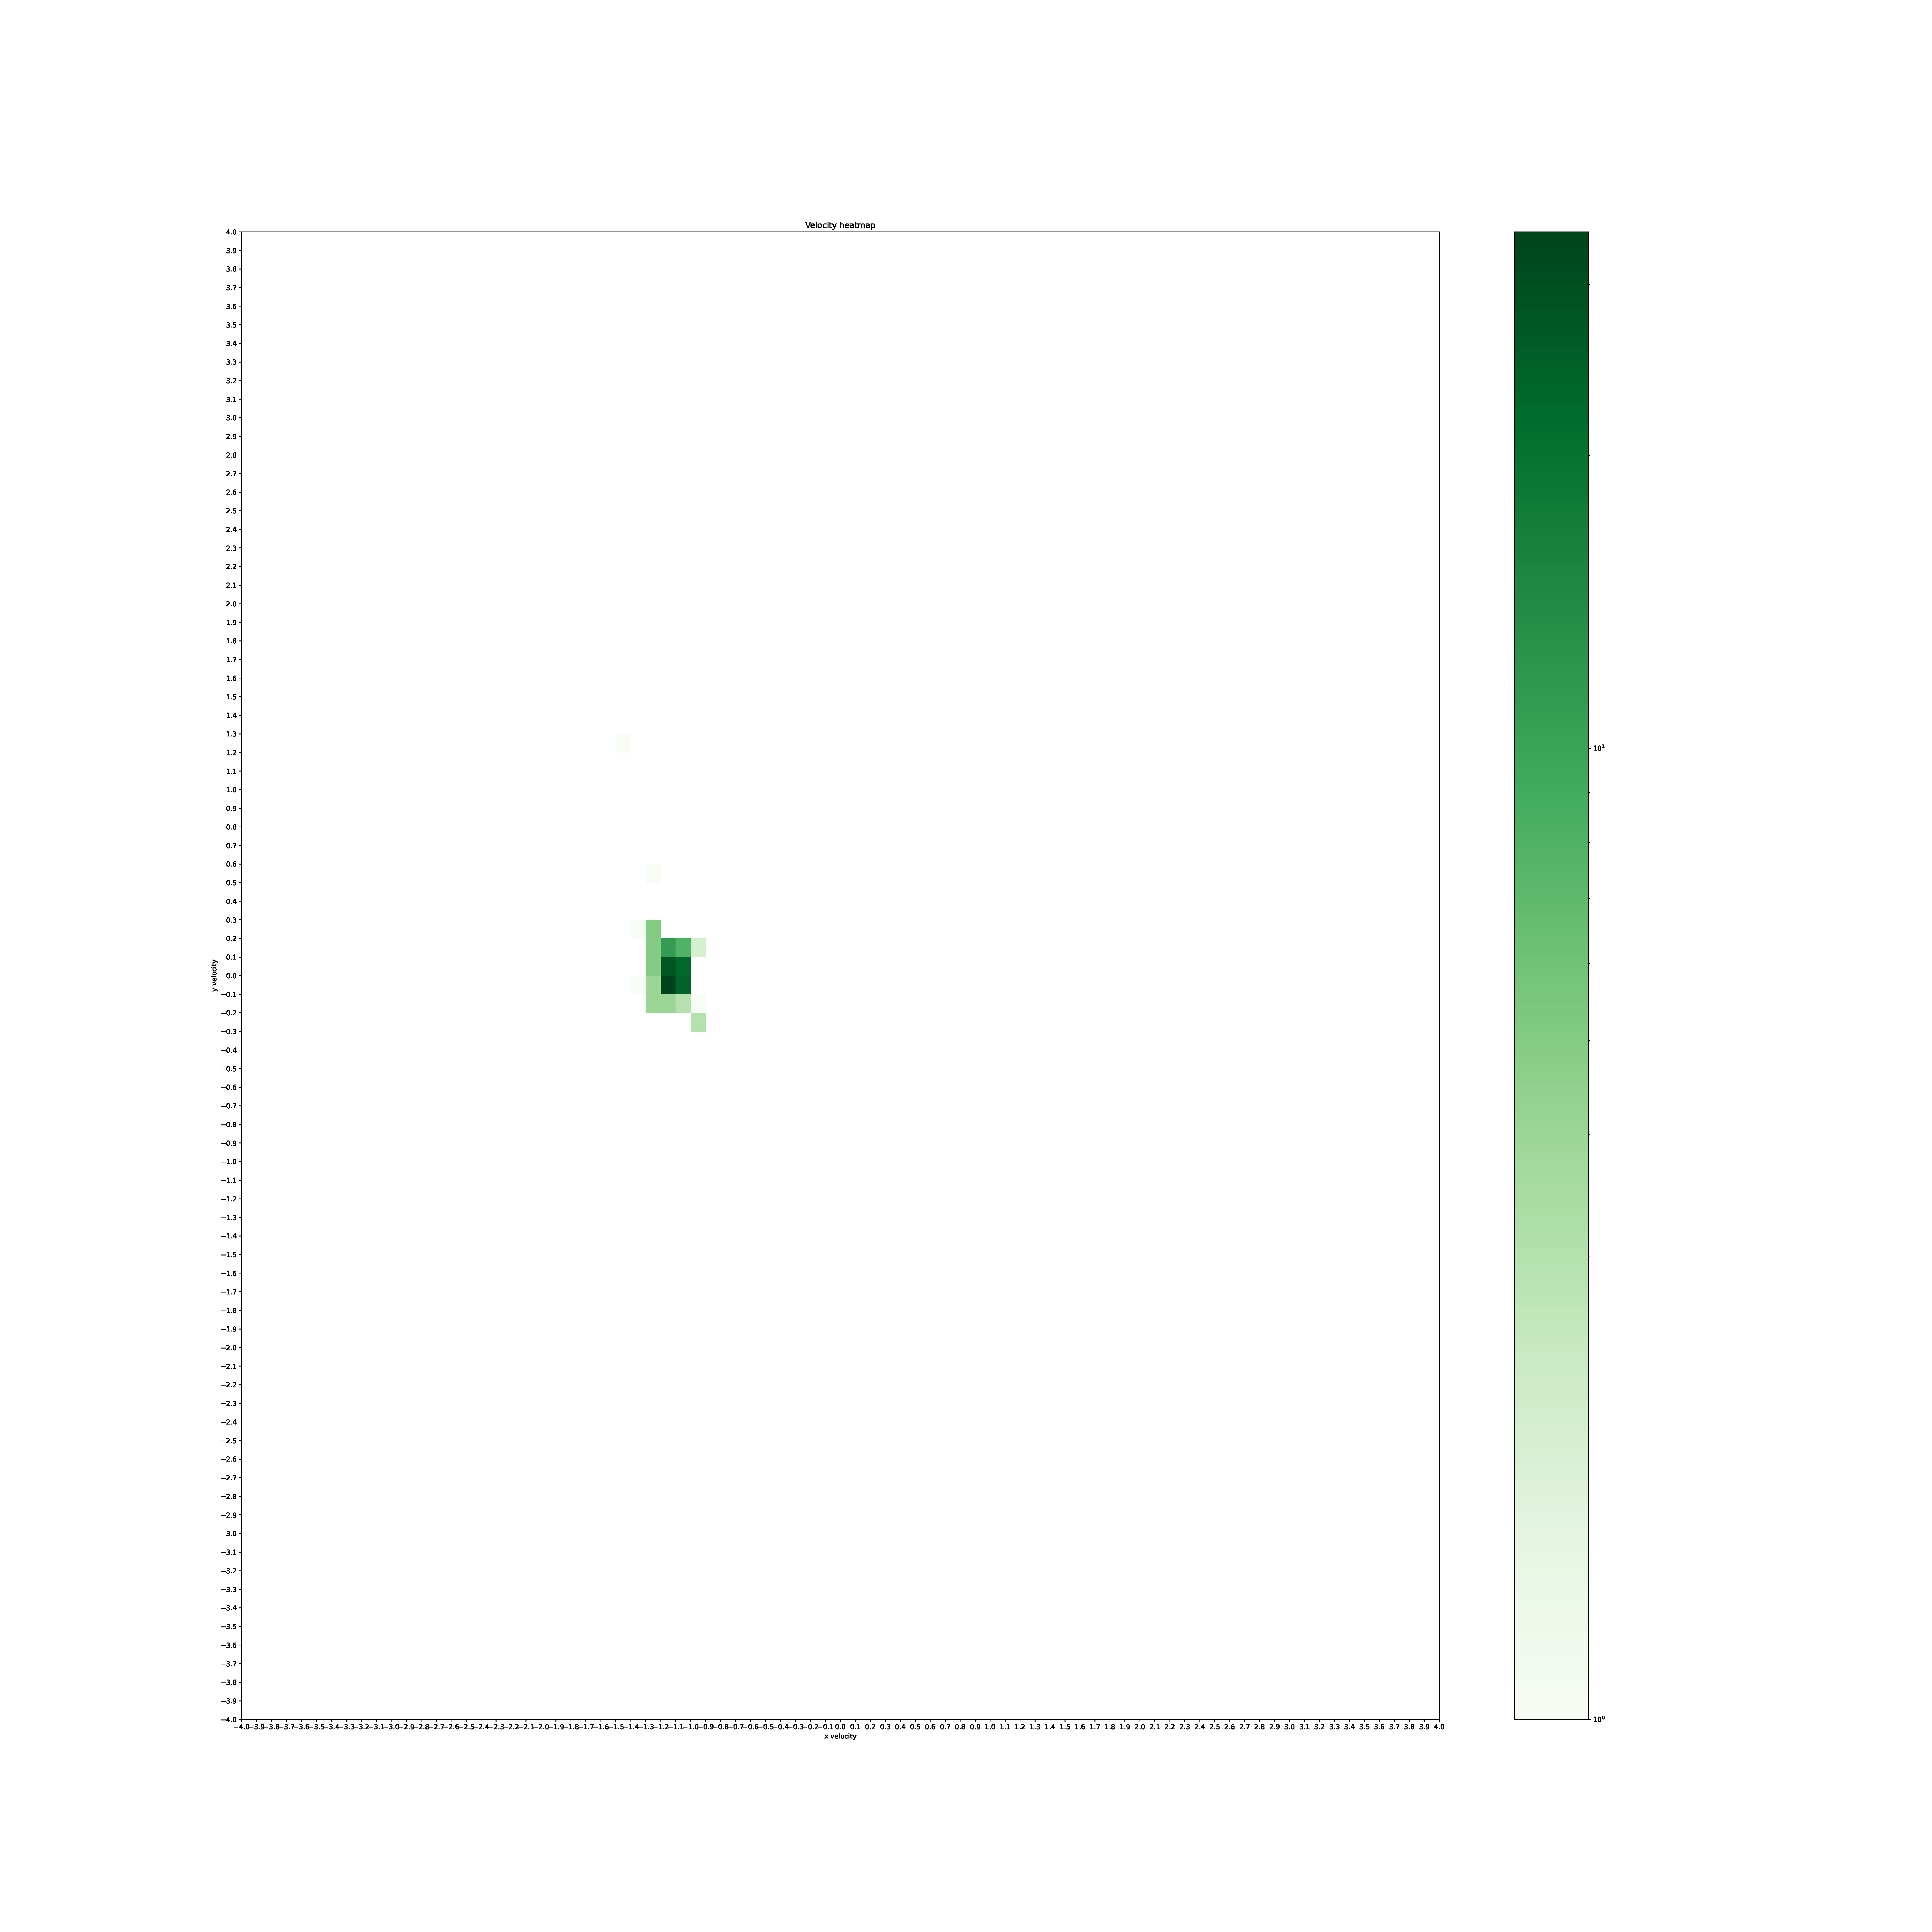
\includegraphics[ width=0.9\textwidth]{fig/belle_traiettorie/nice selection/figure_trainf10_RealData_velocity_heatmap_19marzo_select_single_NP_19_13108495}
\captionsetup{width=.8\linewidth}
\caption{Plot V, path 1}
\label{fig:semi_straight1_V}
\end{minipage}
\end{figure}
% --- --- --- --- --- --- --- --- --- --- --- --- --- --- --- --- --- --- --- --- --- --- --- --- --- --- --- --- ---
\begin{figure}[ht]
\begin{minipage}[c]{0.35\linewidth}
\centering
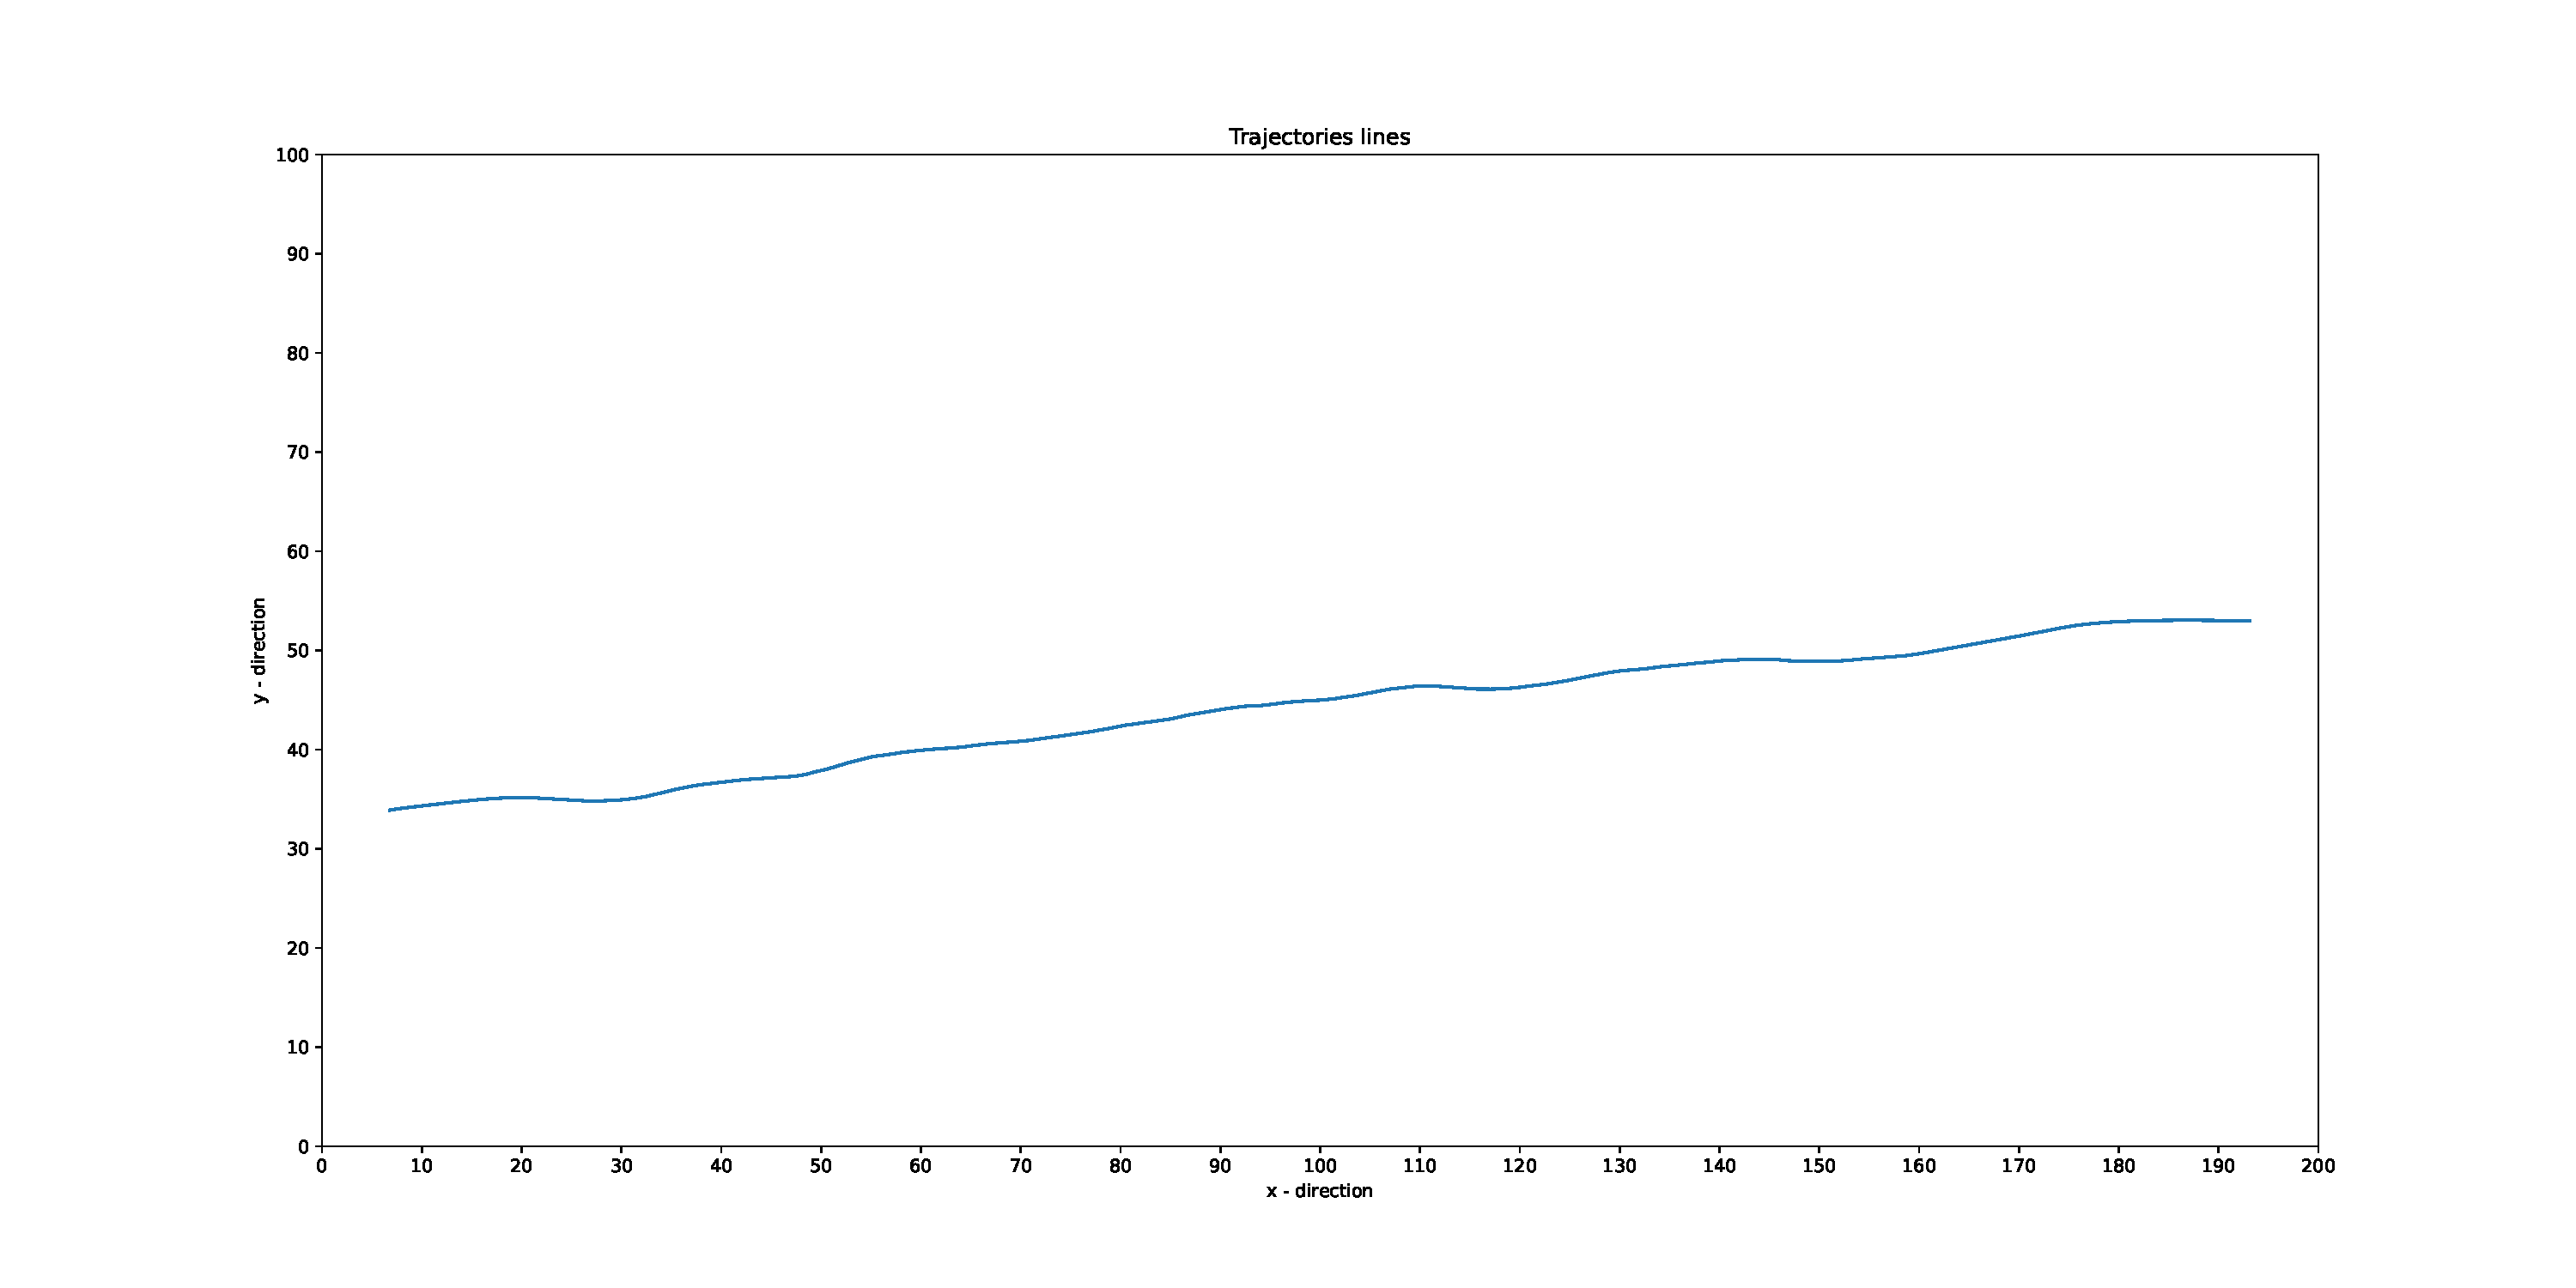
\includegraphics[ width=1\textwidth]{fig/belle_traiettorie/nice selection/figure_trainf10_RealData_lines_19marzo_select_single_NP_19_13074453}
\captionsetup{width=.8\linewidth}
\caption{Plot L, path 2}
\label{fig:semi_straight2_L}
\end{minipage}
\begin{minipage}[c]{0.35\linewidth}
\centering
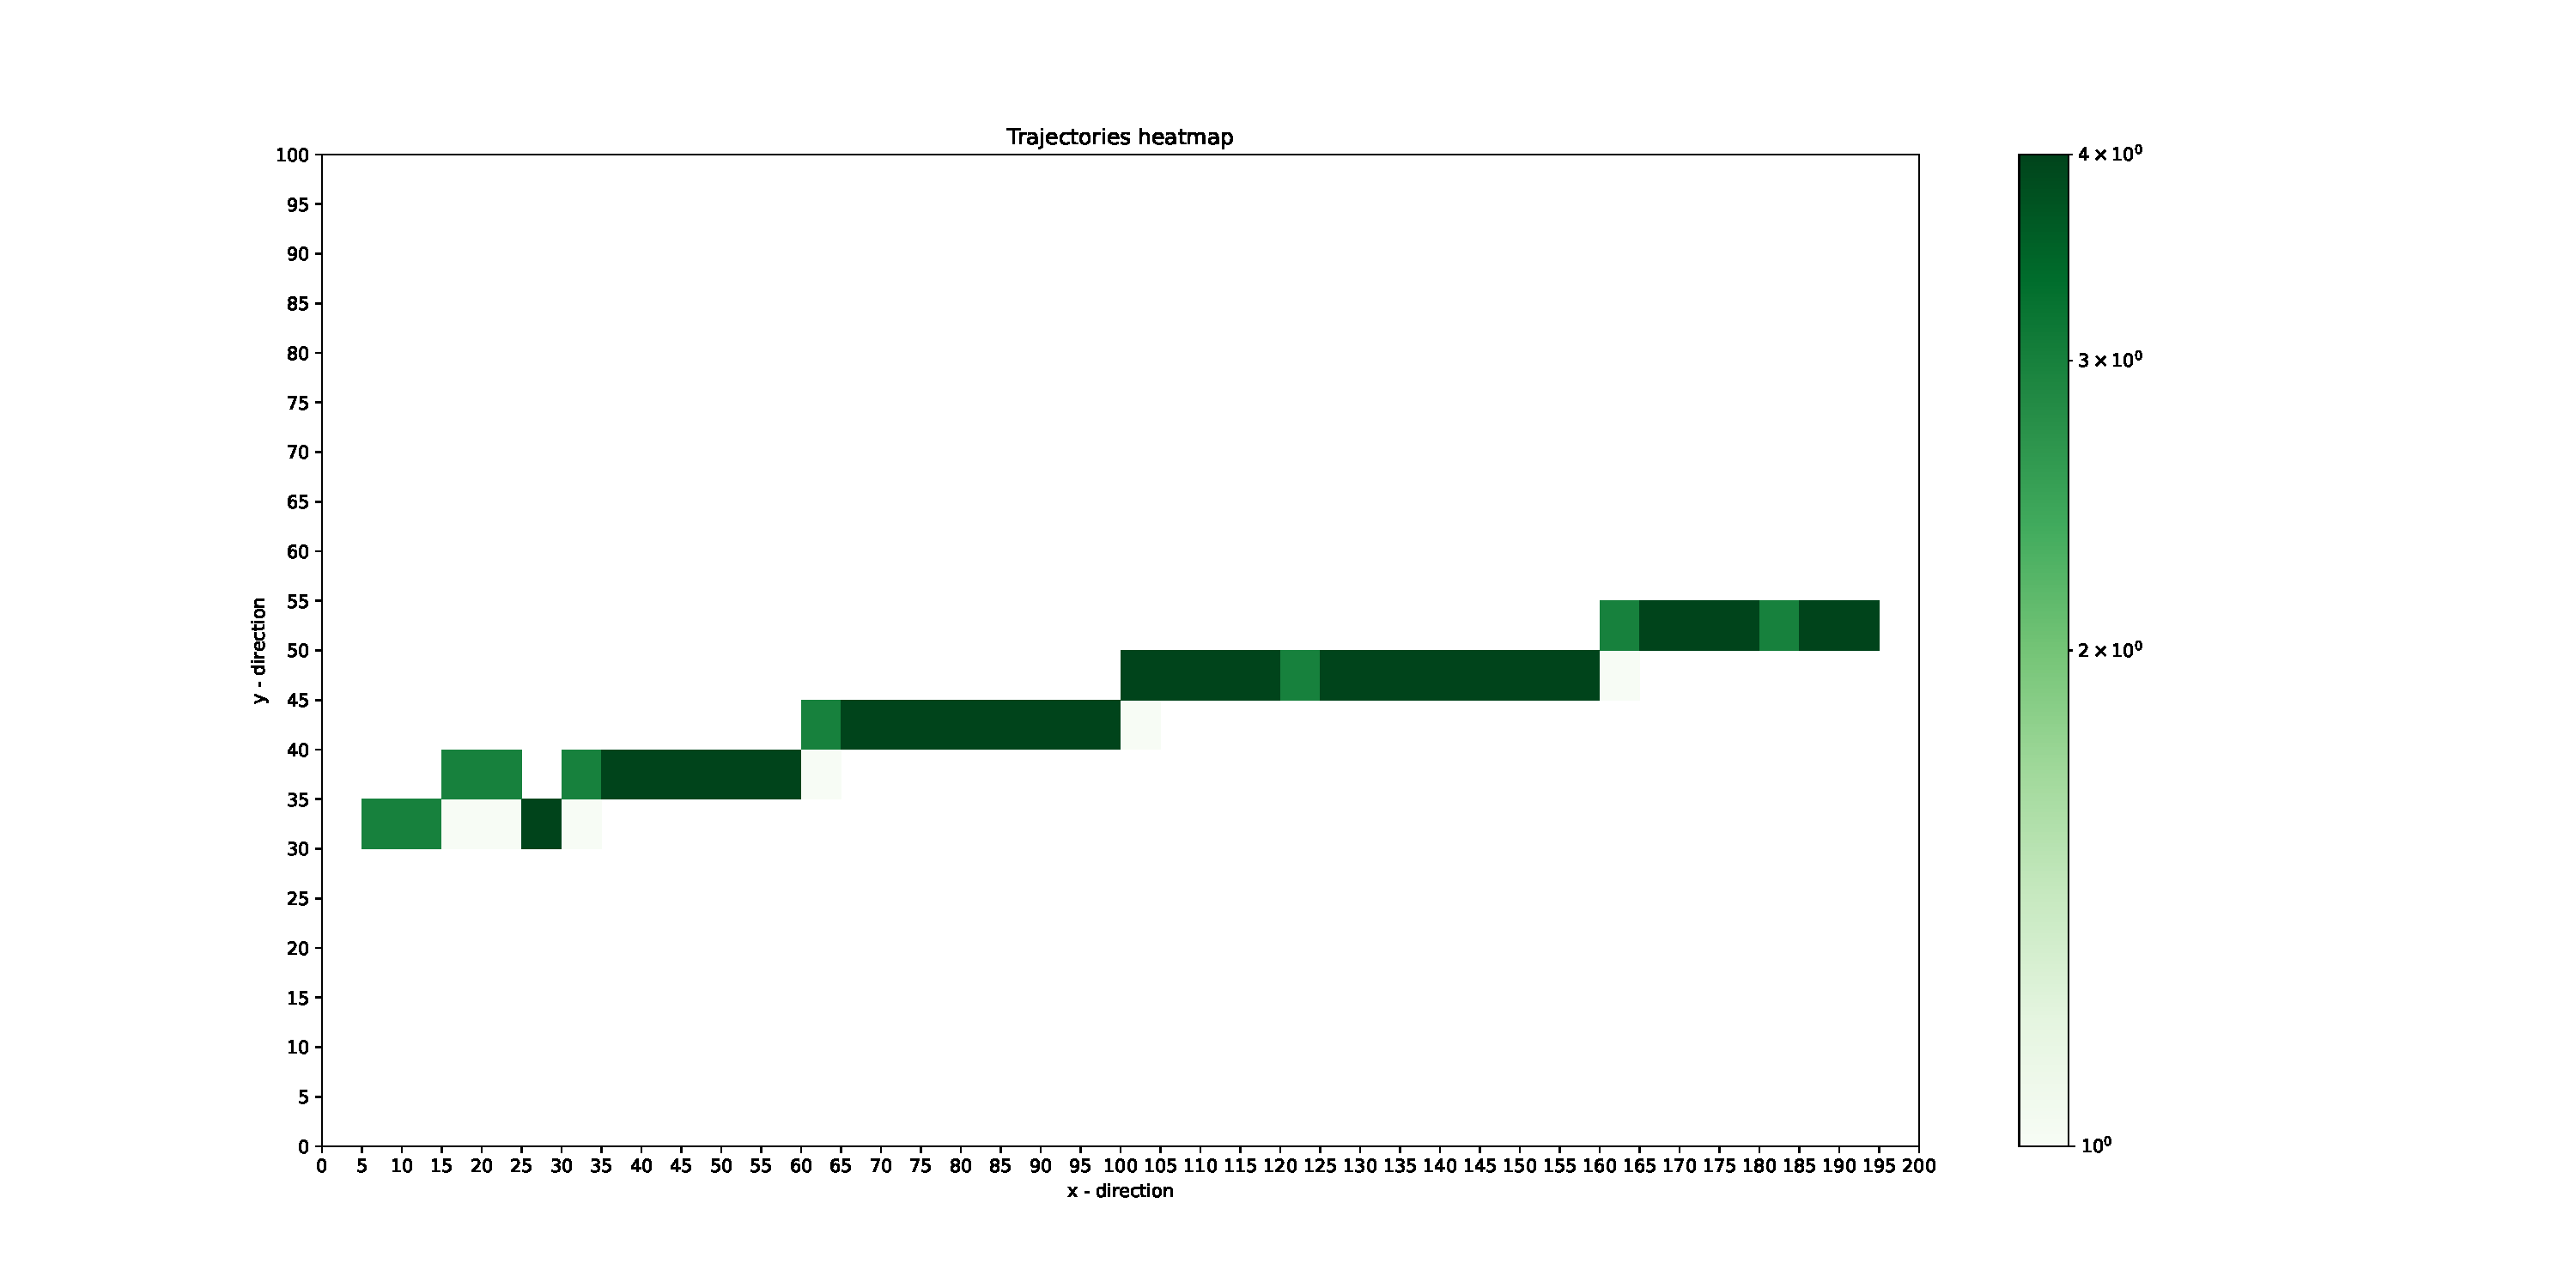
\includegraphics[ width=1\textwidth]{fig/belle_traiettorie/nice selection/figure_trainf10_RealData_heatmap_19marzo_select_single_NP_19_13074453}
\captionsetup{width=.8\linewidth}
\caption{Plot H, path 2}
\label{fig:semi_straight2_H}
\end{minipage}
\begin{minipage}[c]{0.25\linewidth}
\centering
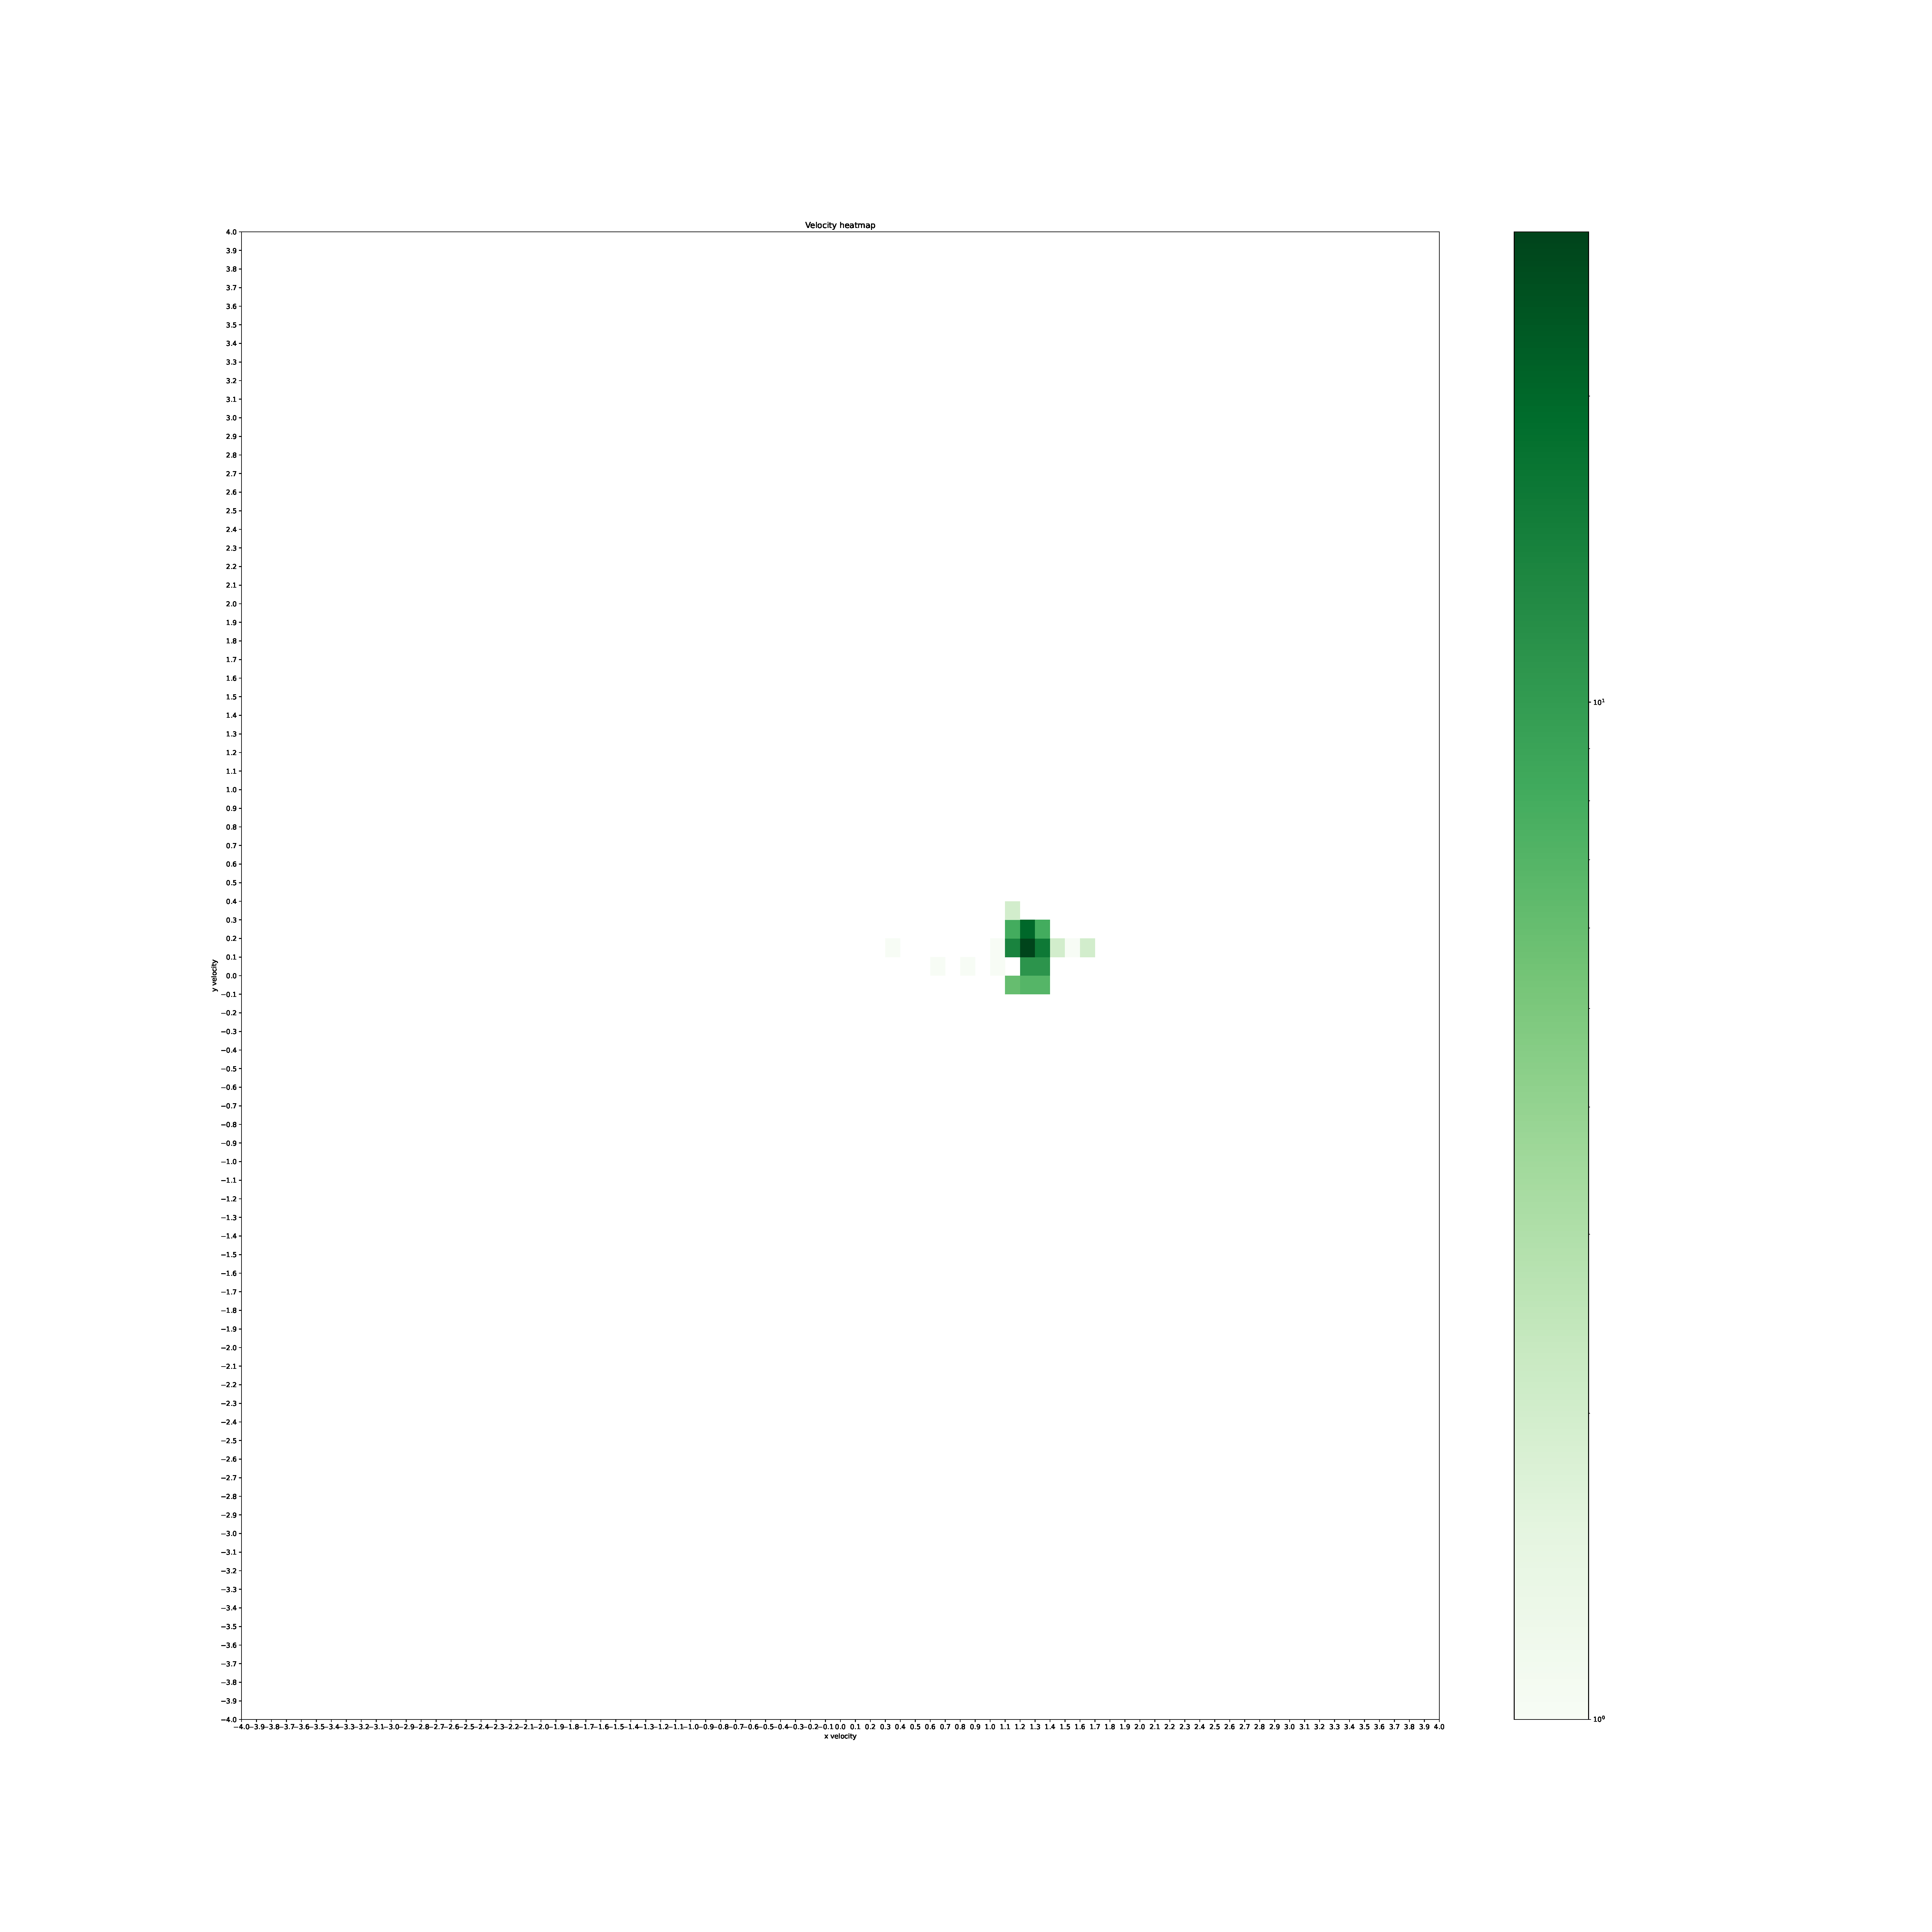
\includegraphics[ width=0.9\textwidth]{fig/belle_traiettorie/nice selection/figure_trainf10_RealData_velocity_heatmap_19marzo_select_single_NP_19_13074453}
\captionsetup{width=.8\linewidth}
\caption{Plot V, path 2}
\label{fig:semi_straight2_V}
\end{minipage}
\end{figure}
% --- --- --- --- --- --- --- --- --- --- --- --- --- --- --- --- --- --- --- --- --- --- --- --- --- --- --- --- ---
\begin{figure}[ht]
\begin{minipage}[c]{0.35\linewidth}
\centering
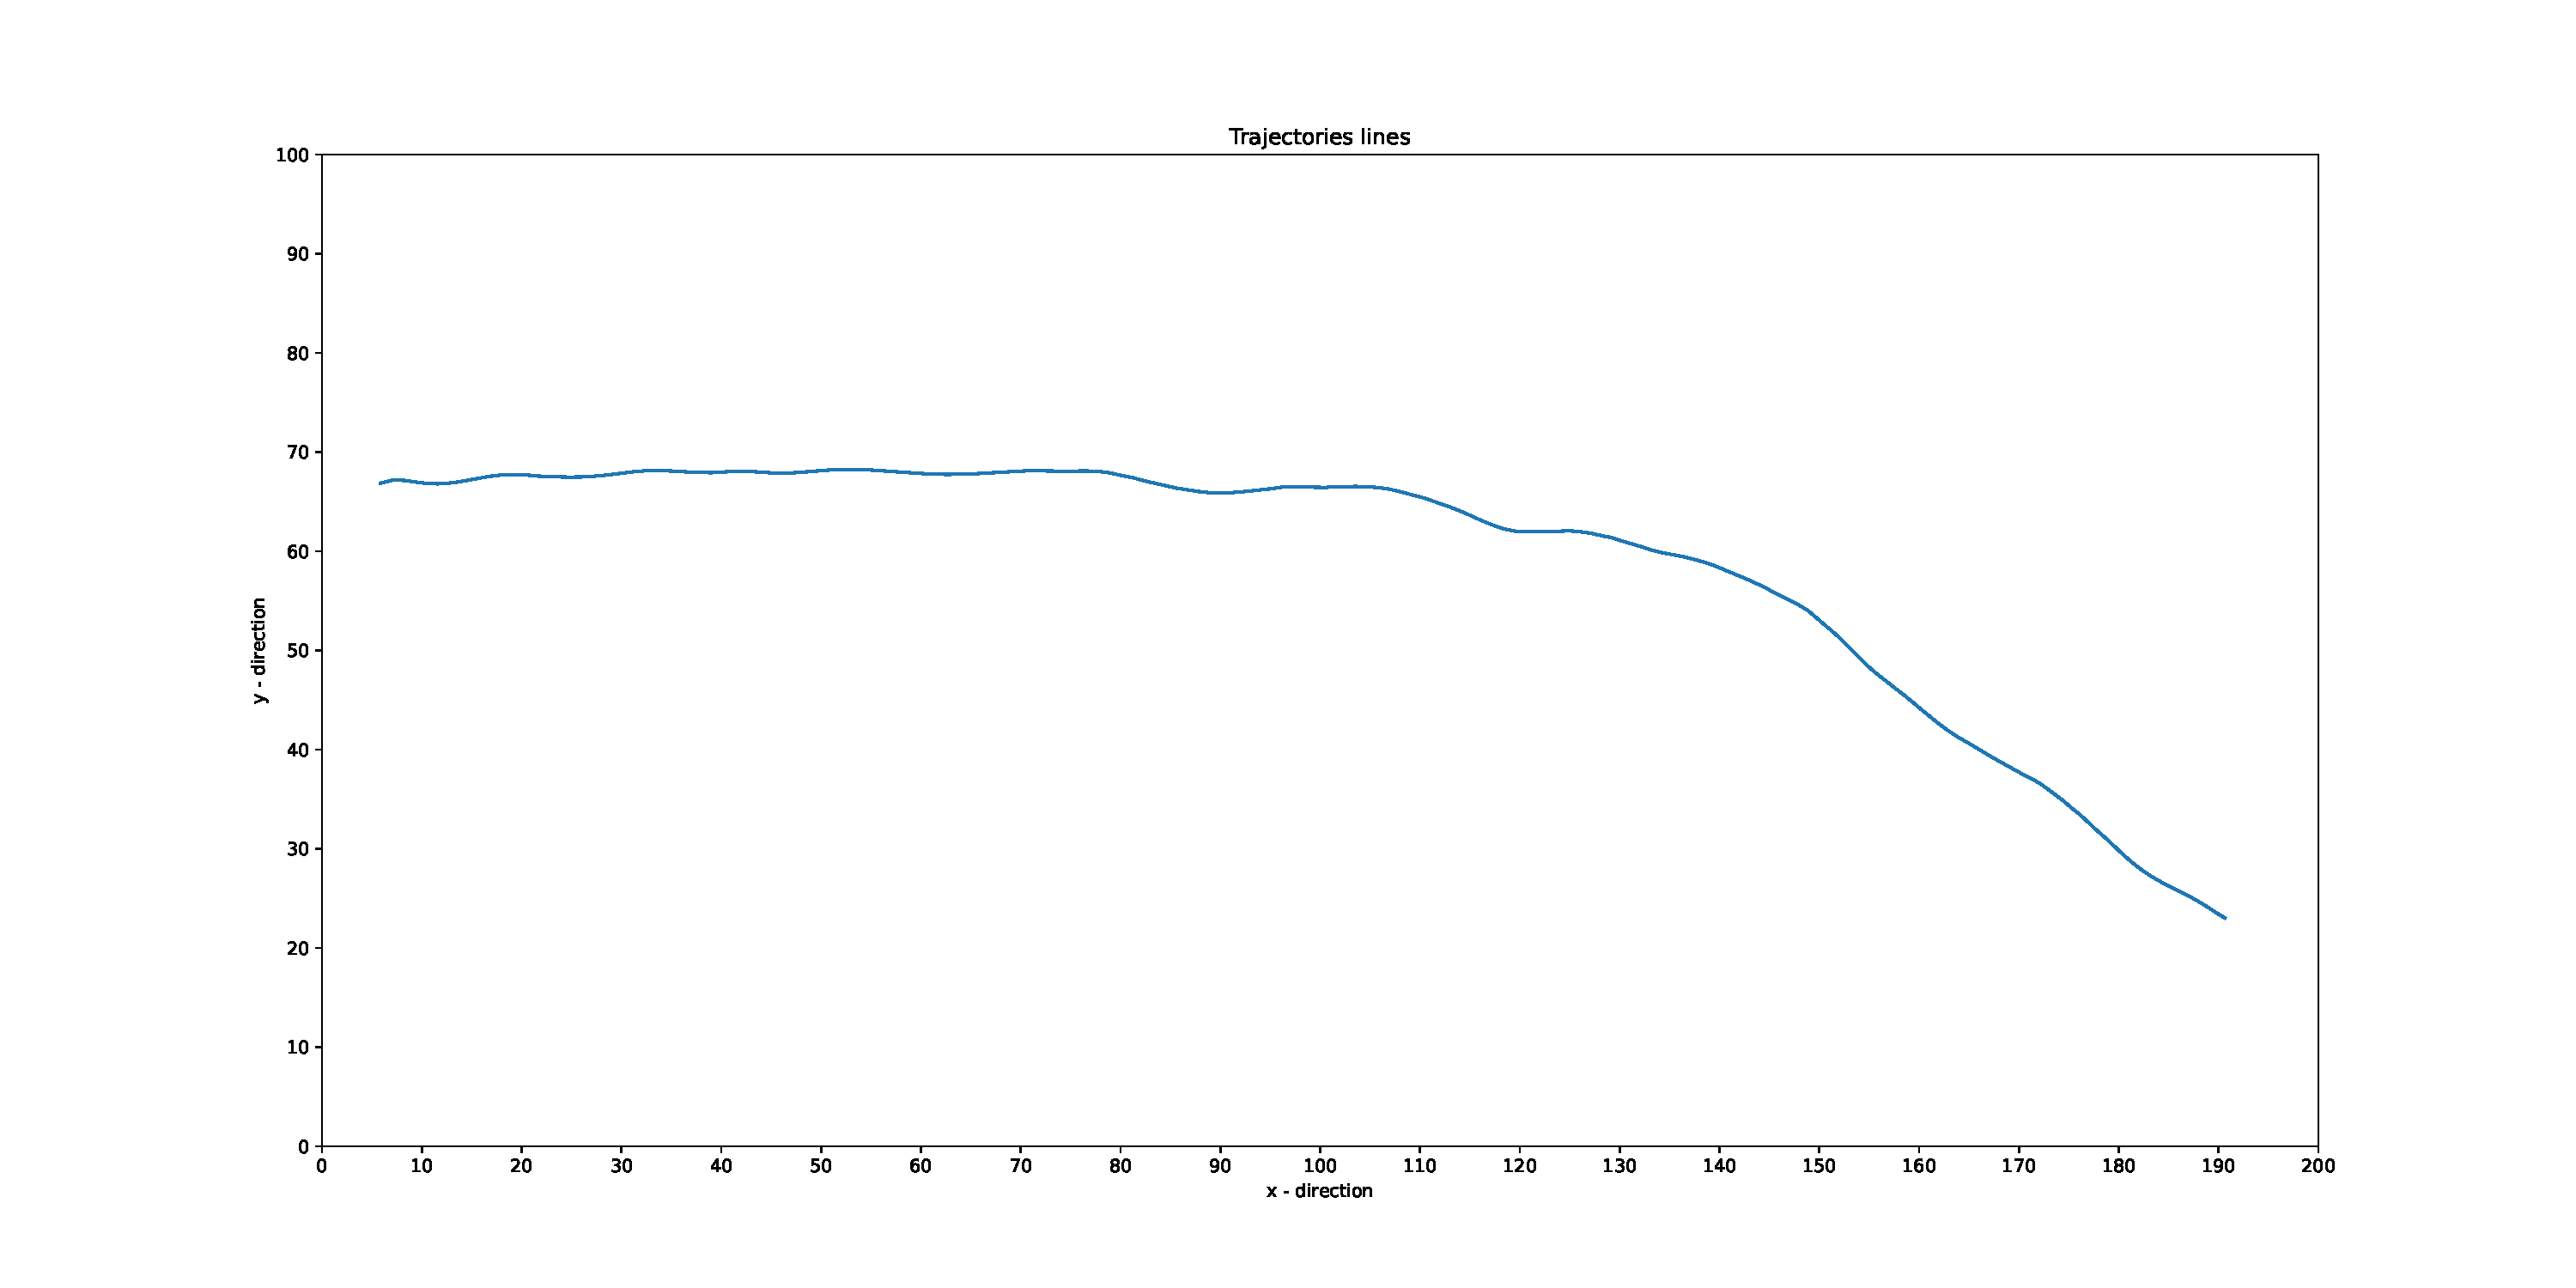
\includegraphics[ width=1\textwidth]{fig/belle_traiettorie/nice selection/figure_trainf10_RealData_lines_19marzo_select_single_NP_19_13108498}
\captionsetup{width=.8\linewidth}
\caption{Plot L, path 3}
\label{fig:semi_straight_down_L}
\end{minipage}
\begin{minipage}[c]{0.35\linewidth}
\centering
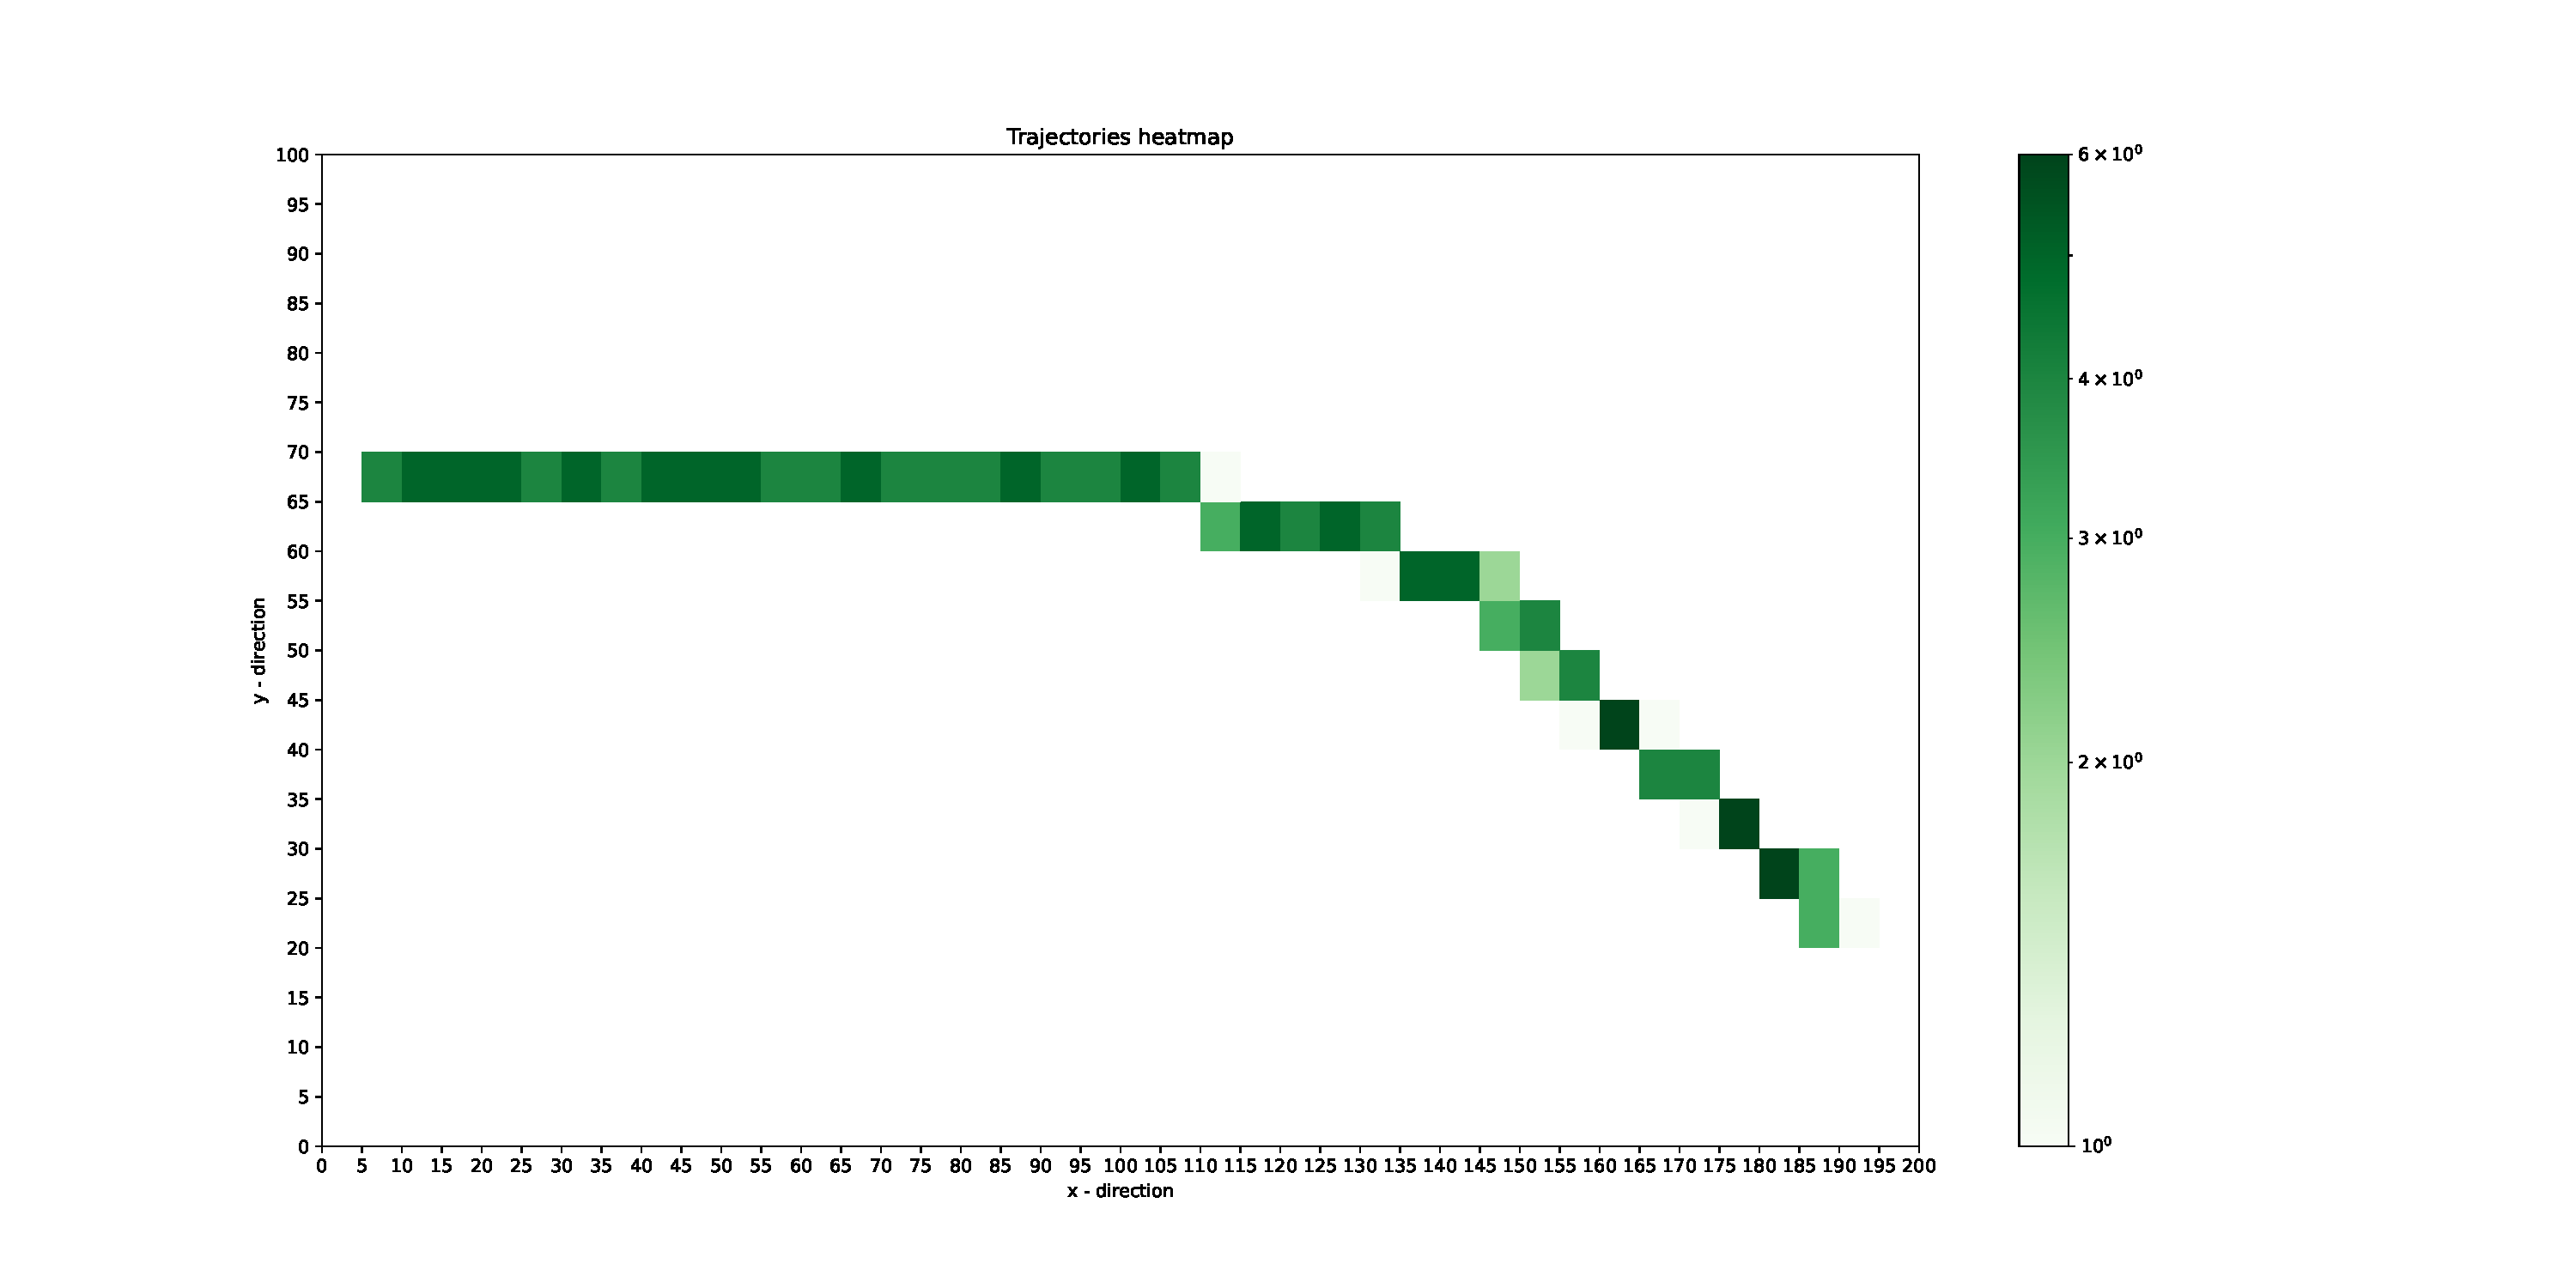
\includegraphics[ width=1\textwidth]{fig/belle_traiettorie/nice selection/figure_trainf10_RealData_heatmap_19marzo_select_single_NP_19_13108498}
\captionsetup{width=.8\linewidth}
\caption{Plot H, path 3}
\label{fig:semi_straight_down_H}
\end{minipage}
\begin{minipage}[c]{0.25\linewidth}
\centering
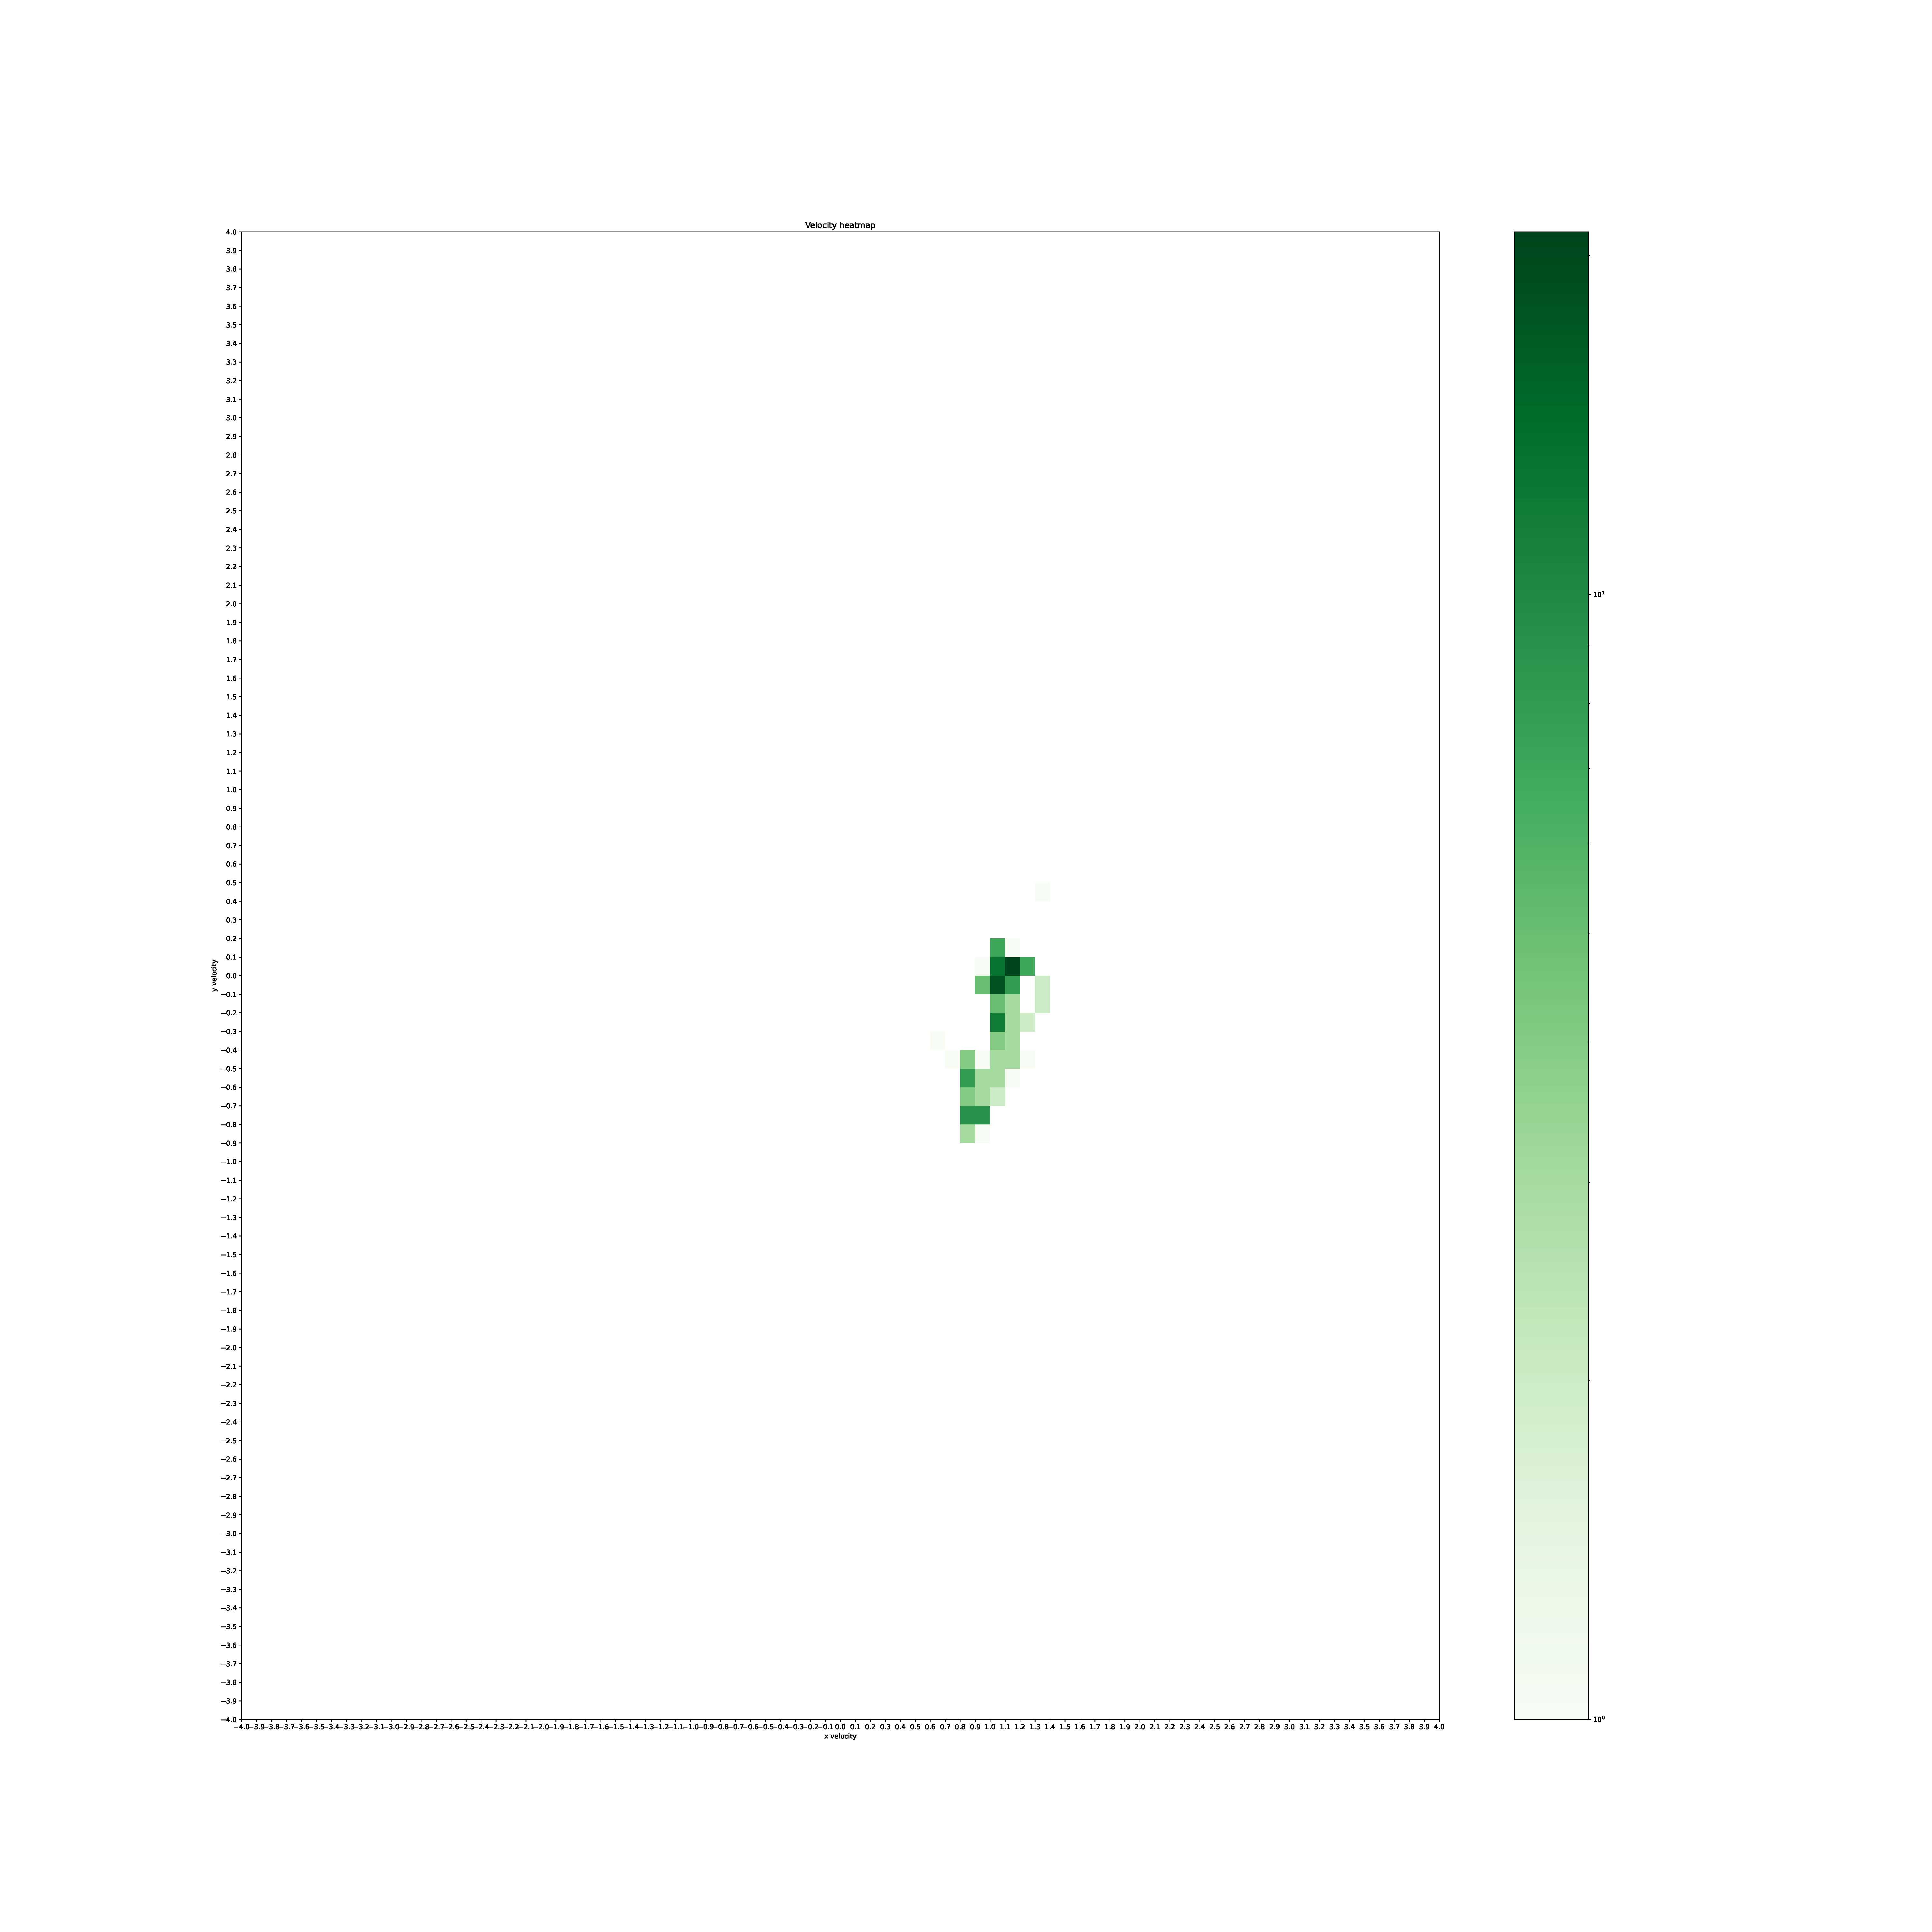
\includegraphics[ width=0.9\textwidth]{fig/belle_traiettorie/nice selection/figure_trainf10_RealData_velocity_heatmap_19marzo_select_single_NP_19_13108498}
\captionsetup{width=.8\linewidth}
\caption{Plot V, path 3}
\label{fig:semi_straight_down_V}
\end{minipage}
\end{figure}
% --- --- --- --- --- --- --- --- --- --- --- --- --- --- --- --- --- --- --- --- --- --- --- --- --- --- --- --- ---
\begin{figure}[ht]
\begin{minipage}[c]{0.35\linewidth}
\centering
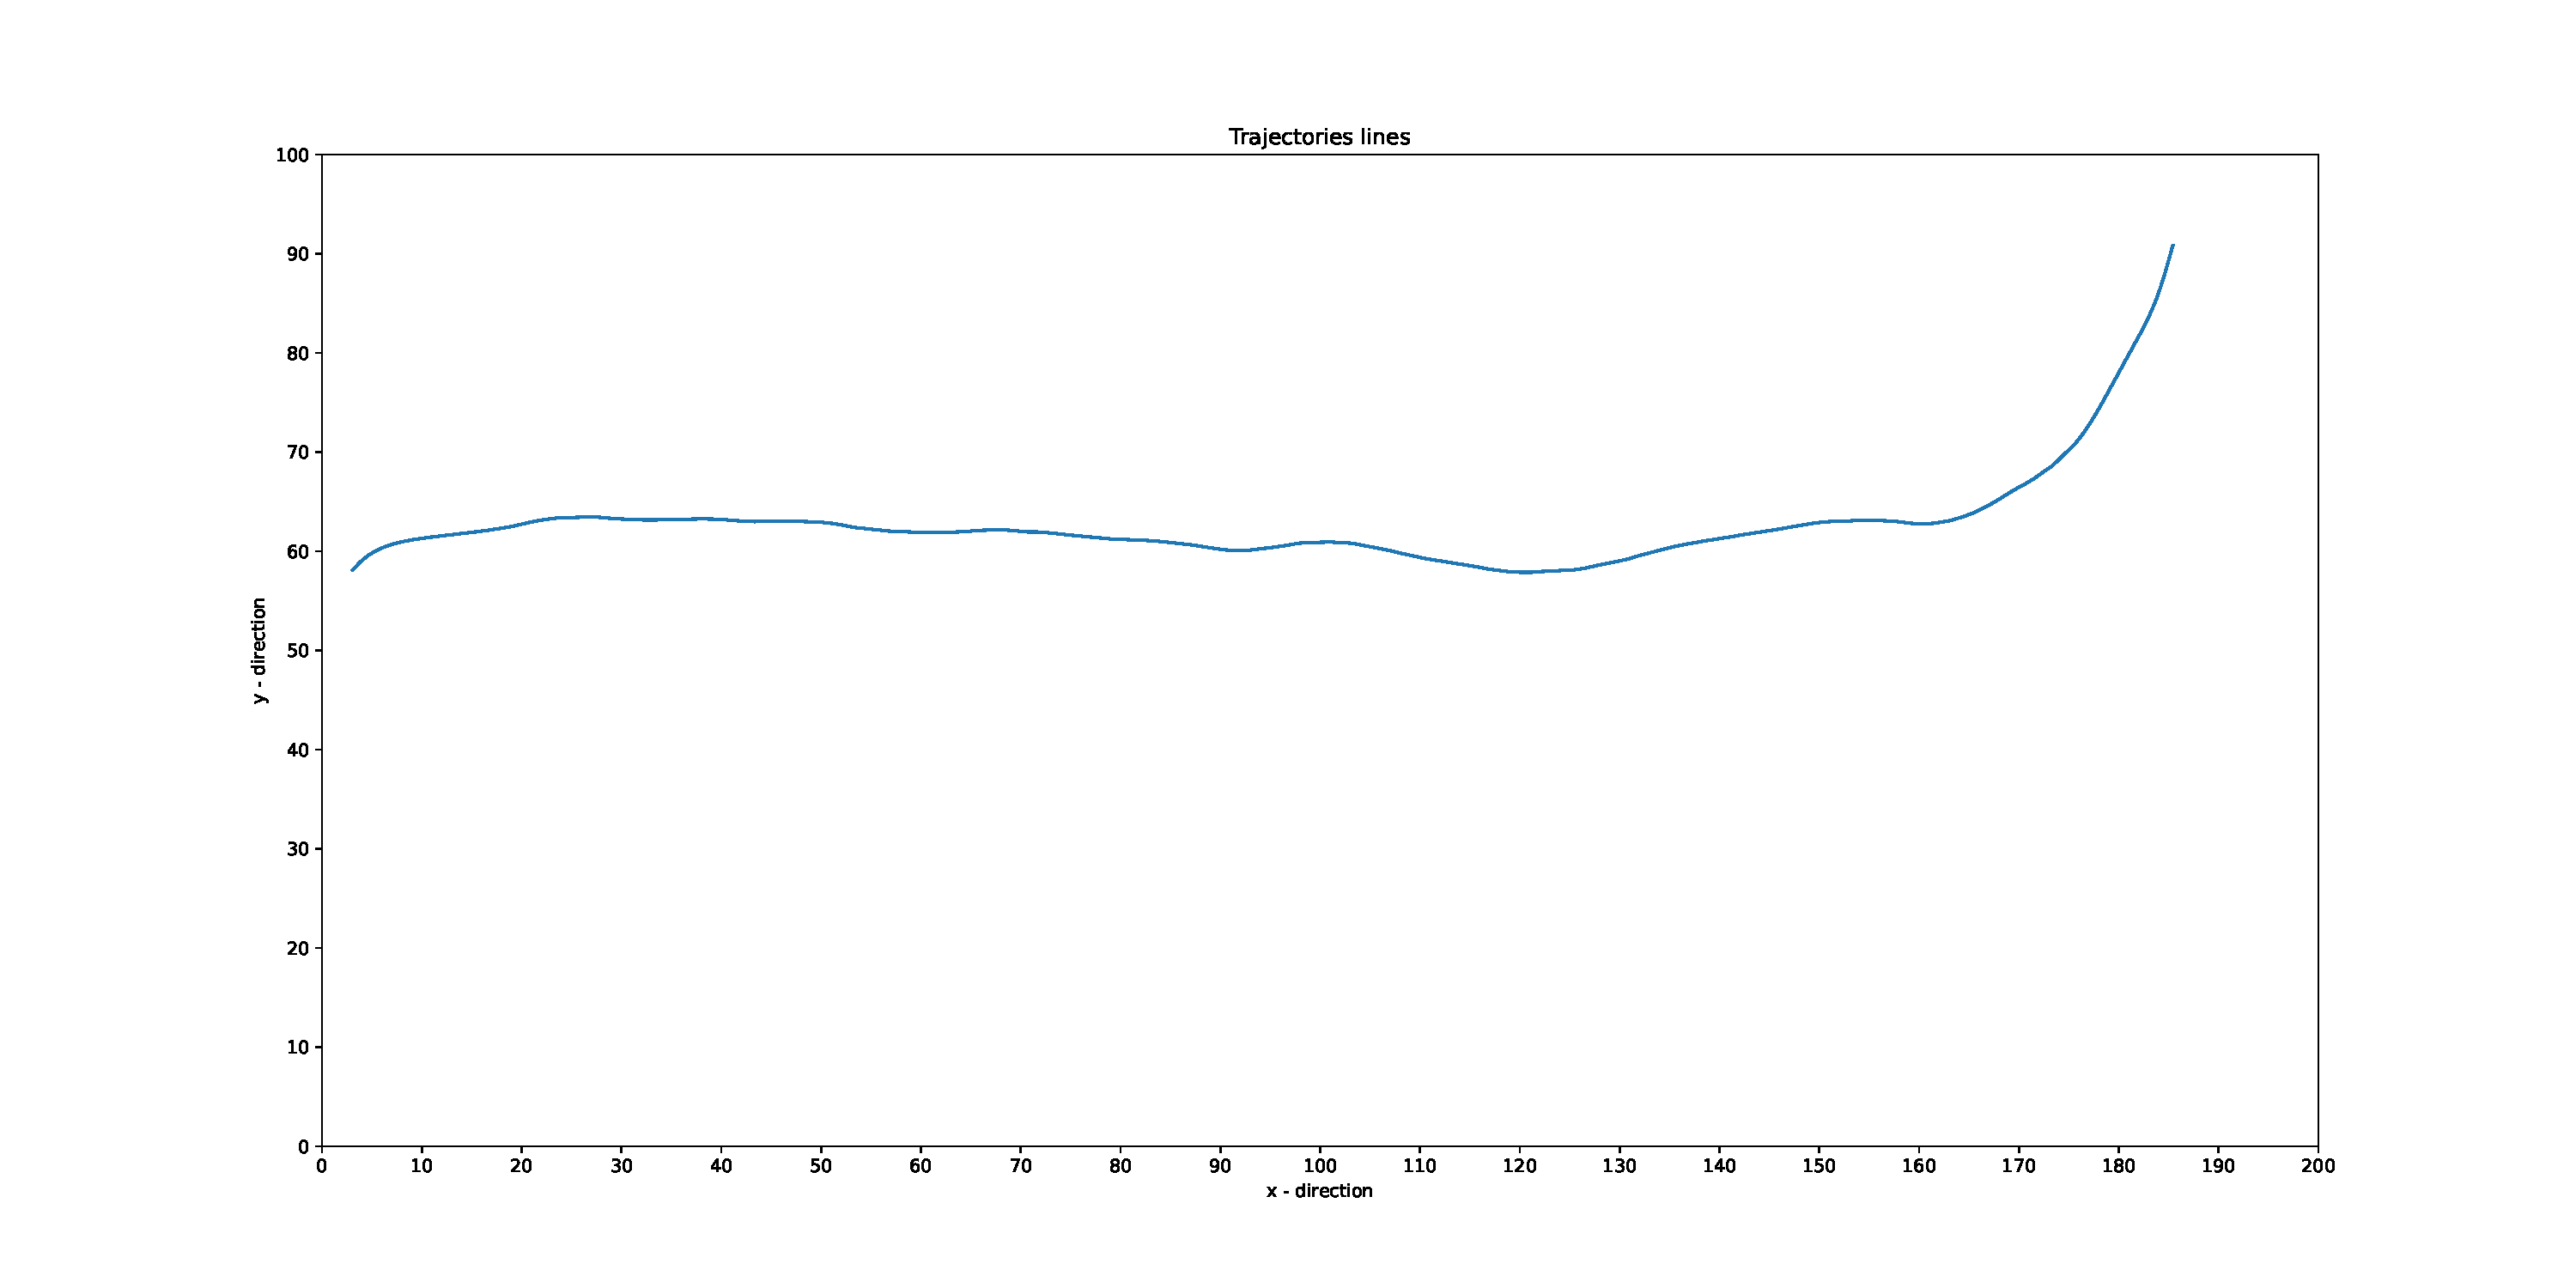
\includegraphics[ width=1\textwidth]{fig/belle_traiettorie/nice selection/figure_trainf10_RealData_lines_19marzo_select_single_NP_19_13140176}
\captionsetup{width=.8\linewidth}
\caption{Plot L, path 4}
\label{fig:semi_straight_up_L}
\end{minipage}
\begin{minipage}[c]{0.35\linewidth}
\centering
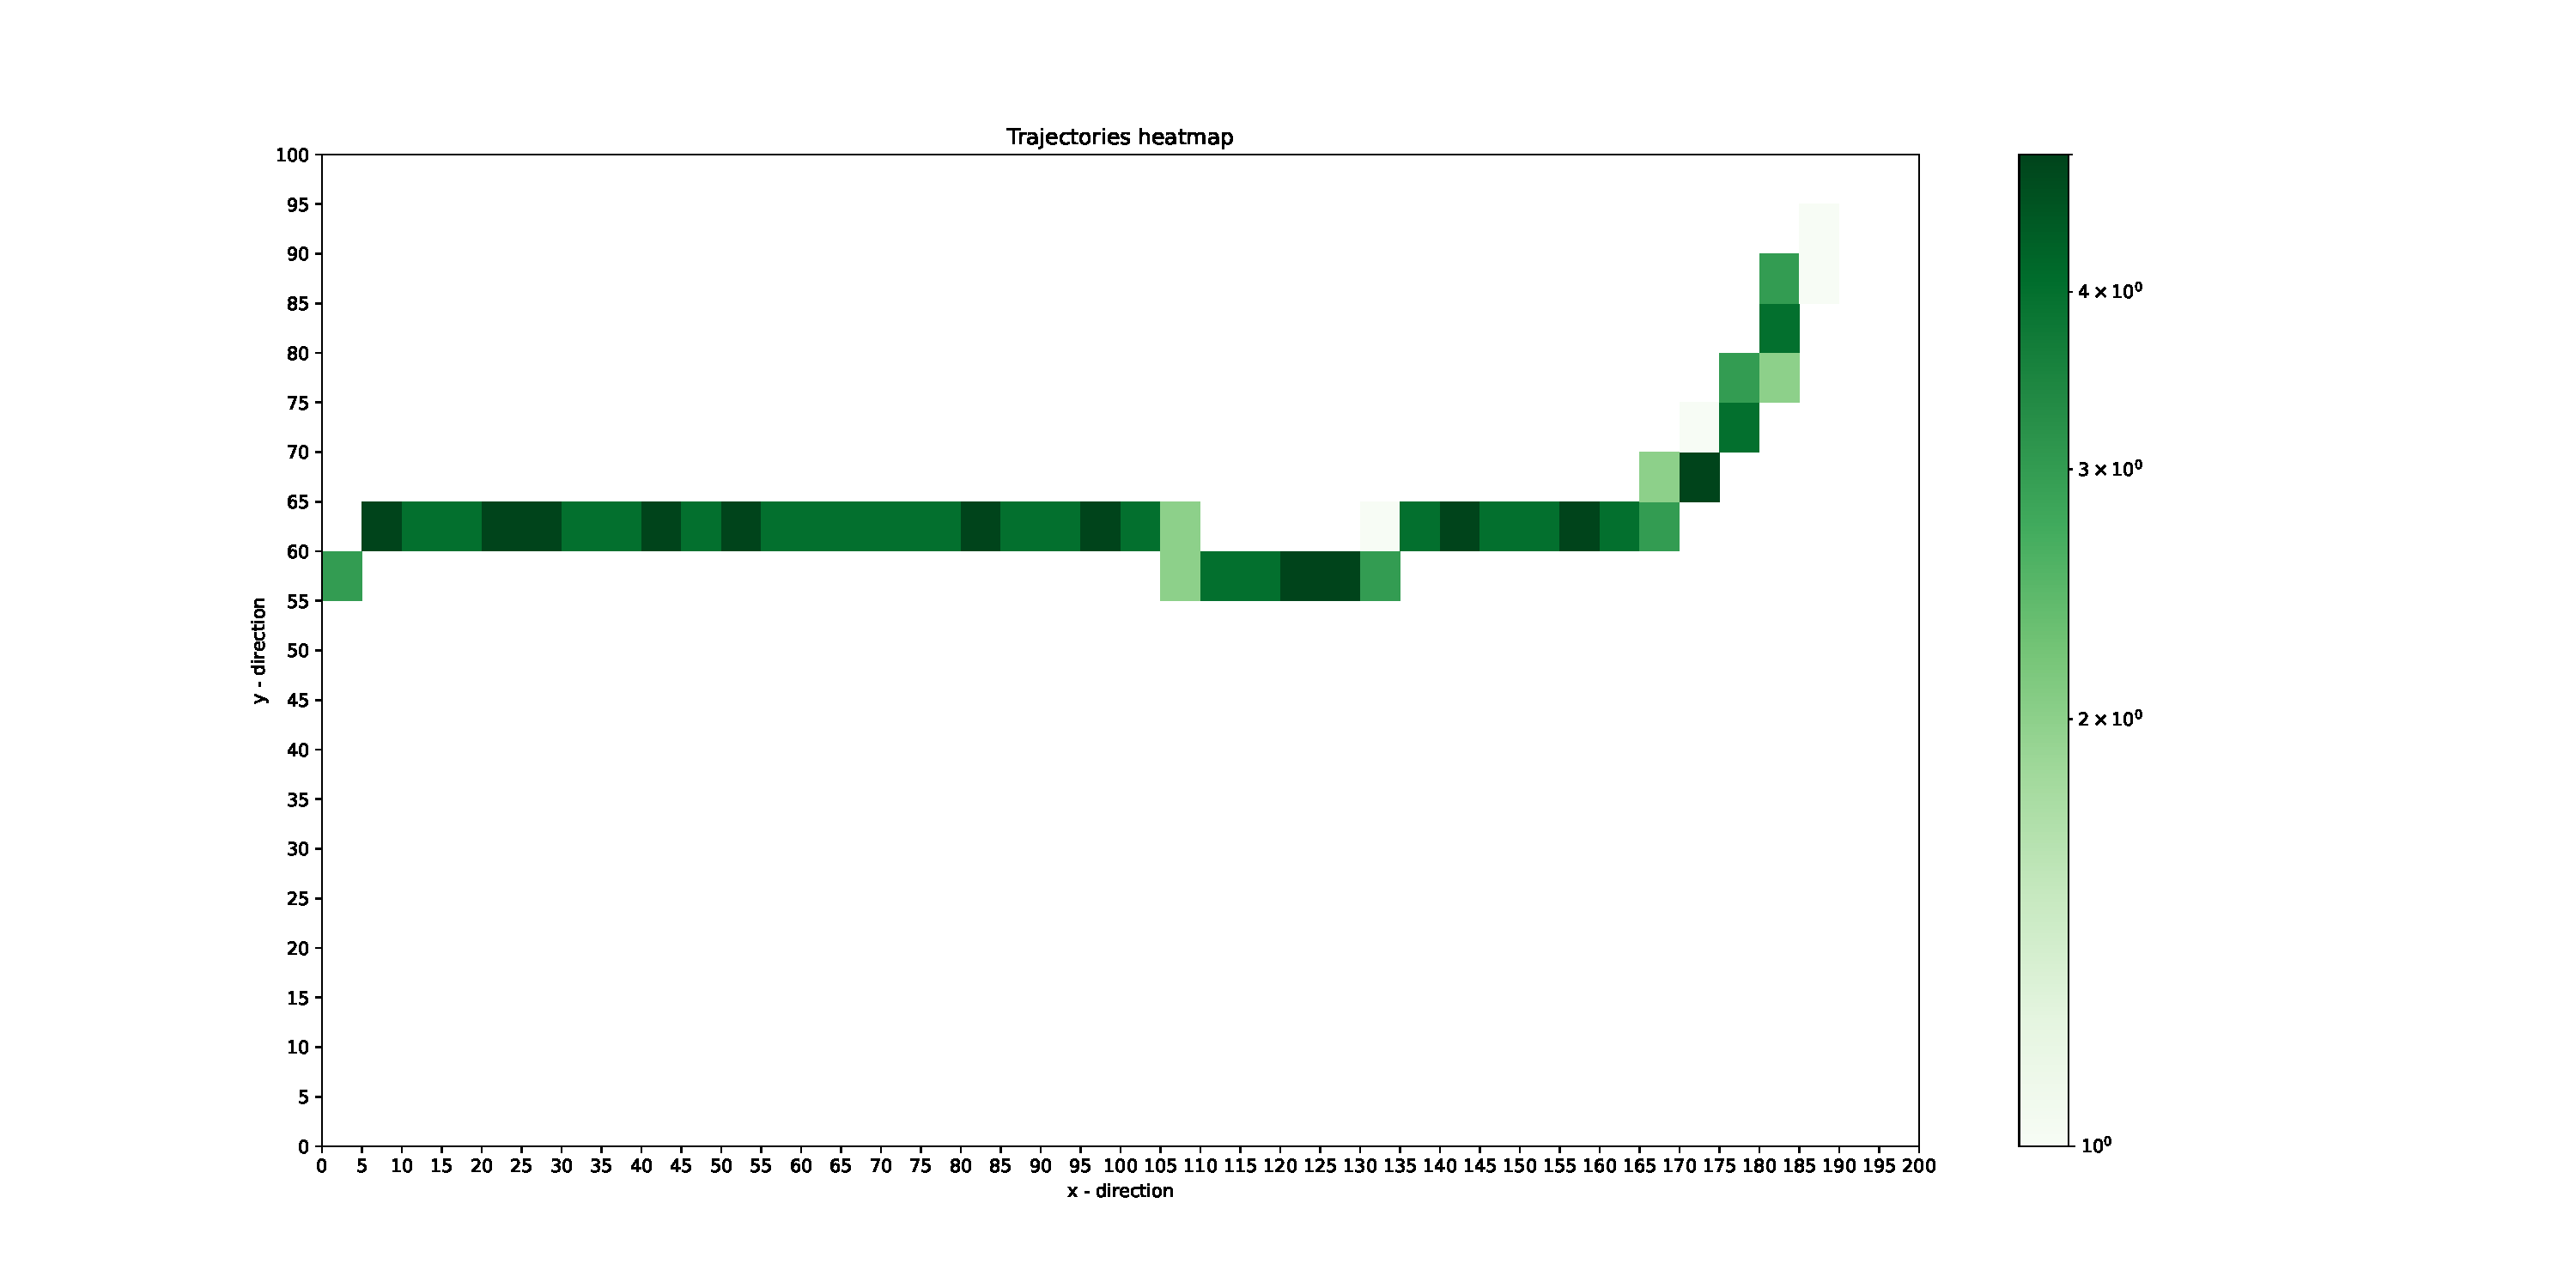
\includegraphics[ width=1\textwidth]{fig/belle_traiettorie/nice selection/figure_trainf10_RealData_heatmap_19marzo_select_single_NP_19_13140176}
\captionsetup{width=.8\linewidth}
\caption{Plot H, path 4}
\label{fig:semi_straight_up_H}
\end{minipage}
\begin{minipage}[c]{0.25\linewidth}
\centering
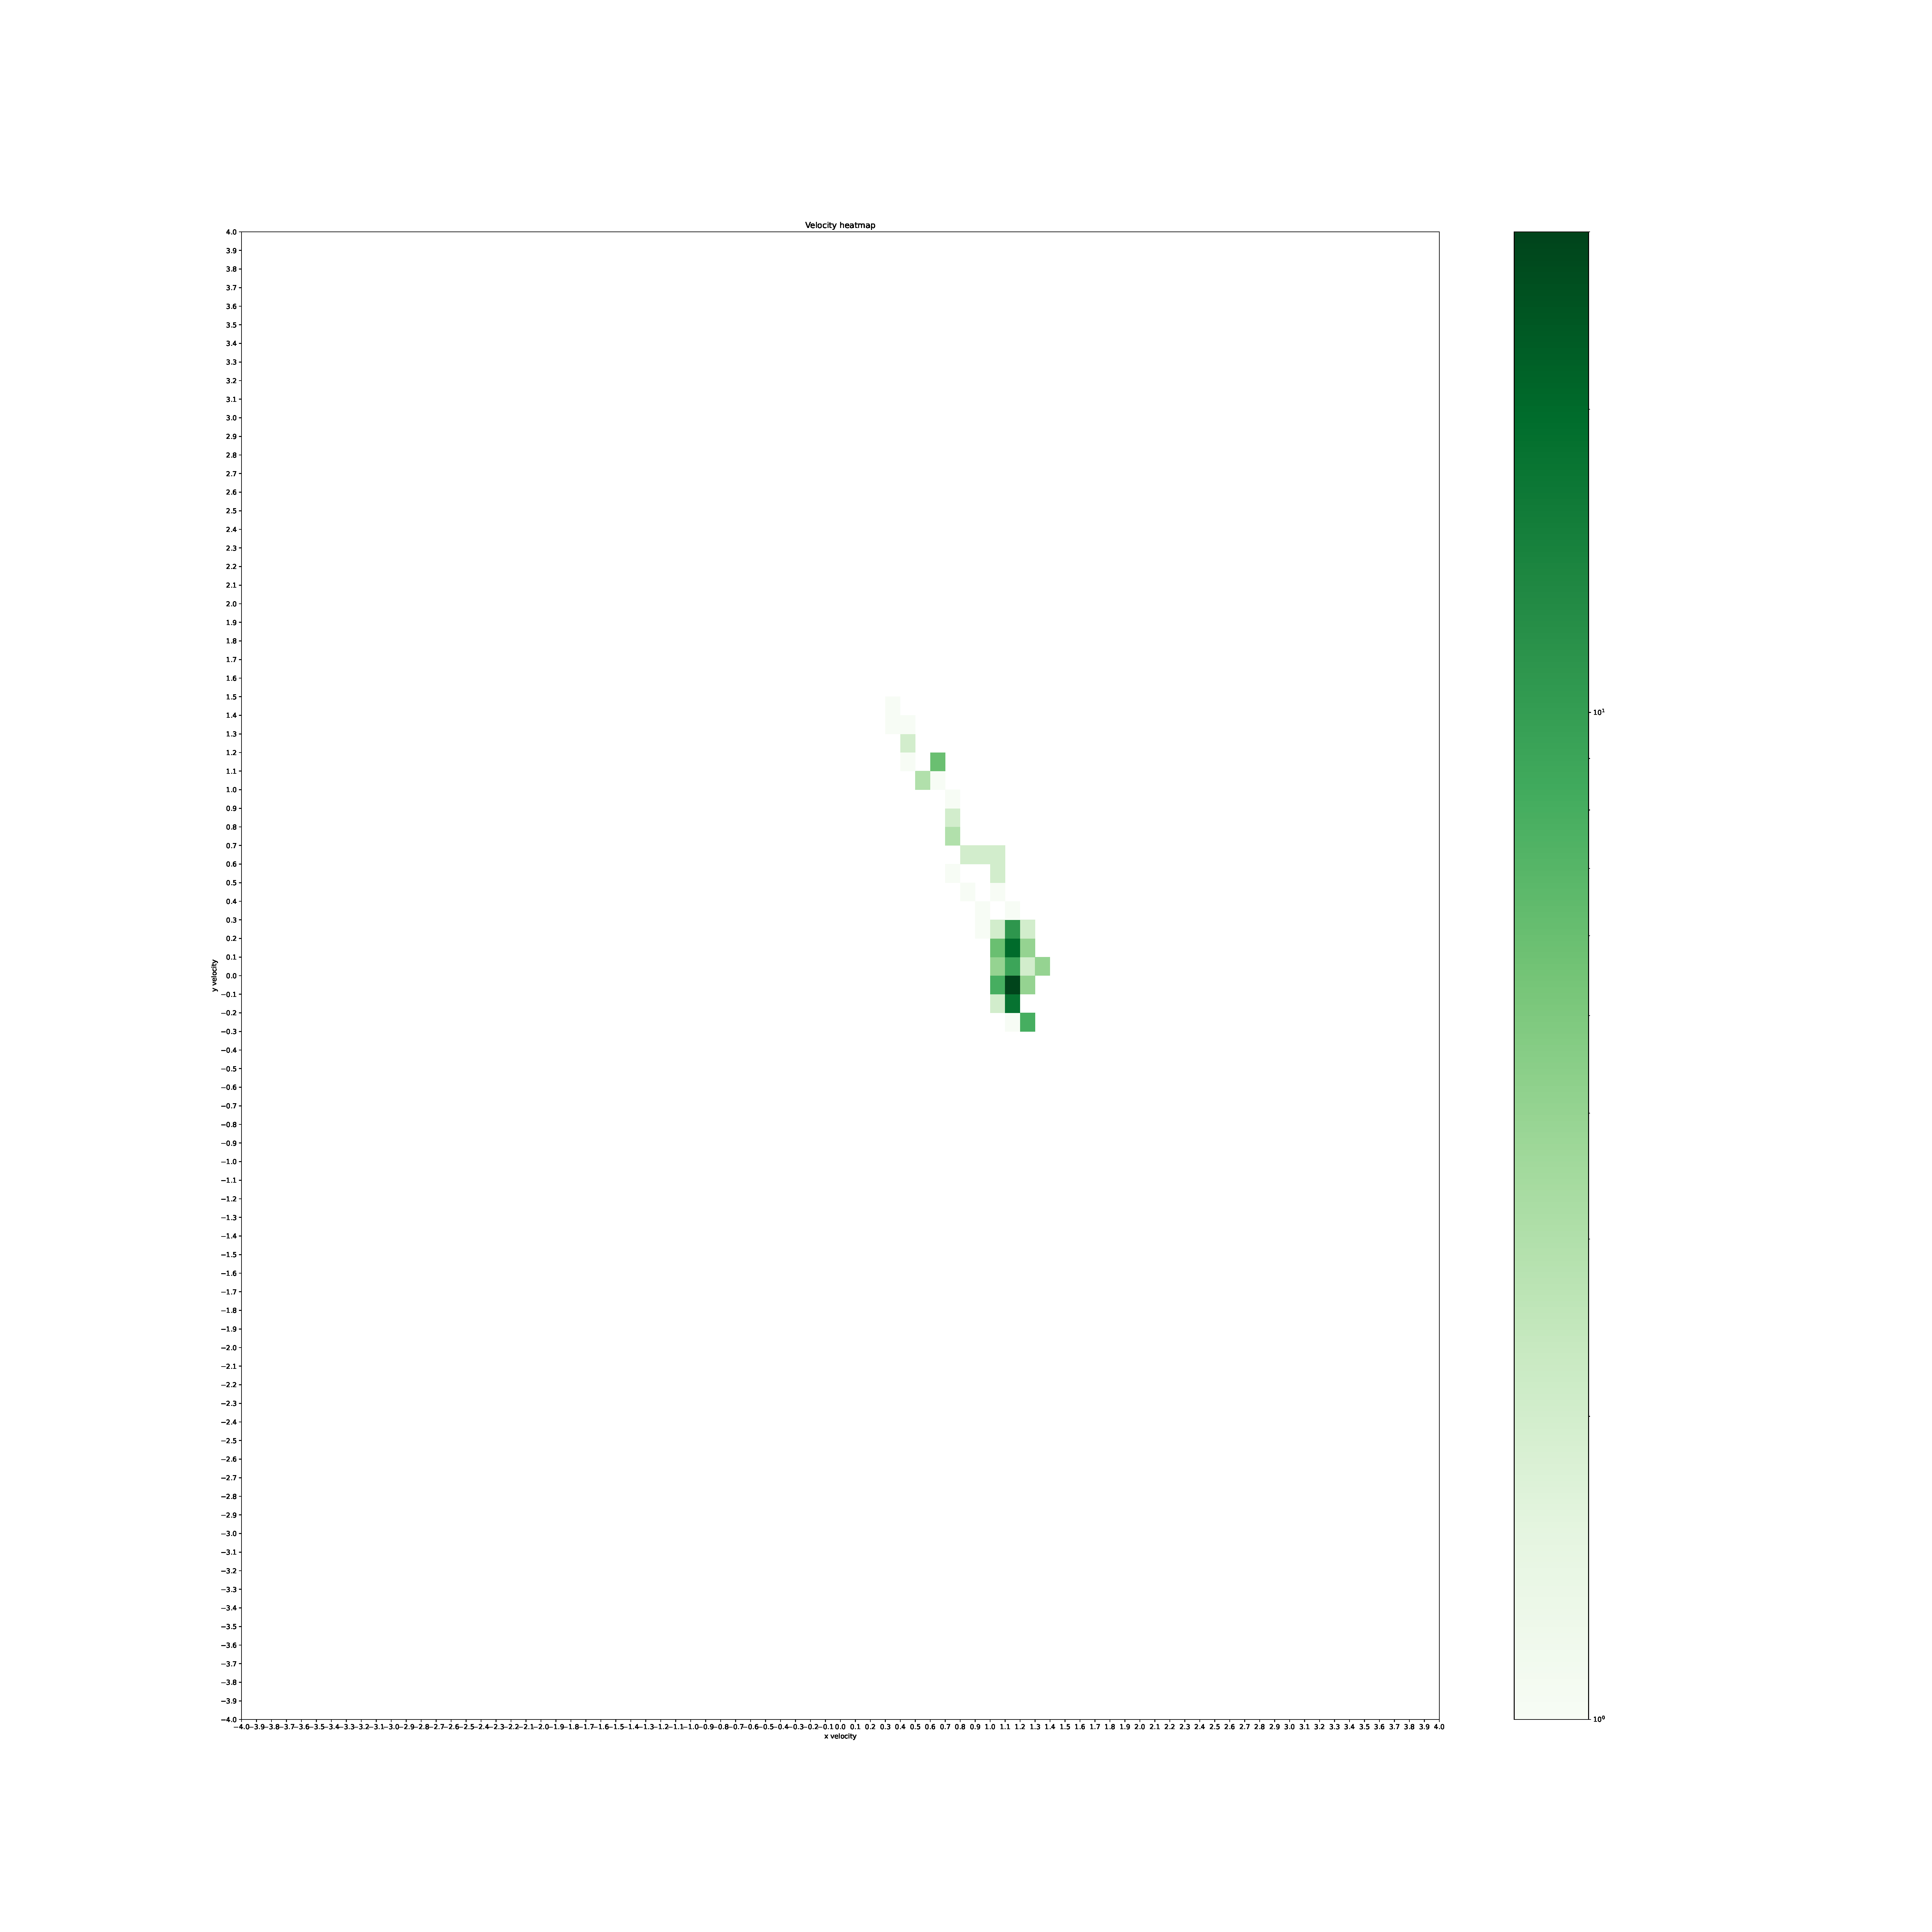
\includegraphics[ width=0.9\textwidth]{fig/belle_traiettorie/nice selection/figure_trainf10_RealData_velocity_heatmap_19marzo_select_single_NP_19_13140176}
\captionsetup{width=.8\linewidth}
\caption{Plot V, path 4}
\label{fig:semi_straight_up_V}
\end{minipage}
\end{figure}

% --- --- --- --- --- --- --- --- --- --- --- --- --- --- --- --- --- --- --- --- --- --- --- --- --- --- --- --- ---
\FloatBarrier
\newpage
Other paths are stranger than the previous.
Some trajectories are showed in (Figure \ref{fig:stranger_i} - \ref{fig:stranger_f}).
\\Then a few trajectories are presented together in (Figure \ref{fig:alltog_i} - \ref{fig:alltog_f}), 
to get the idea of how the entire dataset may became adding thousands of paths together.

\begin{figure}[ht]
\begin{minipage}[c]{0.35\linewidth}
\centering
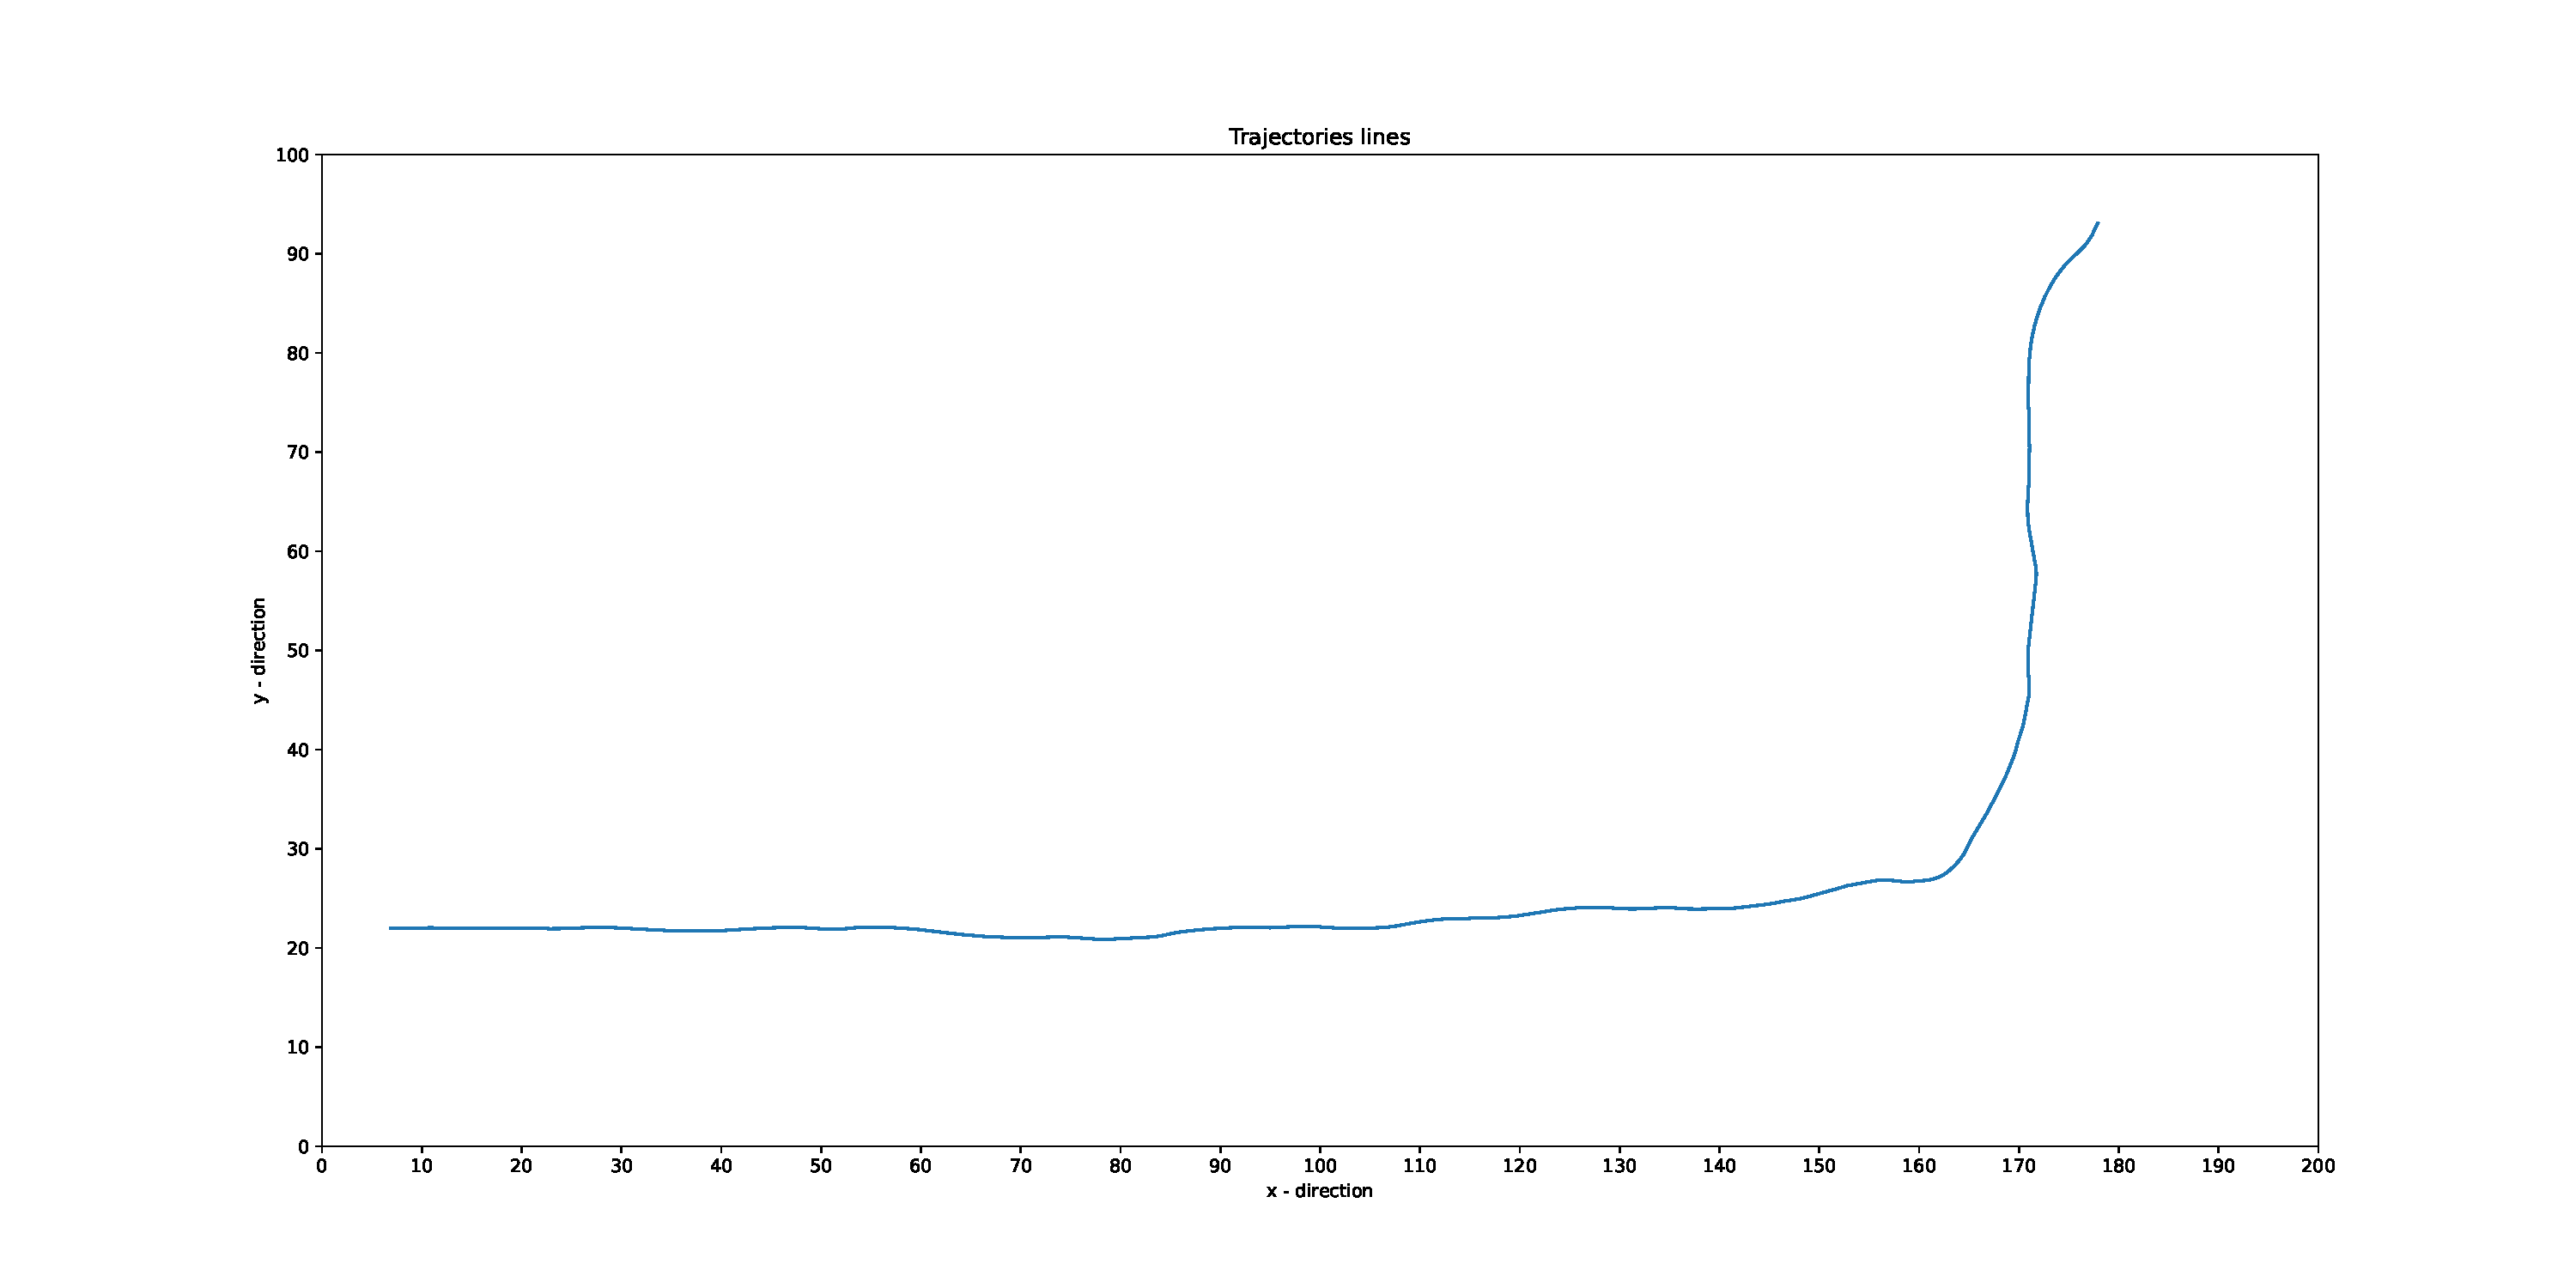
\includegraphics[ width=1\textwidth]{fig/belle_traiettorie/nice selection/figure_trainf10_RealData_lines_19marzo_select_single_NP_19_13075004}
\captionsetup{width=.8\linewidth}
\caption{Plot L}
\label{fig:stranger_i}
\end{minipage}
\begin{minipage}[c]{0.35\linewidth}
\centering
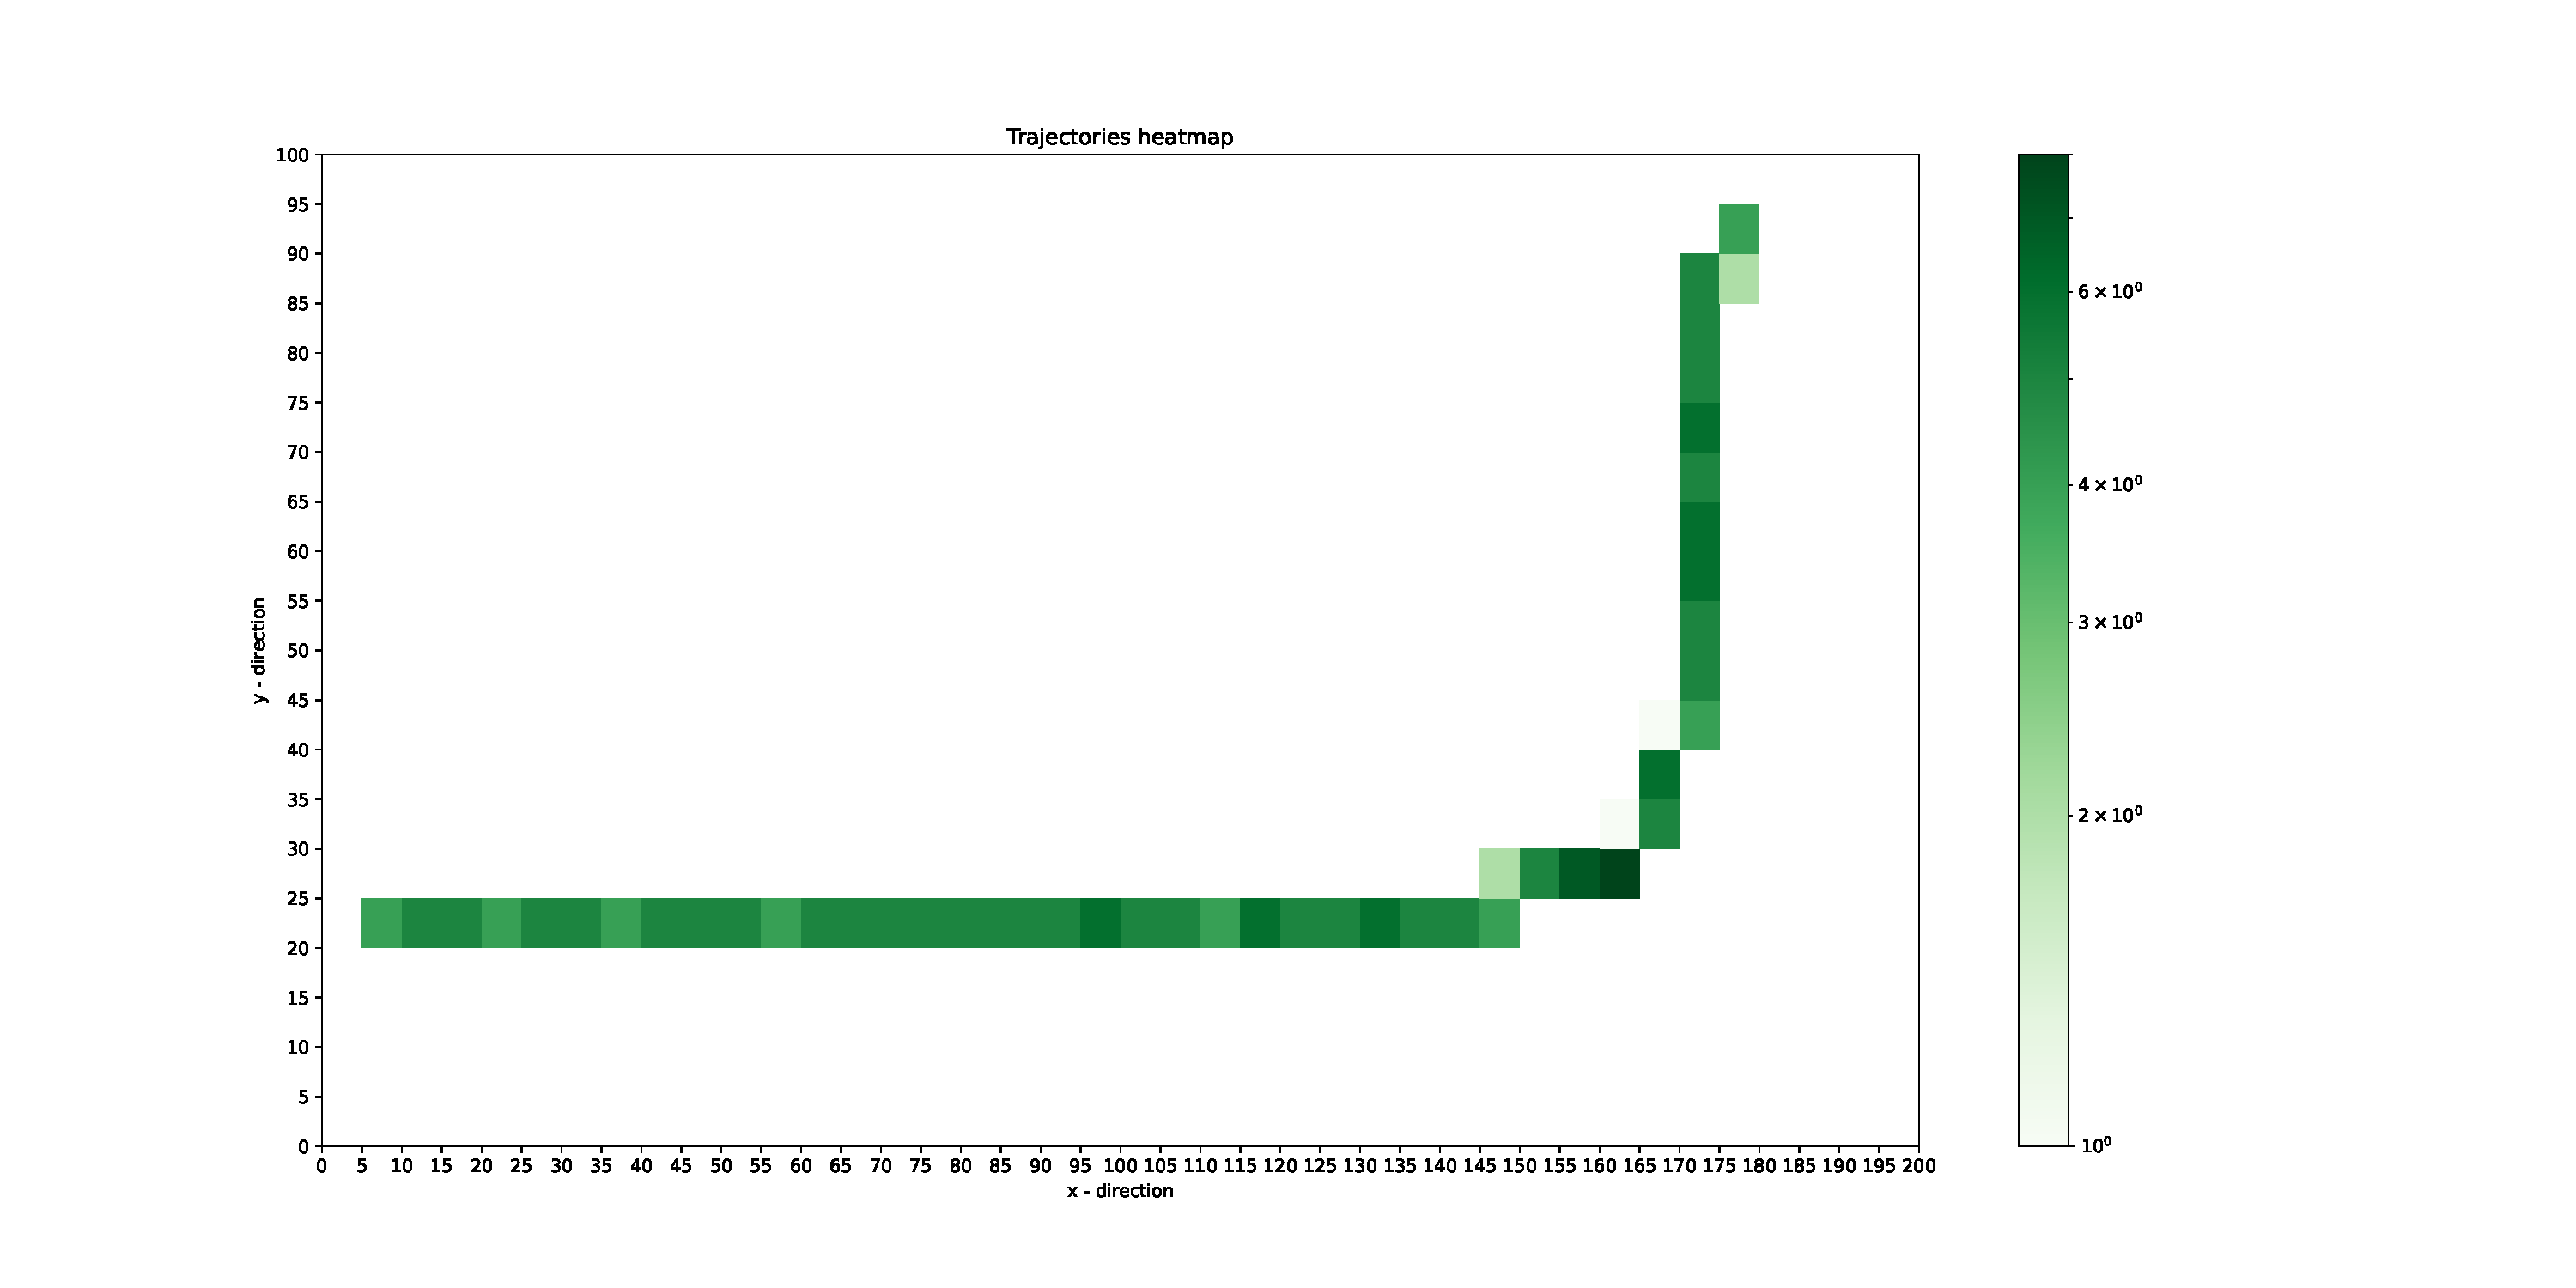
\includegraphics[ width=1\textwidth]{fig/belle_traiettorie/nice selection/figure_trainf10_RealData_heatmap_19marzo_select_single_NP_19_13075004}
\captionsetup{width=.8\linewidth}
\caption{Plot H}
%\label{fig:stranger_i}
\end{minipage}
\begin{minipage}[c]{0.25\linewidth}
\centering
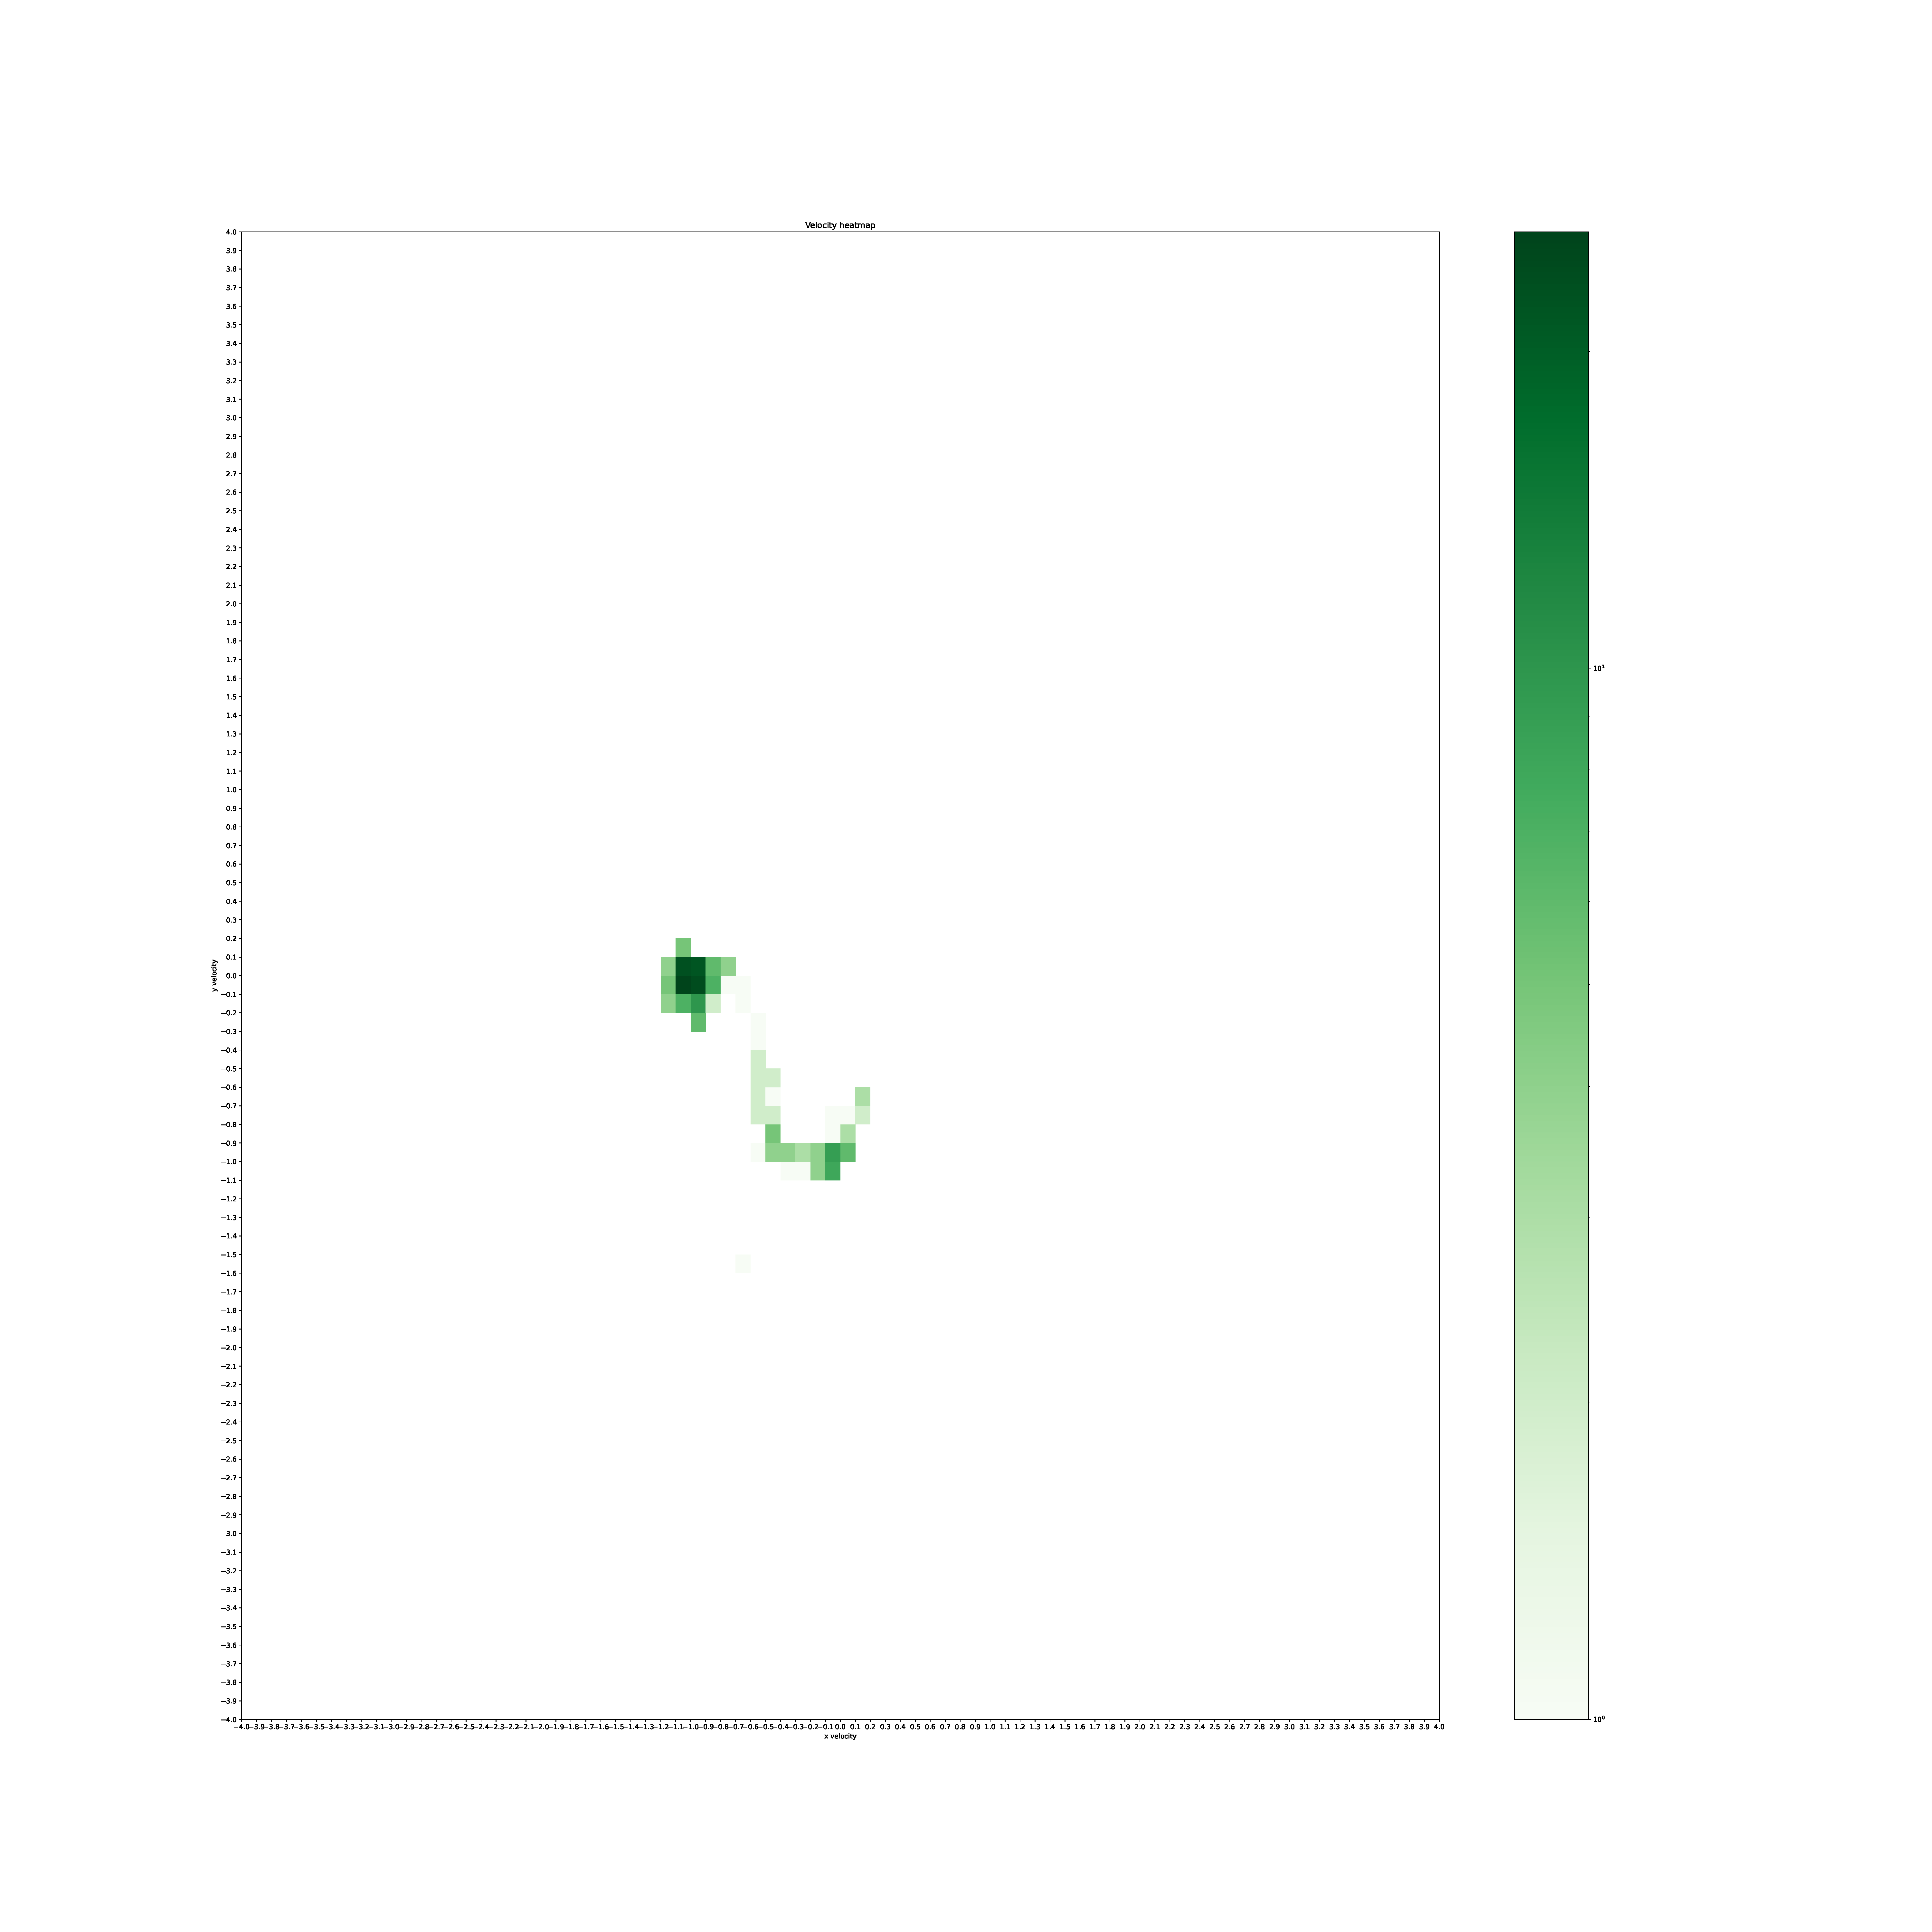
\includegraphics[ width=0.9\textwidth]{fig/belle_traiettorie/nice selection/figure_trainf10_RealData_velocity_heatmap_19marzo_select_single_NP_19_13075004}
\captionsetup{width=.8\linewidth}
\caption{Plot V}
%\label{fig:stranger_f}
\end{minipage}
% --- --- --- --- --- --- --- --- --- --- --- --- --- --- --- --- --- --- --- --- --- --- --- --- --- --- --- --- ---
\vspace*{5mm}
\begin{minipage}[c]{0.35\linewidth}
\centering
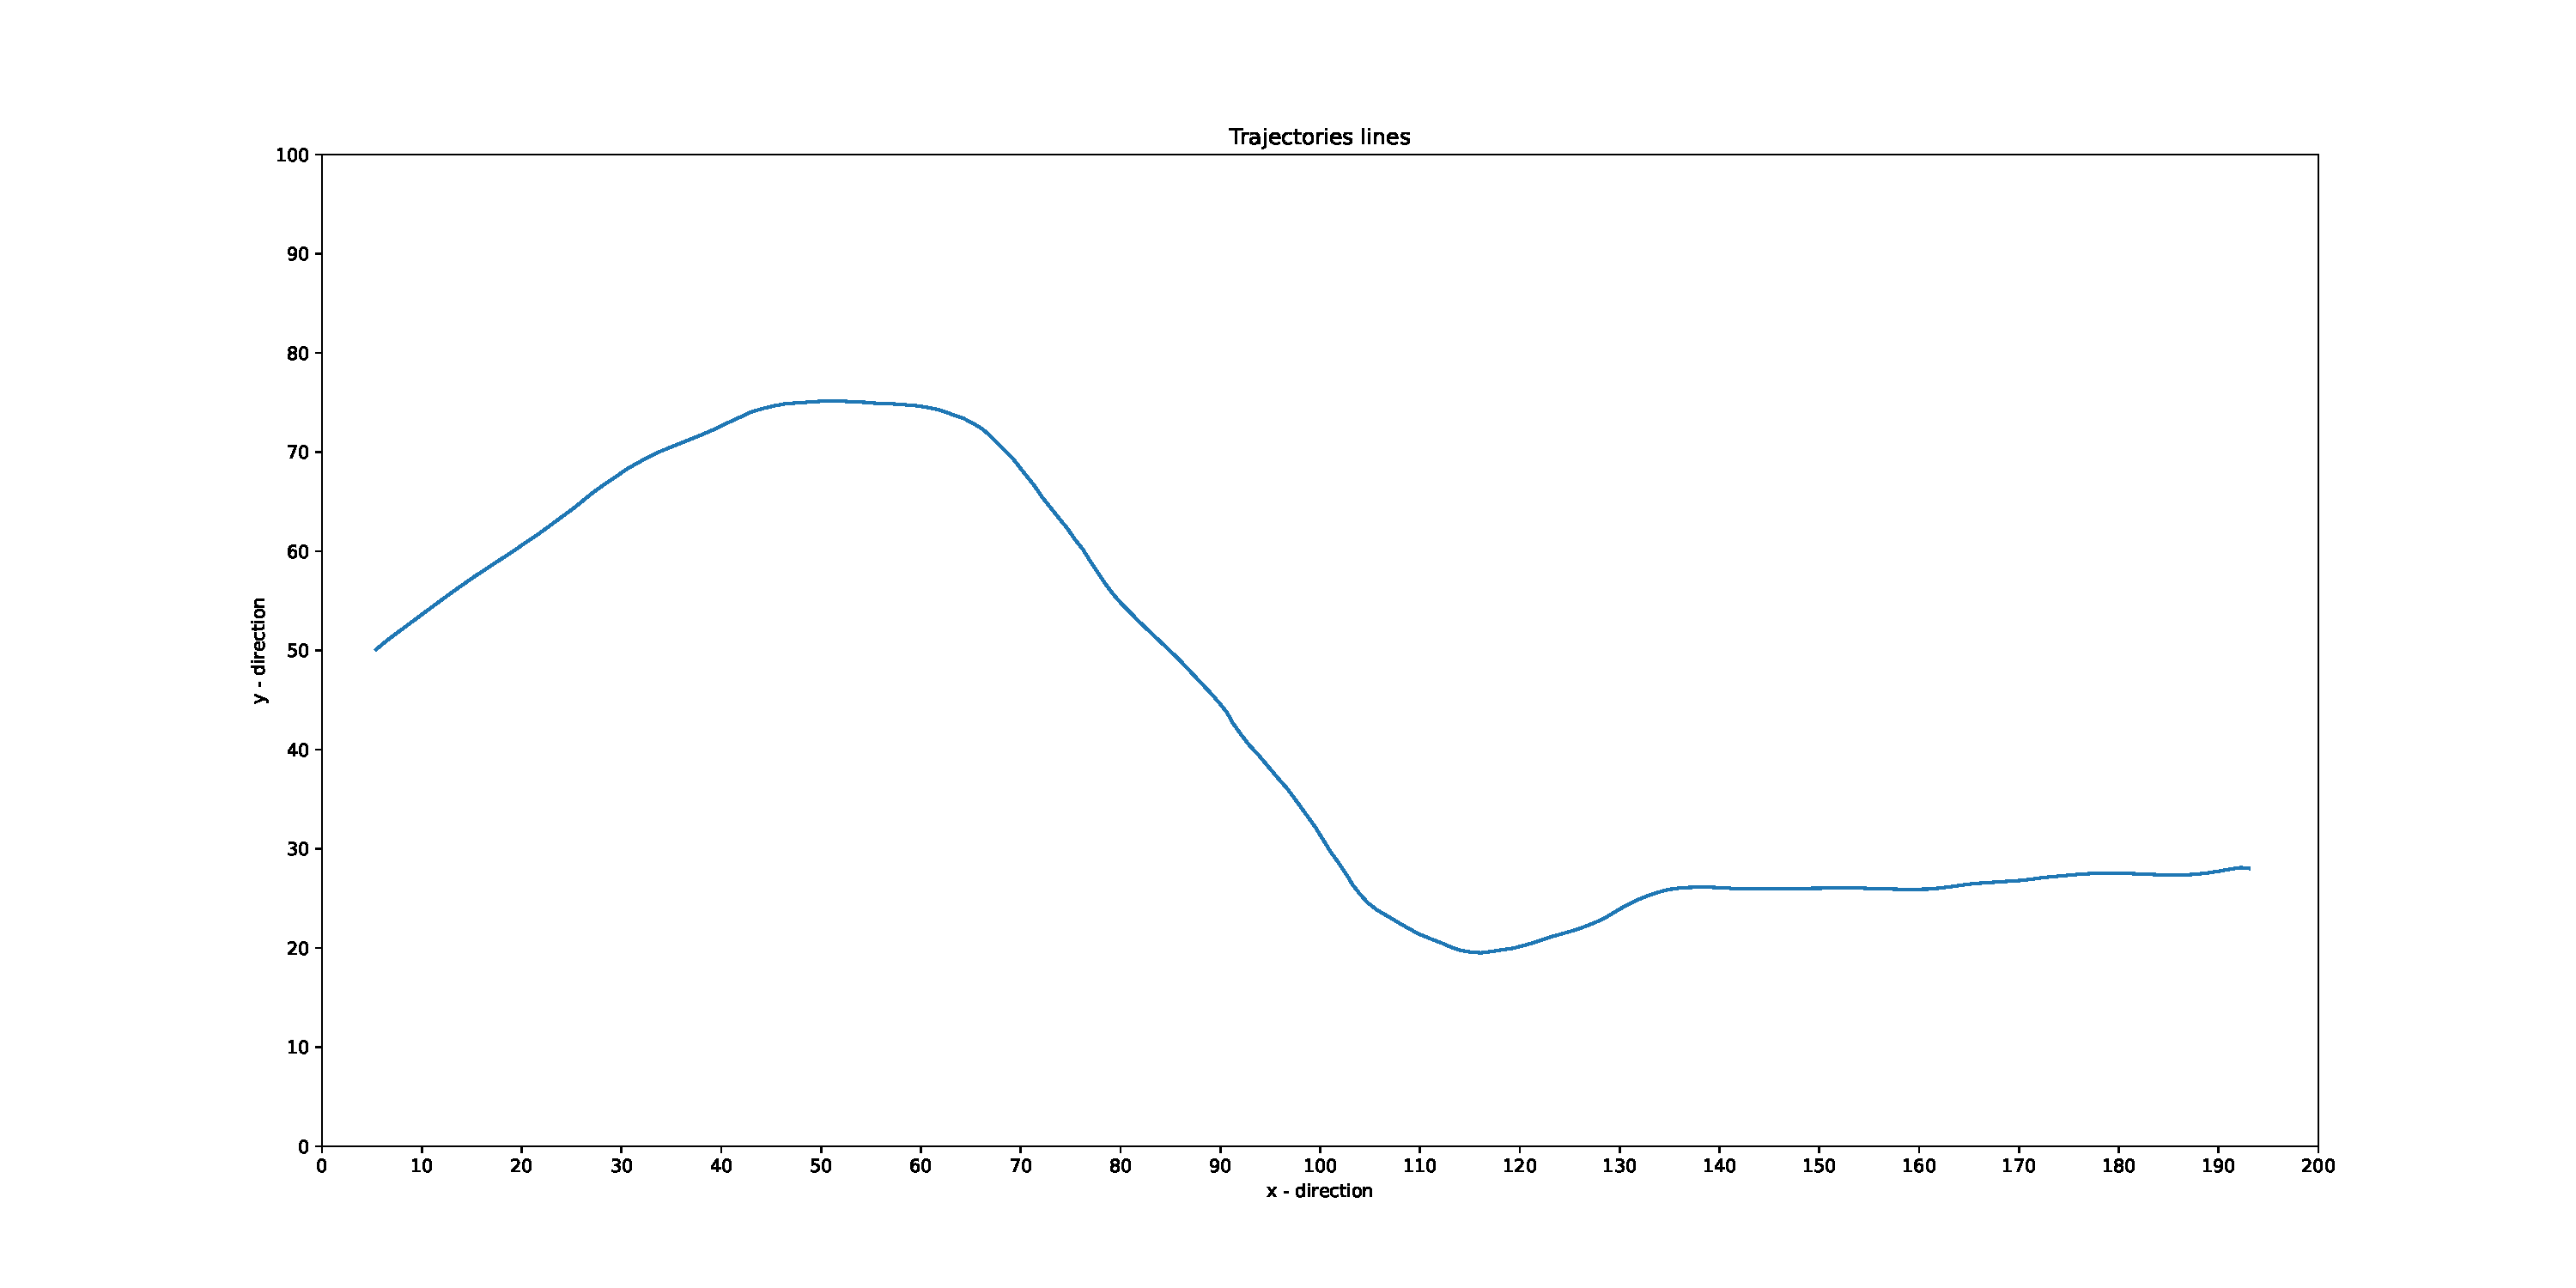
\includegraphics[ width=1\textwidth]{fig/belle_traiettorie/nice selection/figure_trainf10_RealData_lines_19marzo_select_single_NP_19_13108050}
\captionsetup{width=.8\linewidth}
\caption{Plot L}
%\label{fig:stranger_i}
\end{minipage}
\begin{minipage}[c]{0.35\linewidth}
\centering
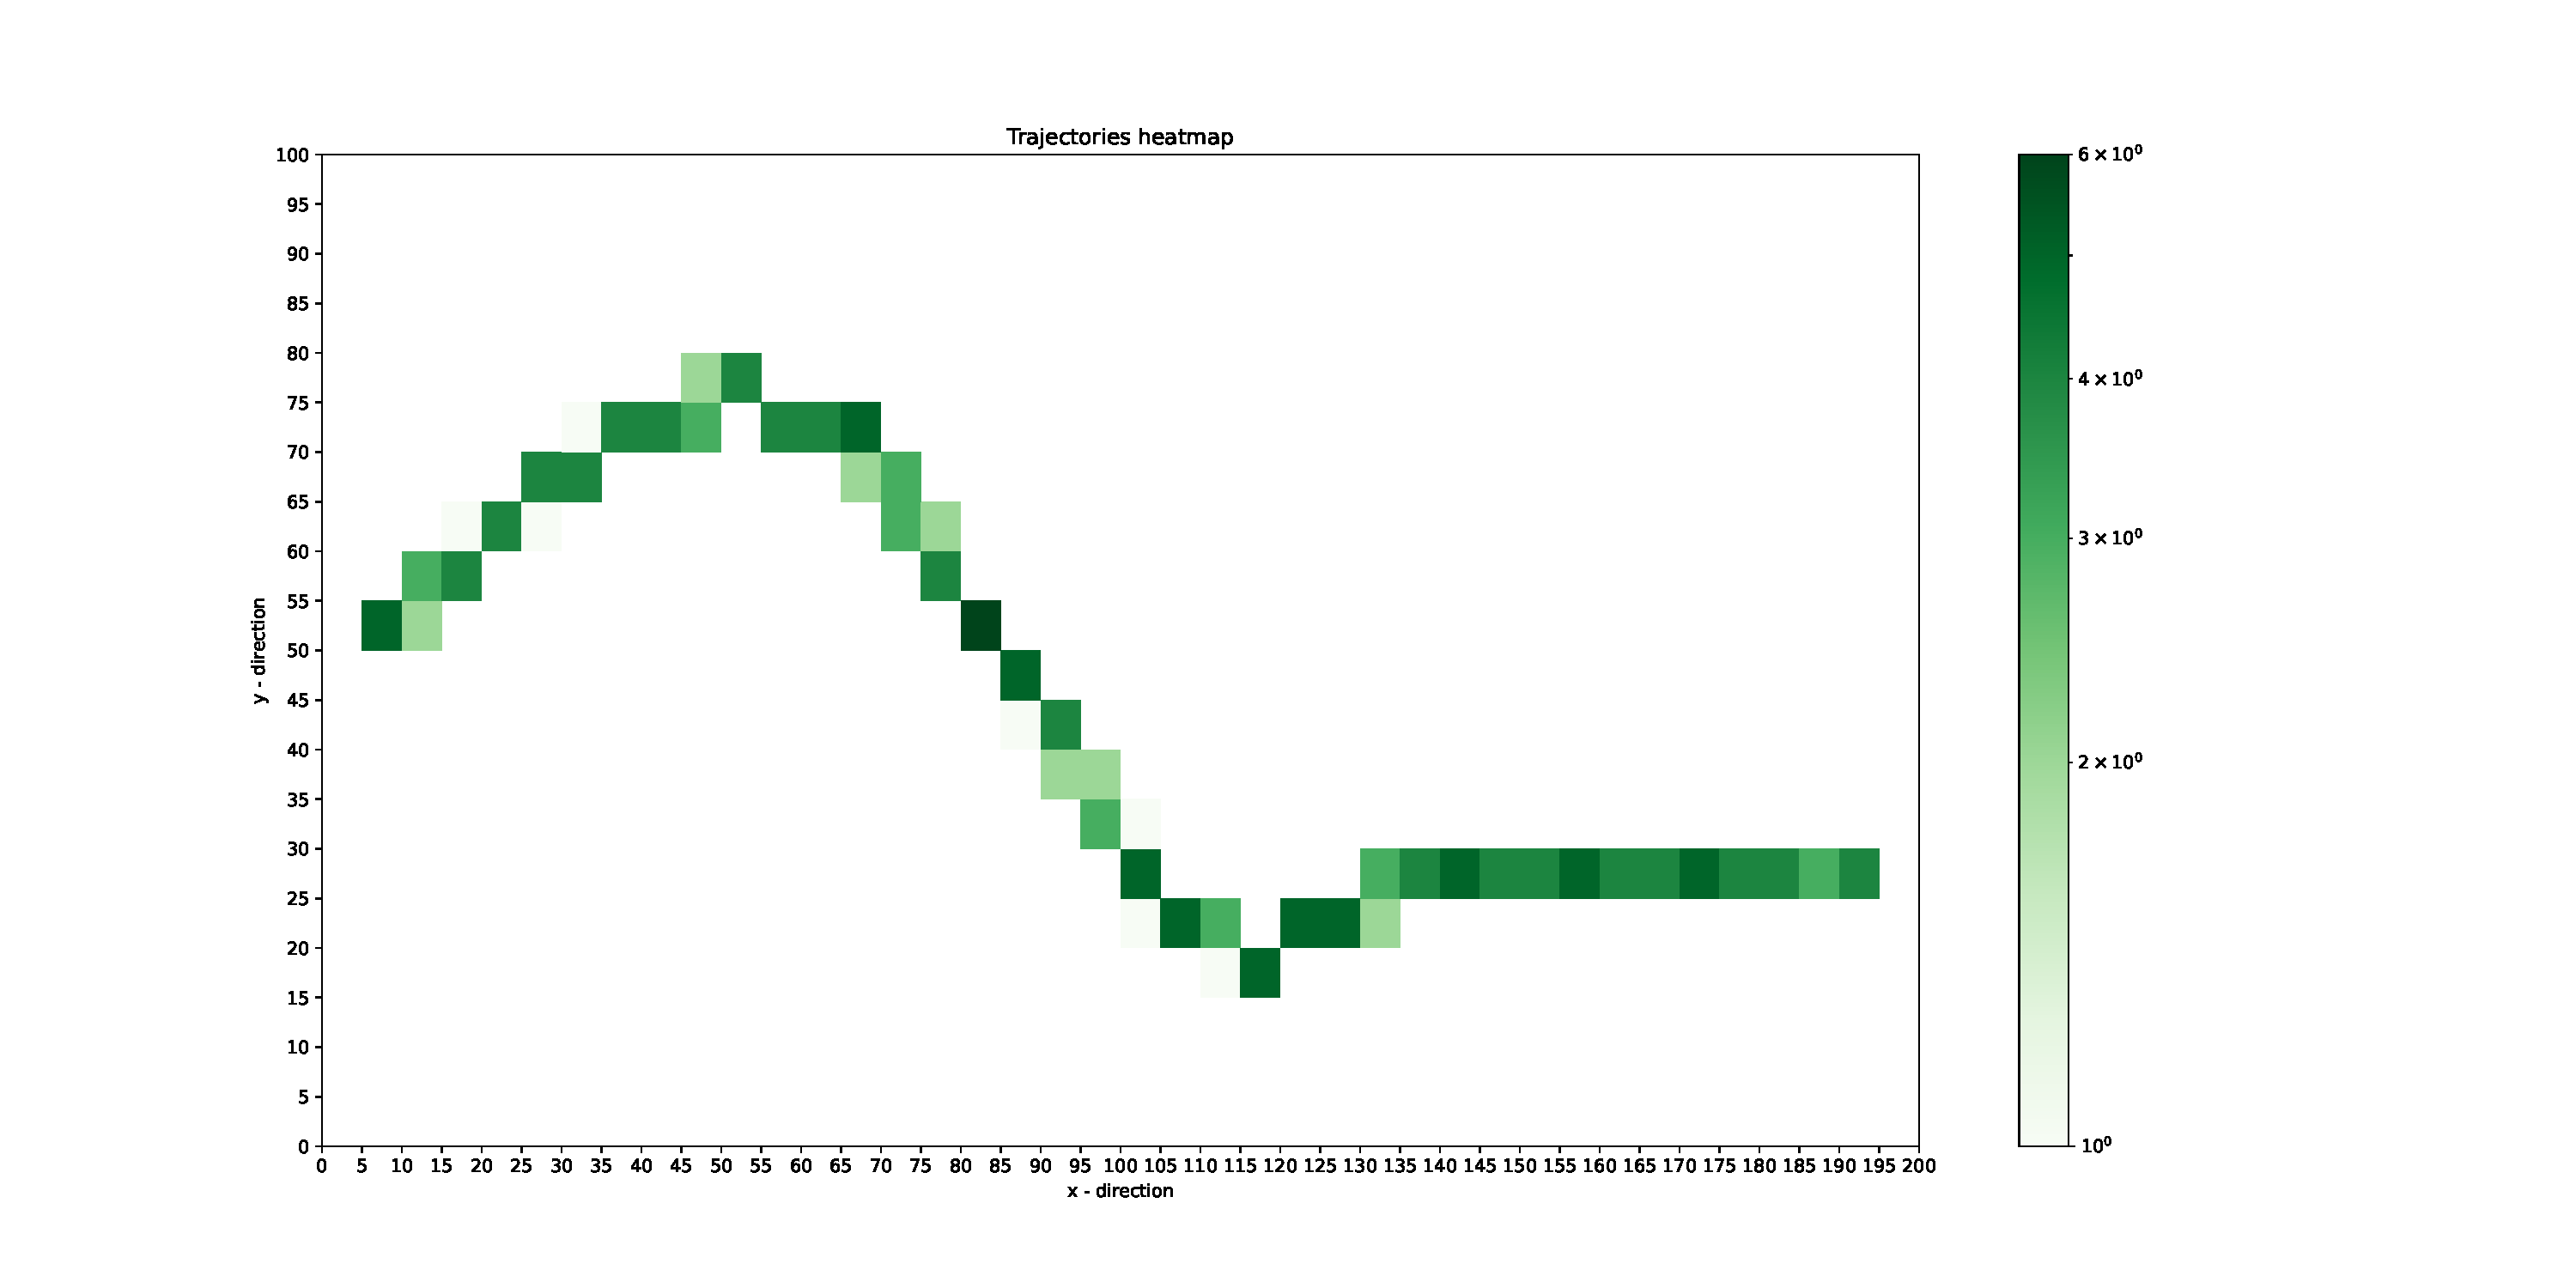
\includegraphics[ width=1\textwidth]{fig/belle_traiettorie/nice selection/figure_trainf10_RealData_heatmap_19marzo_select_single_NP_19_13108050}
\captionsetup{width=.8\linewidth}
\caption{Plot H}
%\label{fig:stranger_i}
\end{minipage}
\begin{minipage}[c]{0.25\linewidth}
\centering
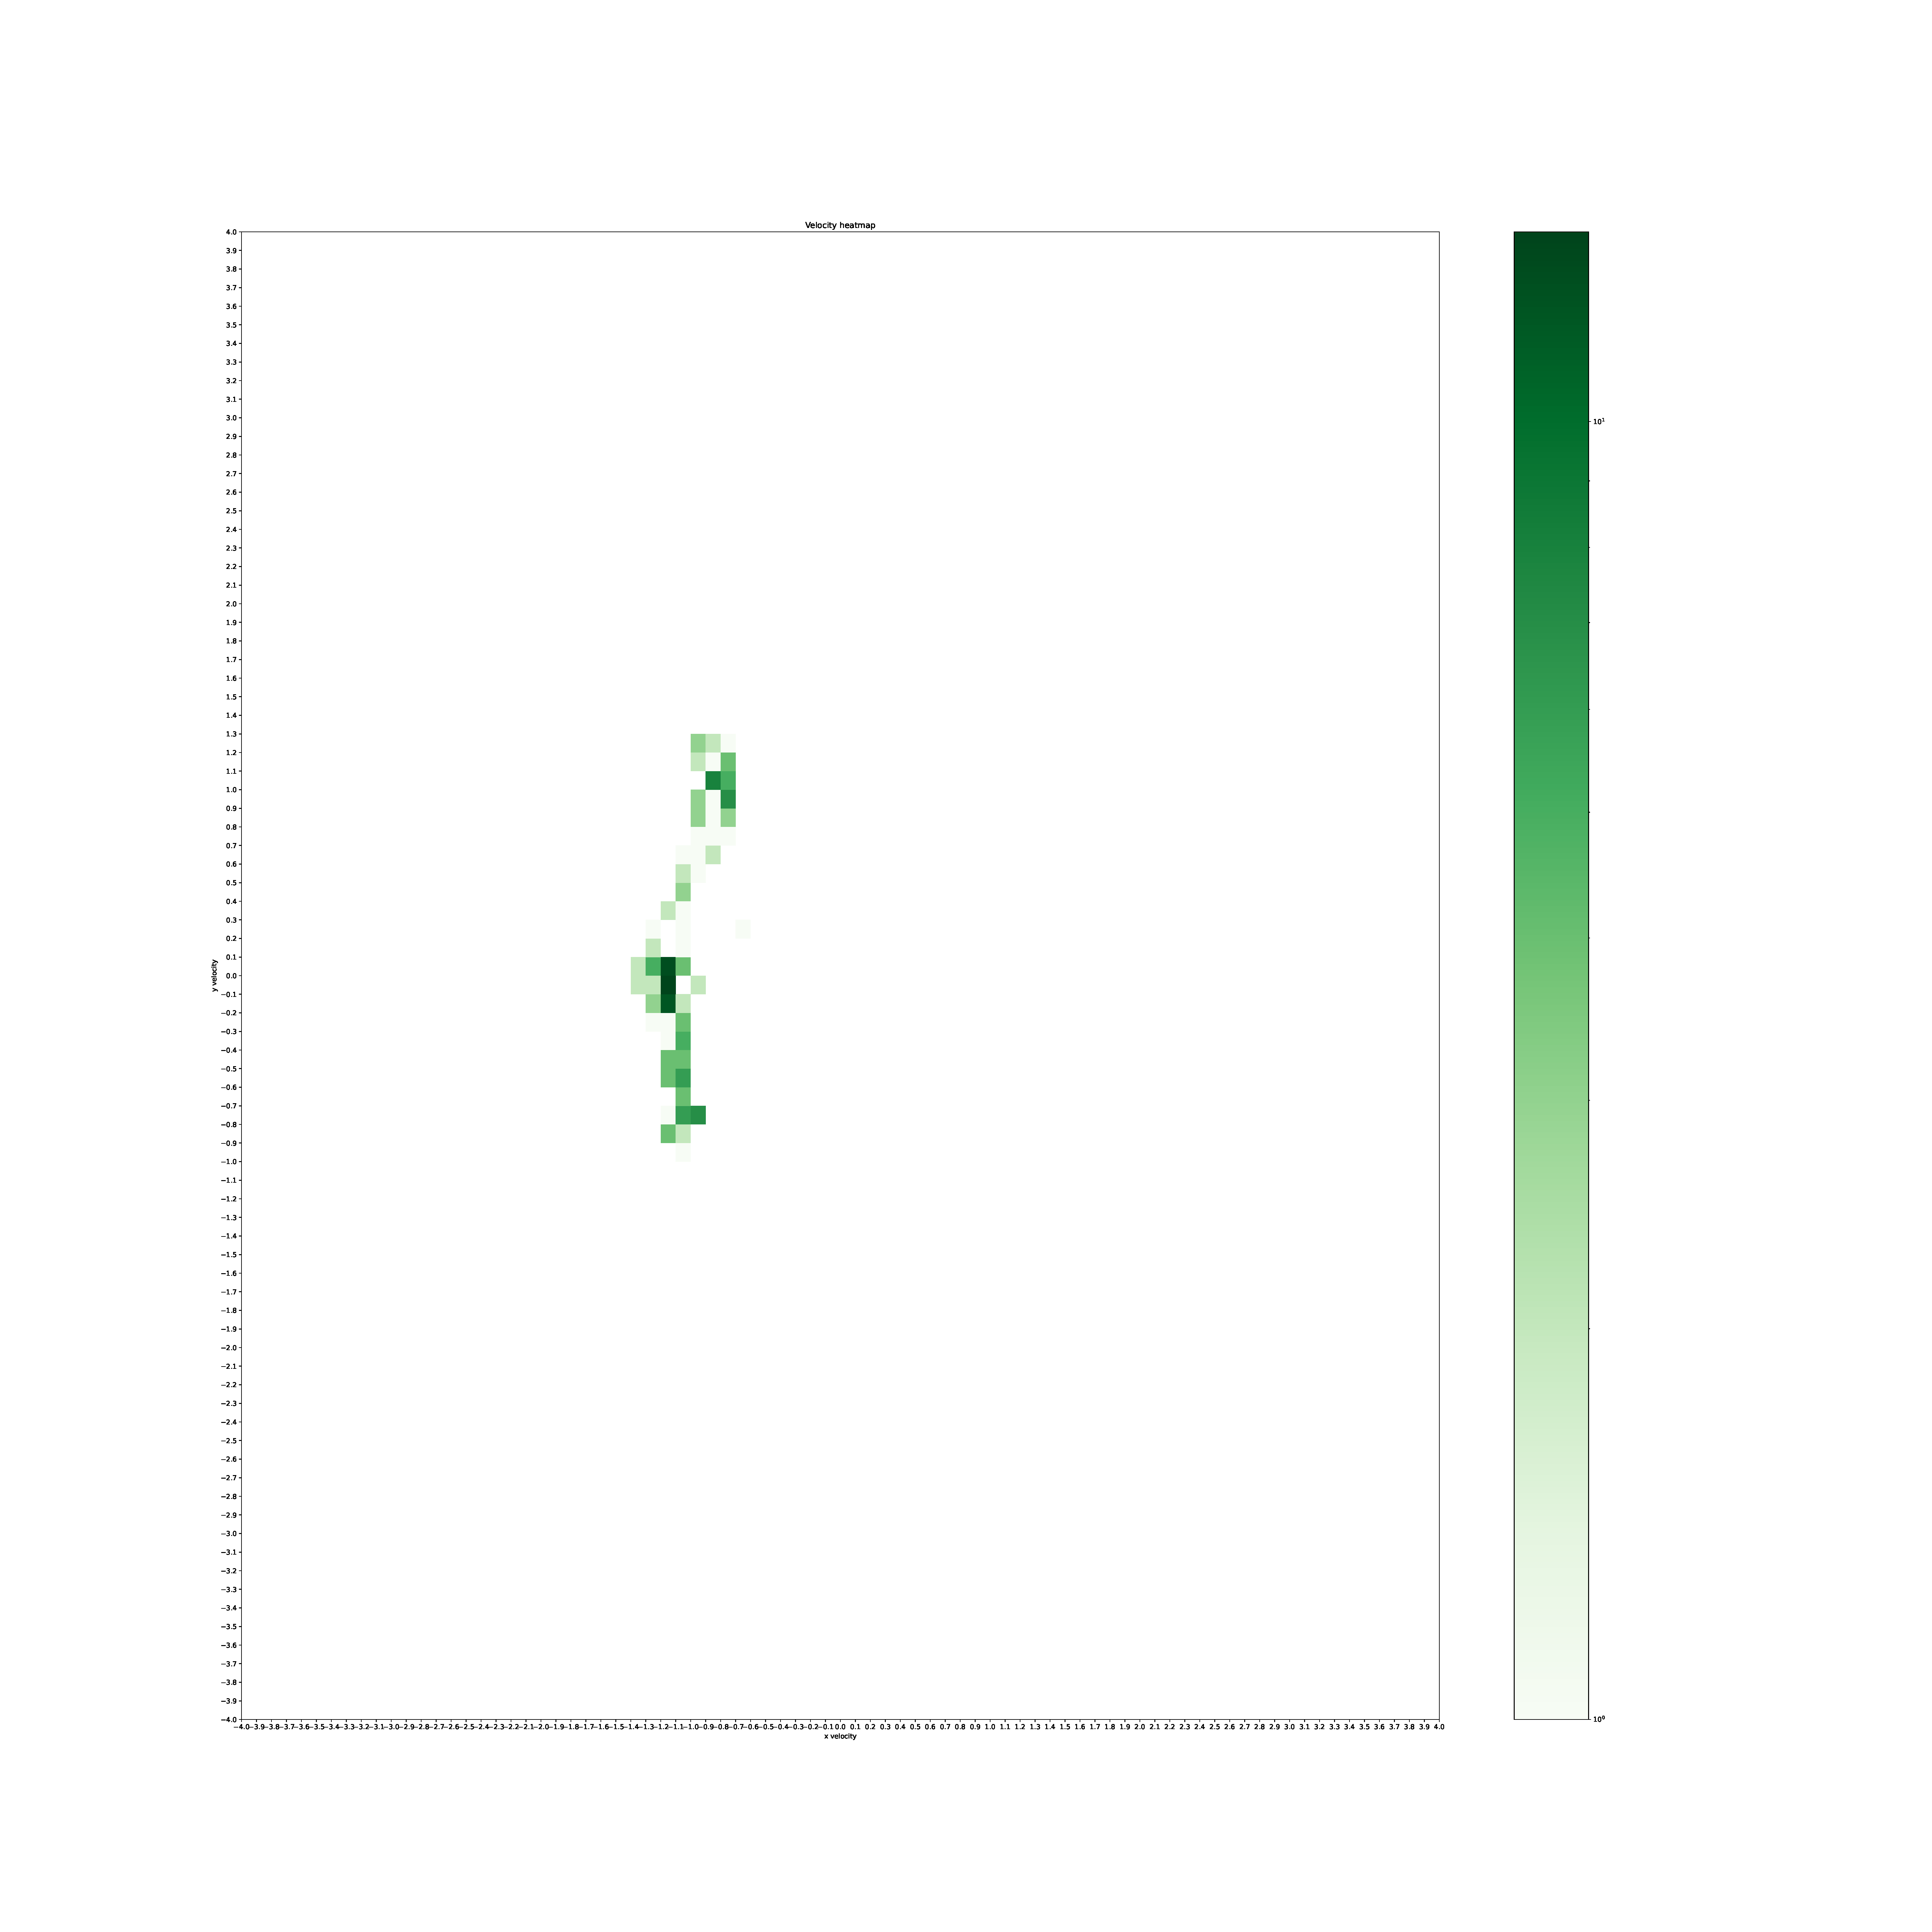
\includegraphics[ width=0.9\textwidth]{fig/belle_traiettorie/nice selection/figure_trainf10_RealData_velocity_heatmap_19marzo_select_single_NP_19_13108050}
\captionsetup{width=.8\linewidth}
\caption{Plot V}
%\label{fig:stranger_f}
\end{minipage}
% --- --- --- --- --- --- --- --- --- --- --- --- --- --- --- --- --- --- --- --- --- --- --- --- --- --- --- --- ---
\vspace*{5mm}
\begin{minipage}[c]{0.35\linewidth}
\centering
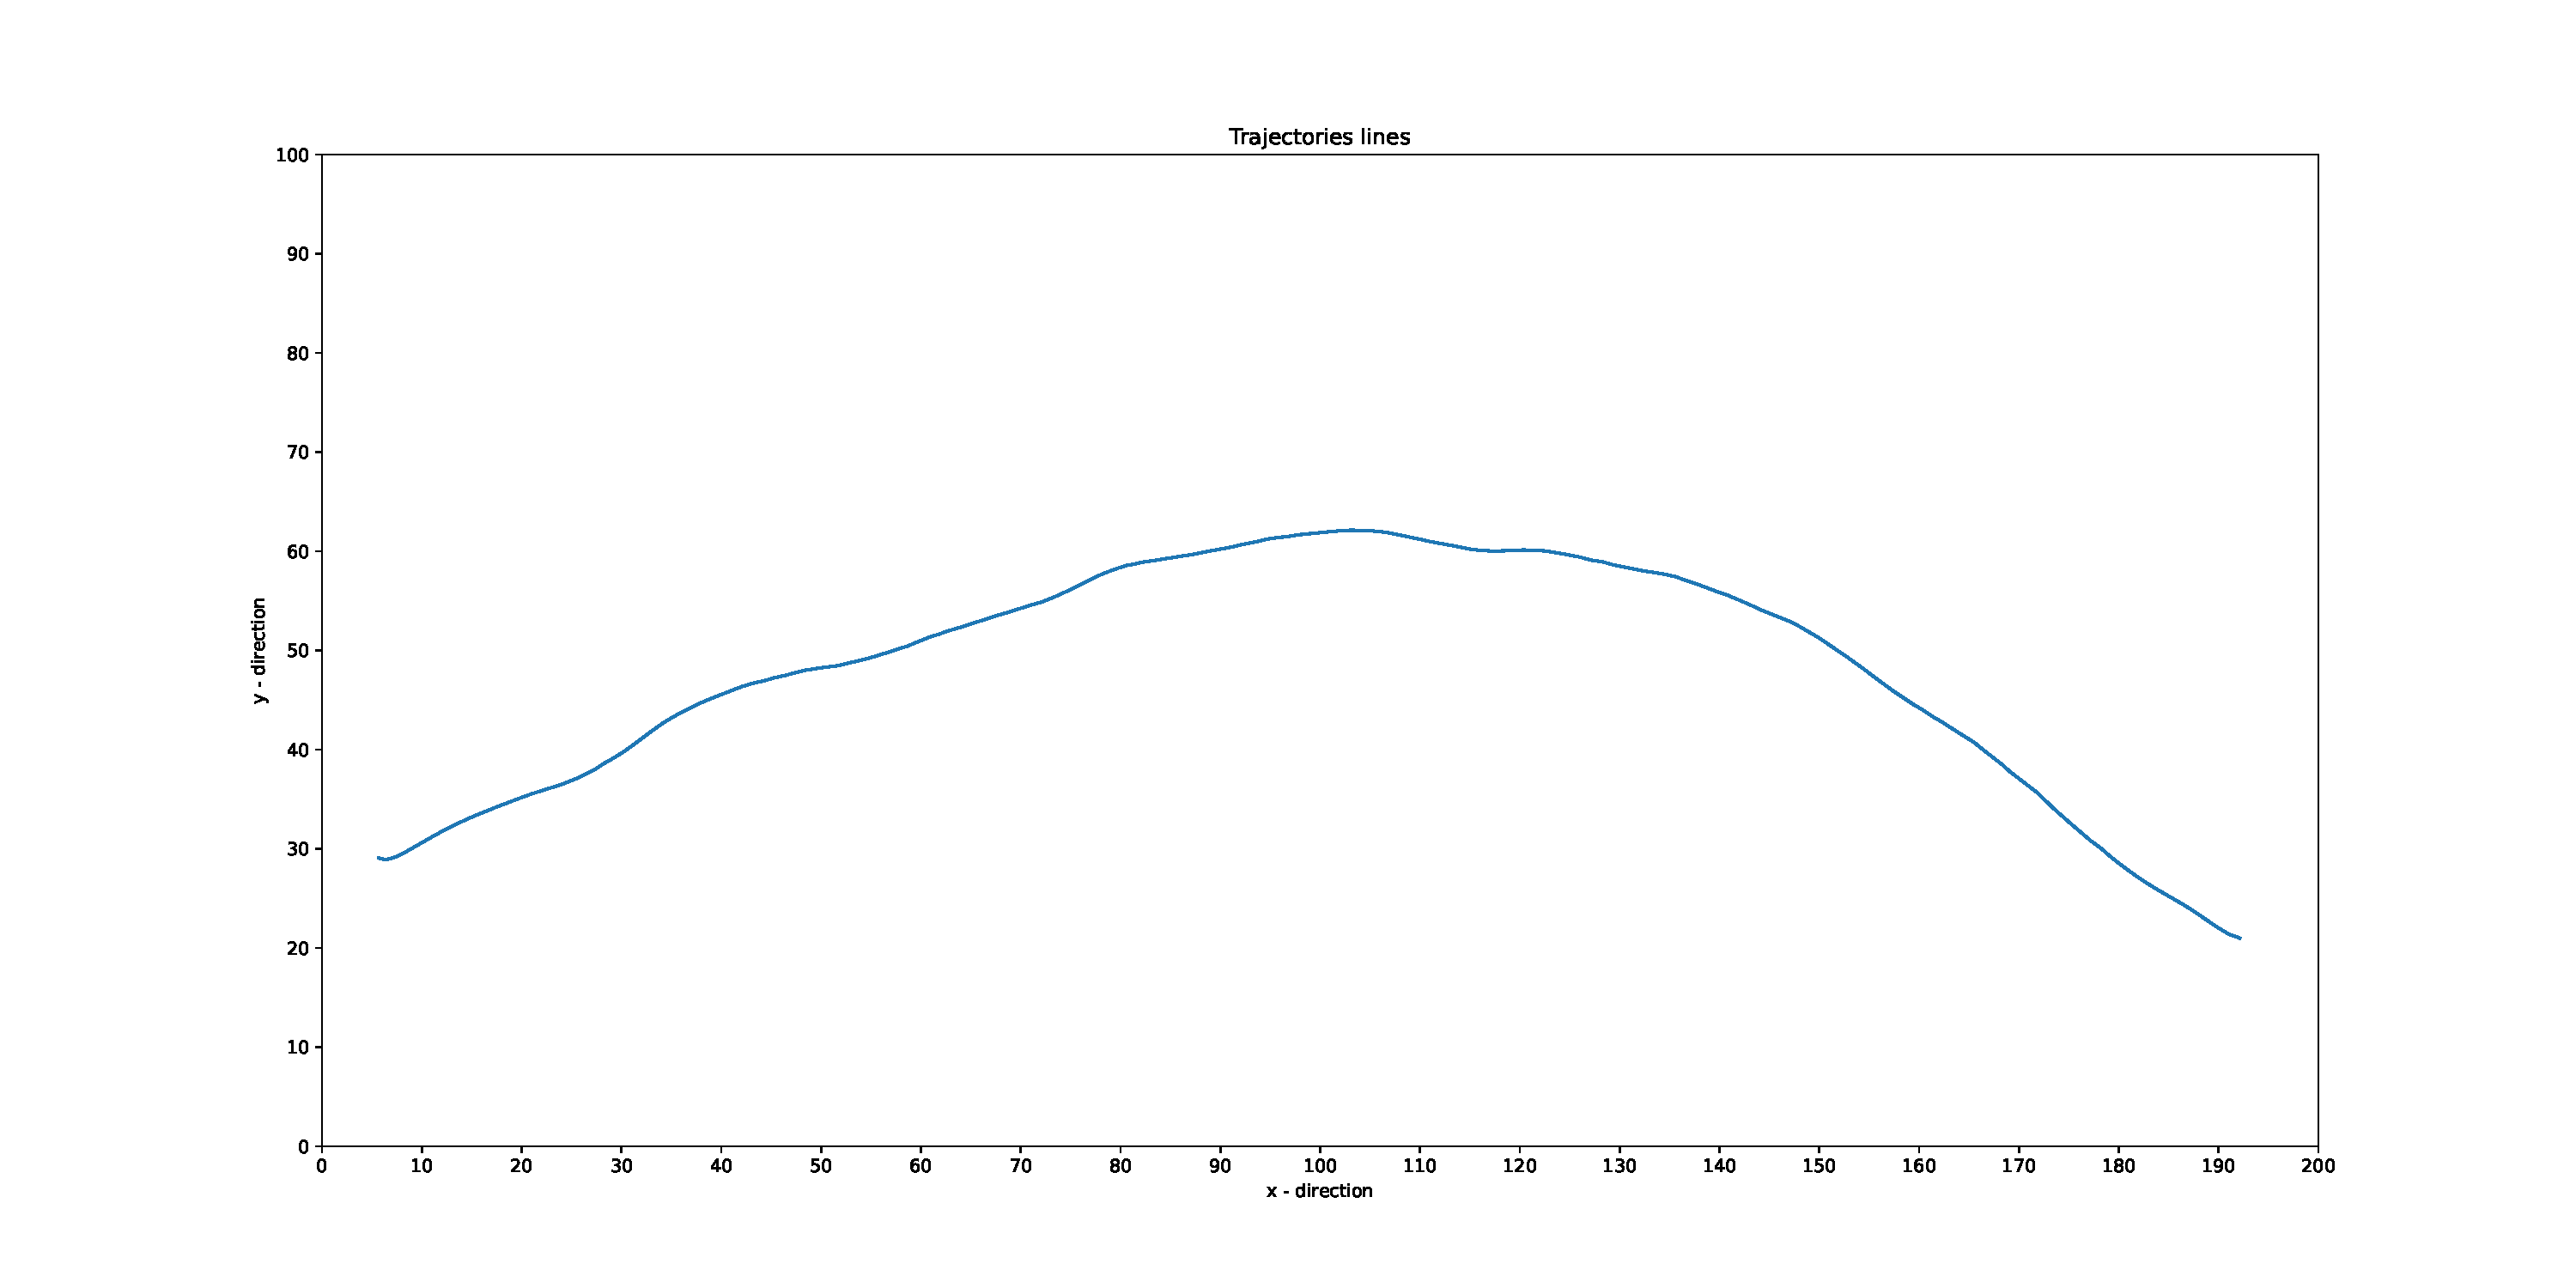
\includegraphics[ width=1\textwidth]{fig/belle_traiettorie/nice selection/figure_trainf10_RealData_lines_19marzo_select_single_NP_19_13075050}
\captionsetup{width=.8\linewidth}
\caption{Plot L}
\label{fig:stranger_i}
\end{minipage}
\begin{minipage}[c]{0.35\linewidth}
\centering
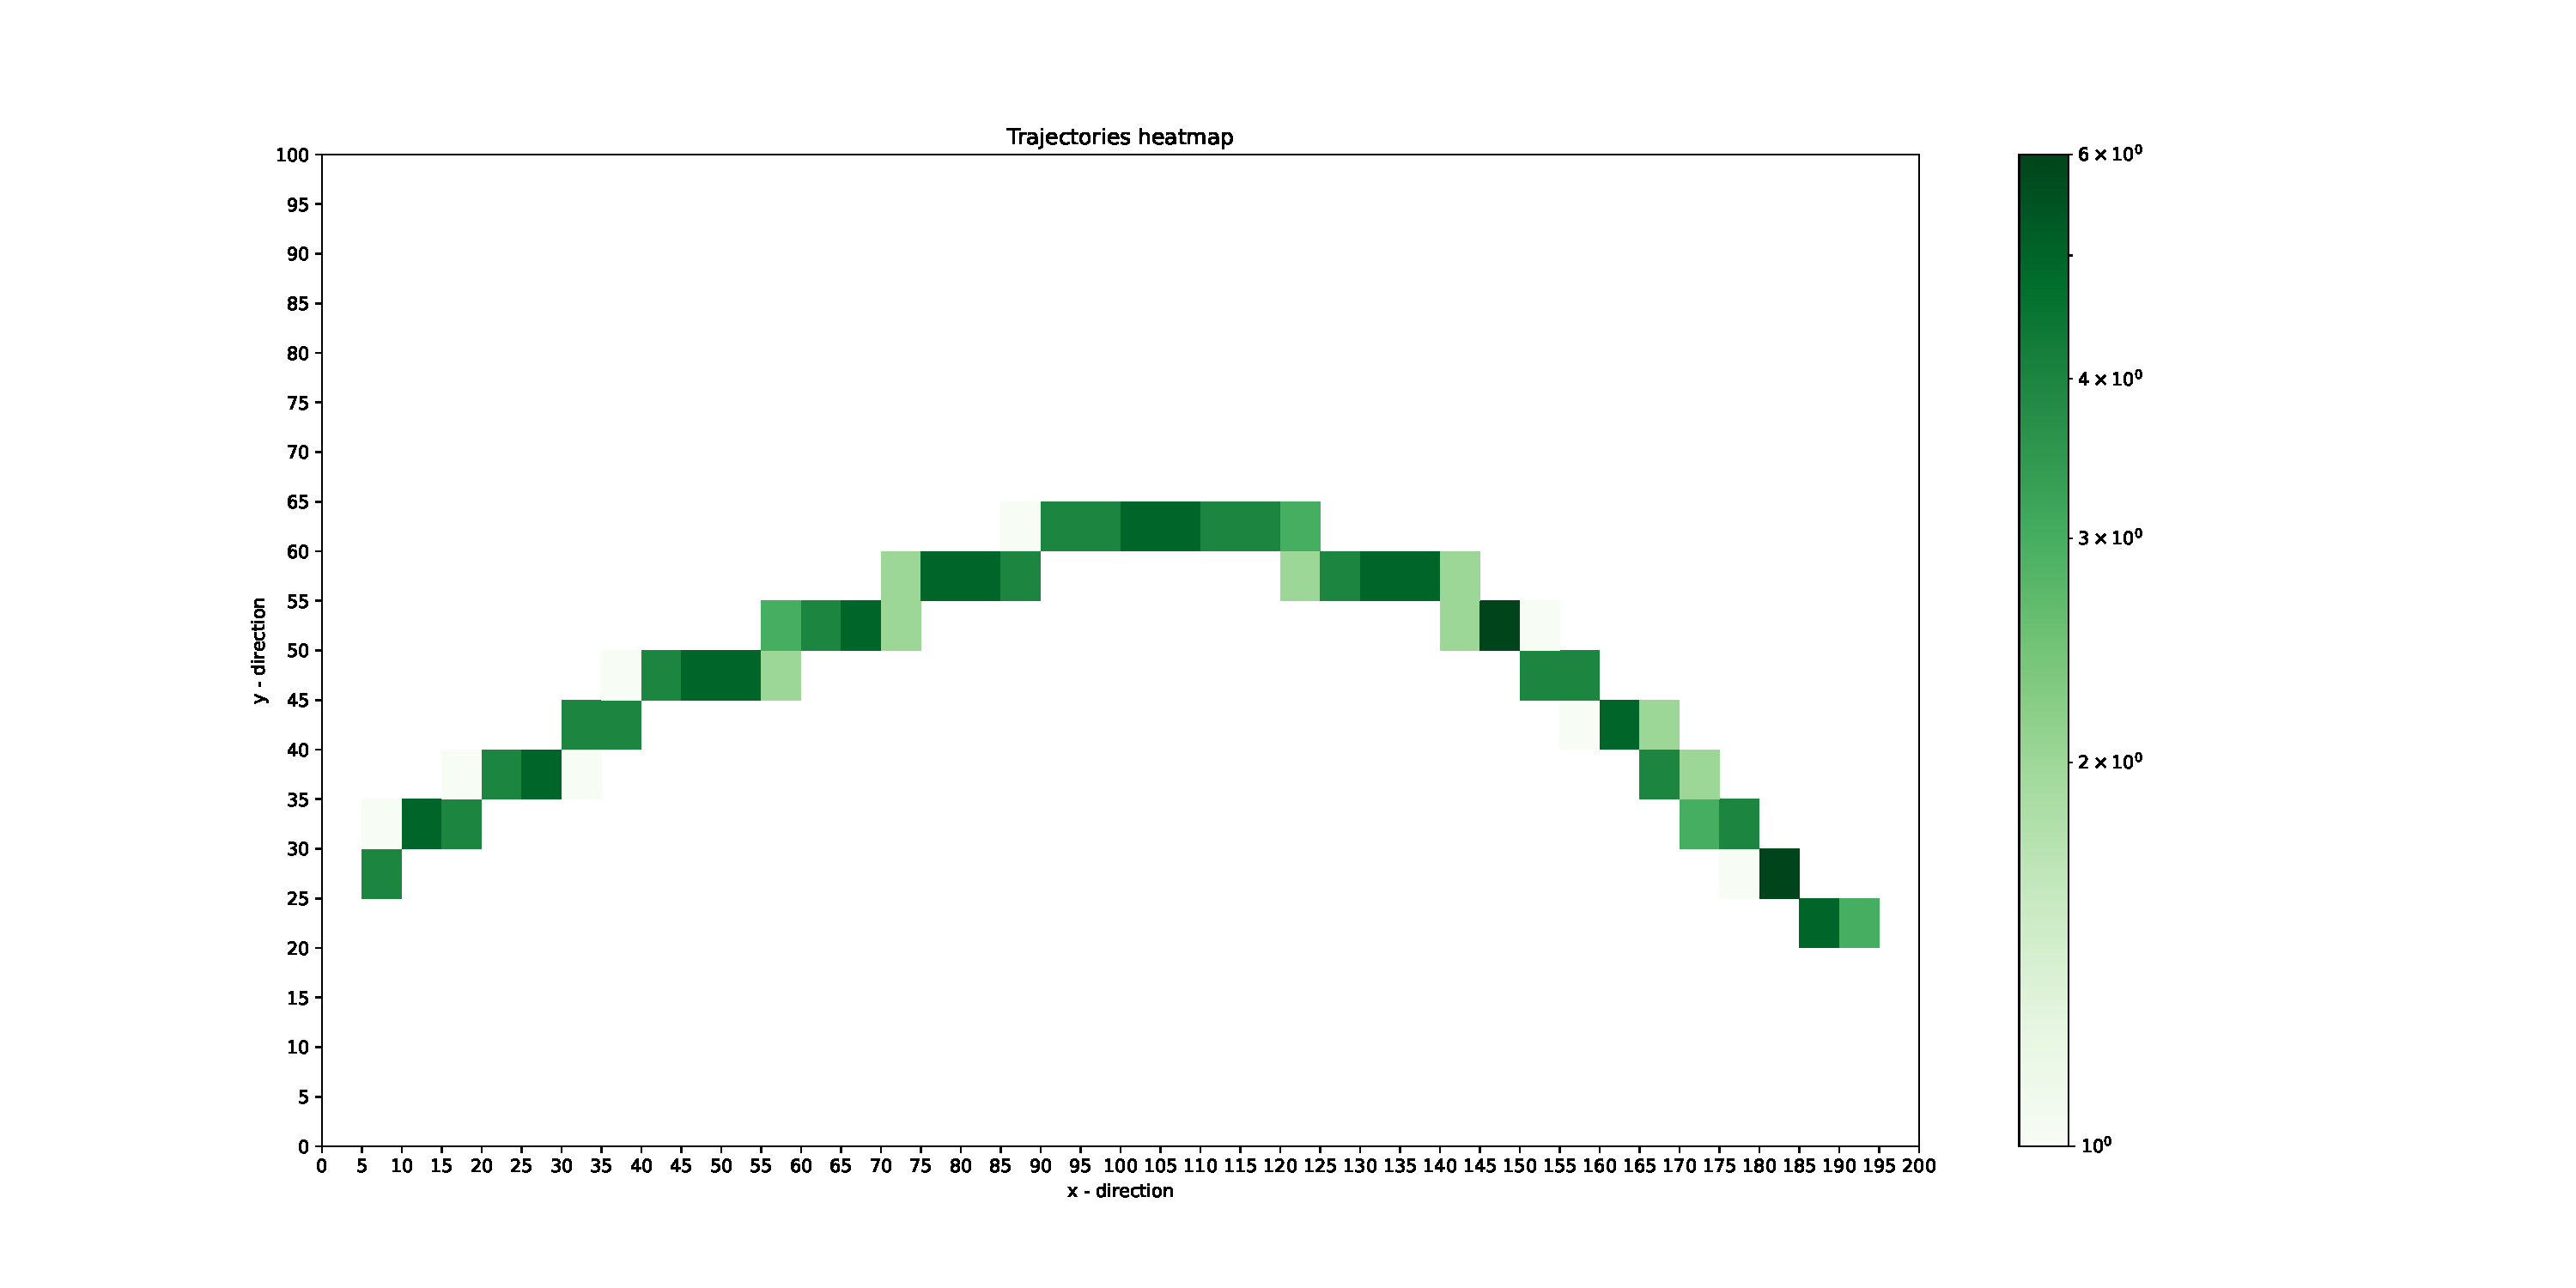
\includegraphics[ width=1\textwidth]{fig/belle_traiettorie/nice selection/figure_trainf10_RealData_heatmap_19marzo_select_single_NP_19_13075050}
\captionsetup{width=.8\linewidth}
\caption{Plot H}
%\label{fig:stranger_i}
\end{minipage}
\begin{minipage}[c]{0.25\linewidth}
\centering
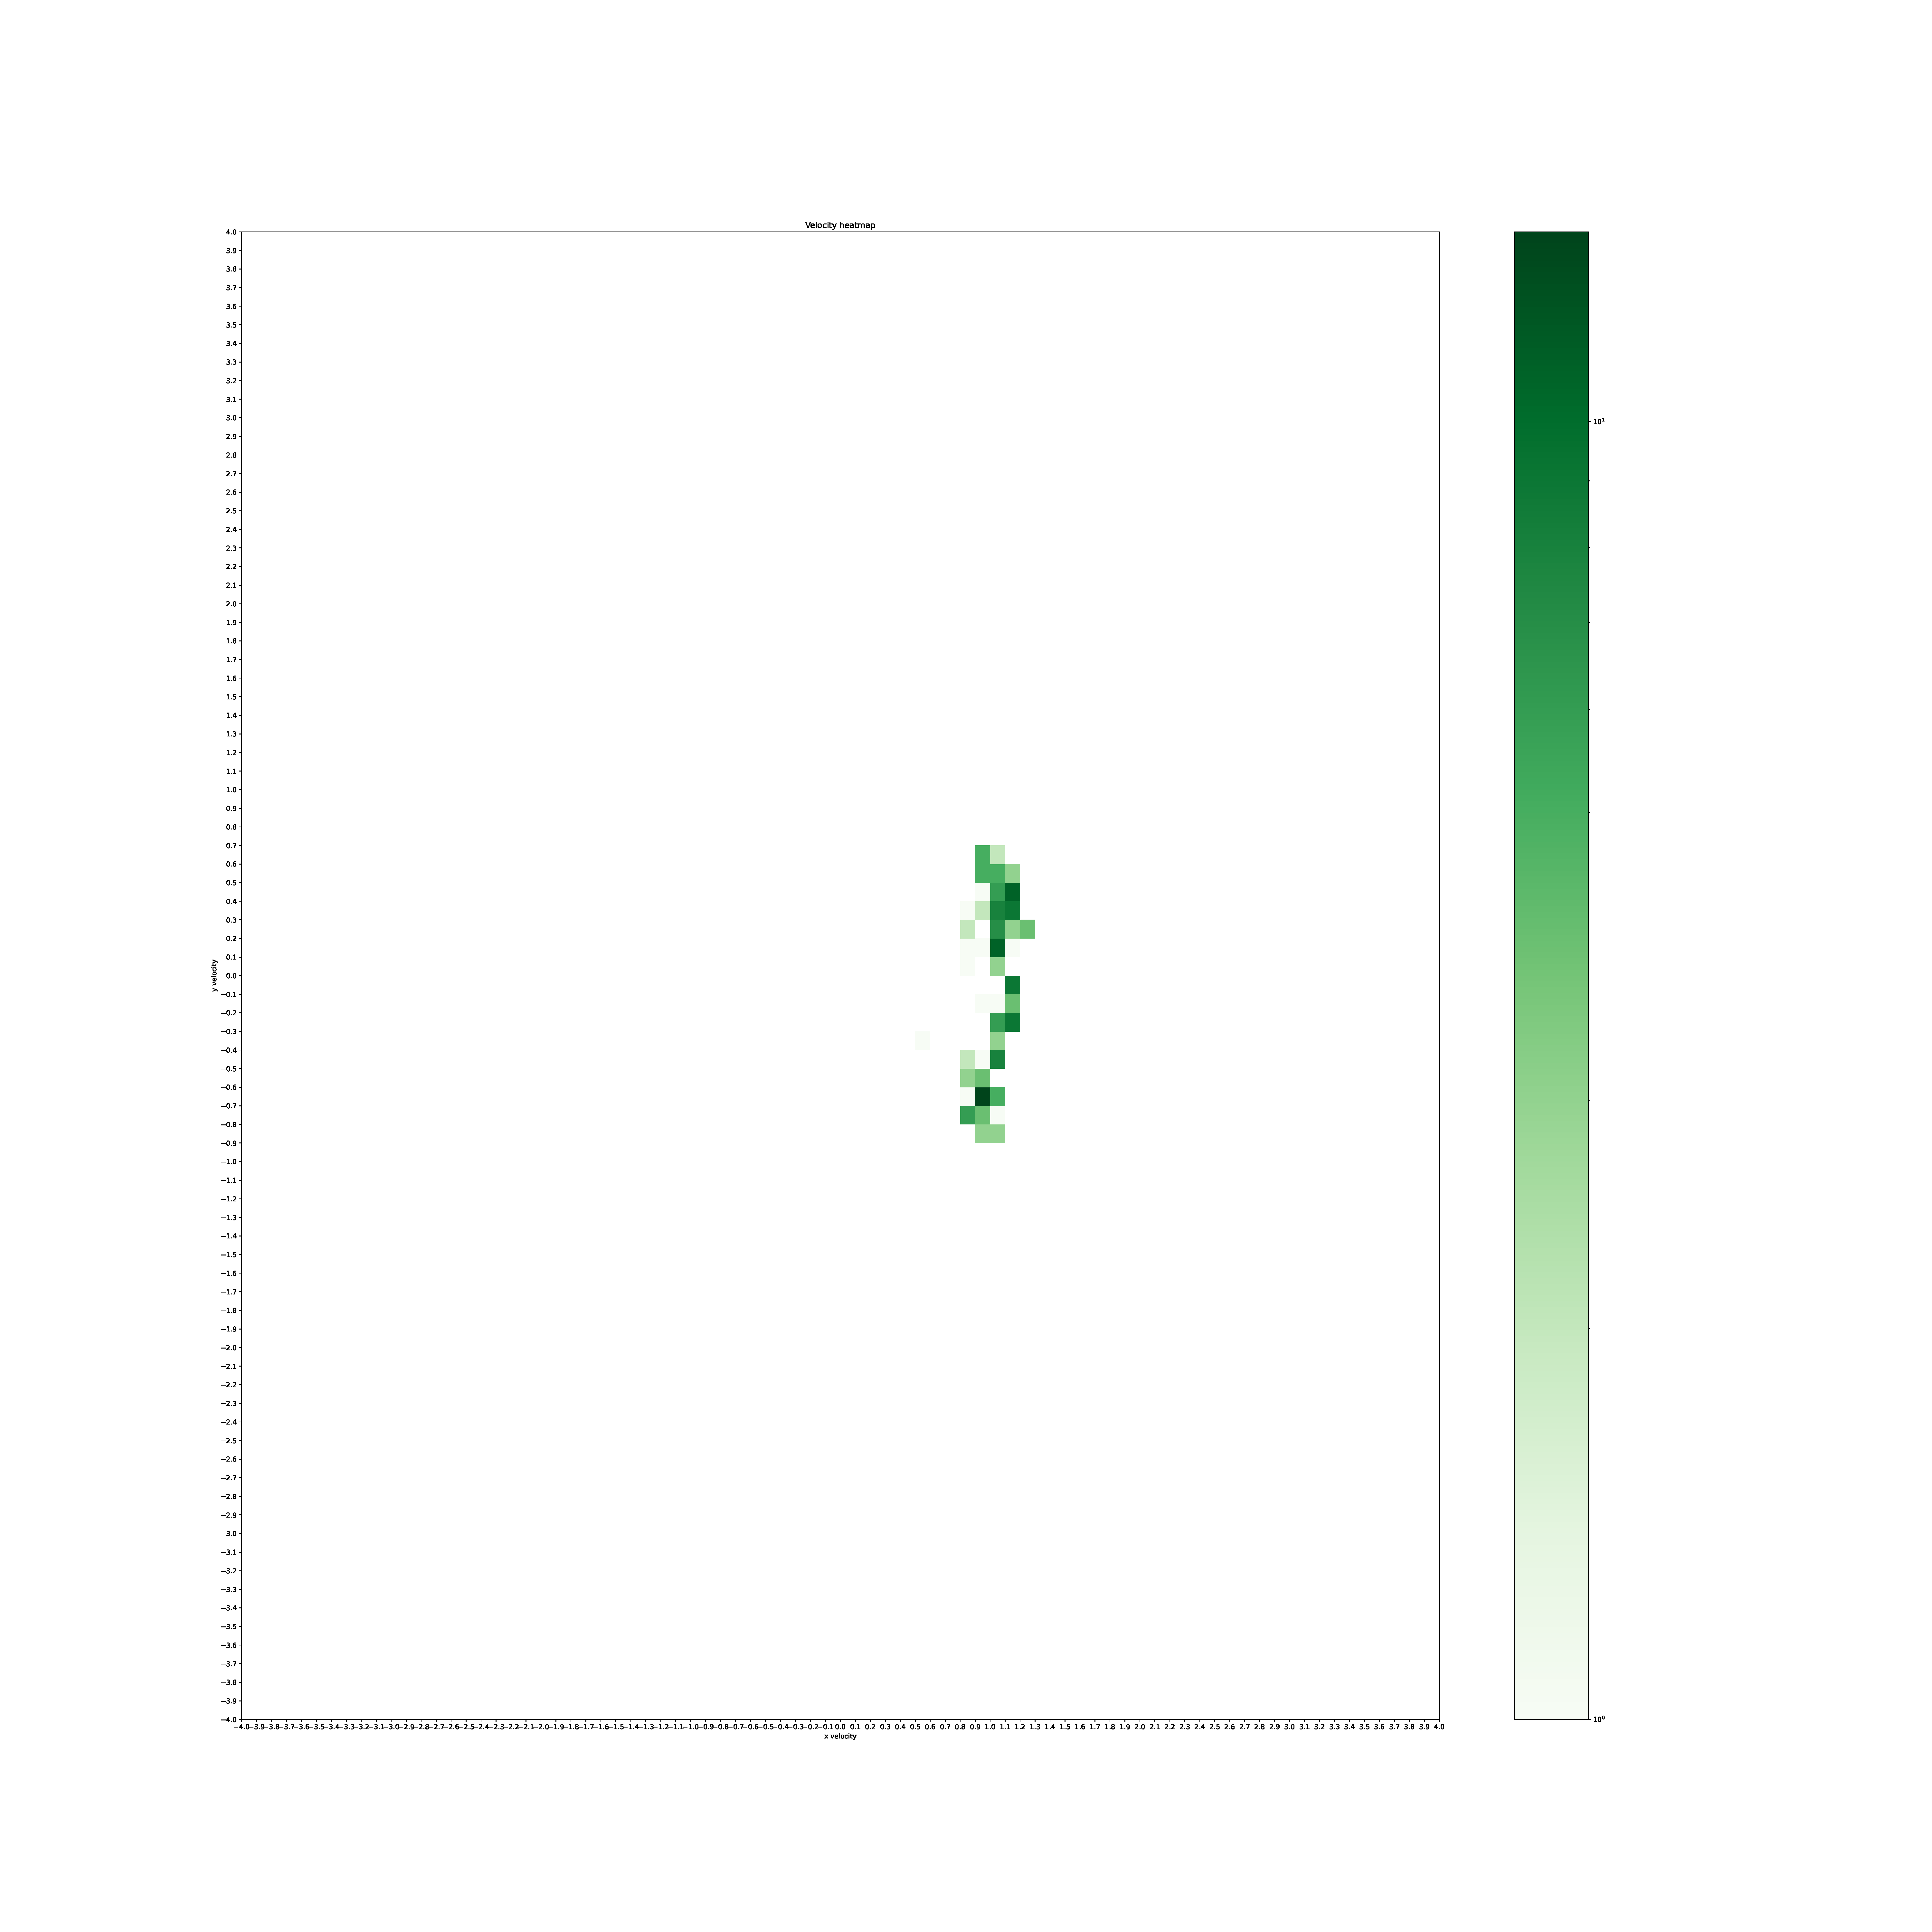
\includegraphics[ width=0.9\textwidth]{fig/belle_traiettorie/nice selection/figure_trainf10_RealData_velocity_heatmap_19marzo_select_single_NP_19_13075050}
\captionsetup{width=.8\linewidth}
\caption{Plot V}
\label{fig:stranger_f}
\end{minipage}
% --- --- --- --- --- --- --- --- --- --- --- --- --- --- --- --- --- --- --- --- --- --- --- --- --- --- --- --- ---
\vspace*{5mm}
\begin{minipage}[c]{0.35\linewidth}
\centering
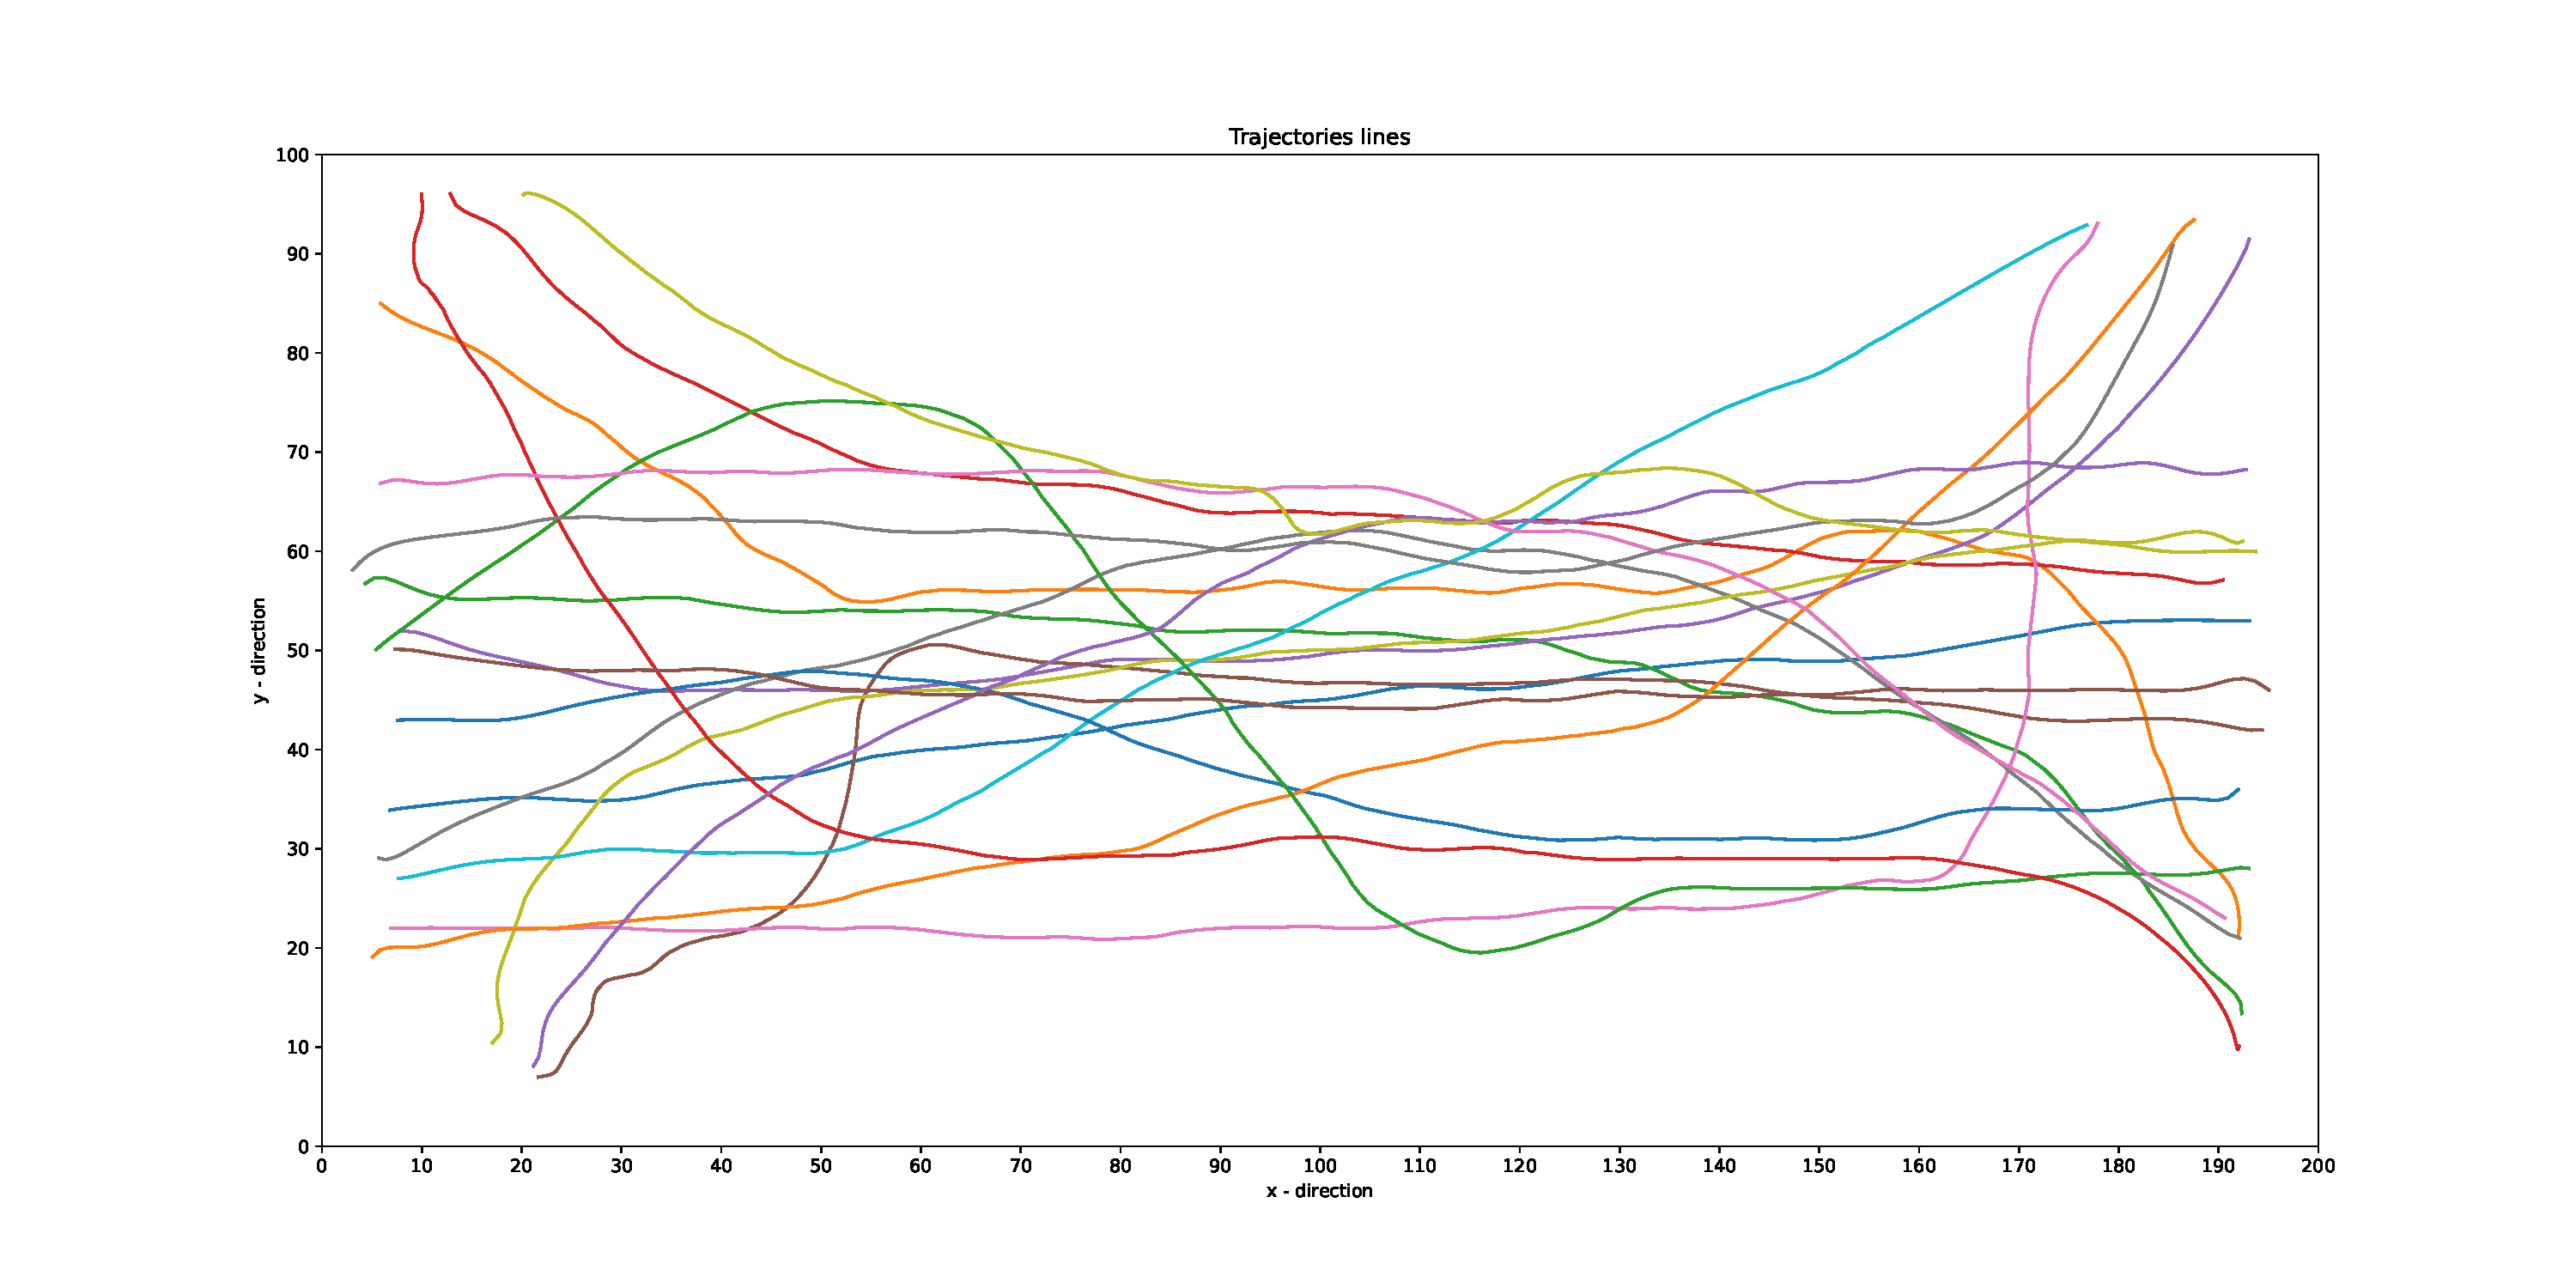
\includegraphics[ width=1\textwidth]{fig/belle_traiettorie/nice selection/figure_trainf10_RealData_lines_19marzo_select_NumP_19_}
\captionsetup{width=.8\linewidth}
\caption{Plot L: \\collection of a few trajectories.}
\label{fig:alltog_i}
\end{minipage} \;
\begin{minipage}[c]{0.35\linewidth}
\centering
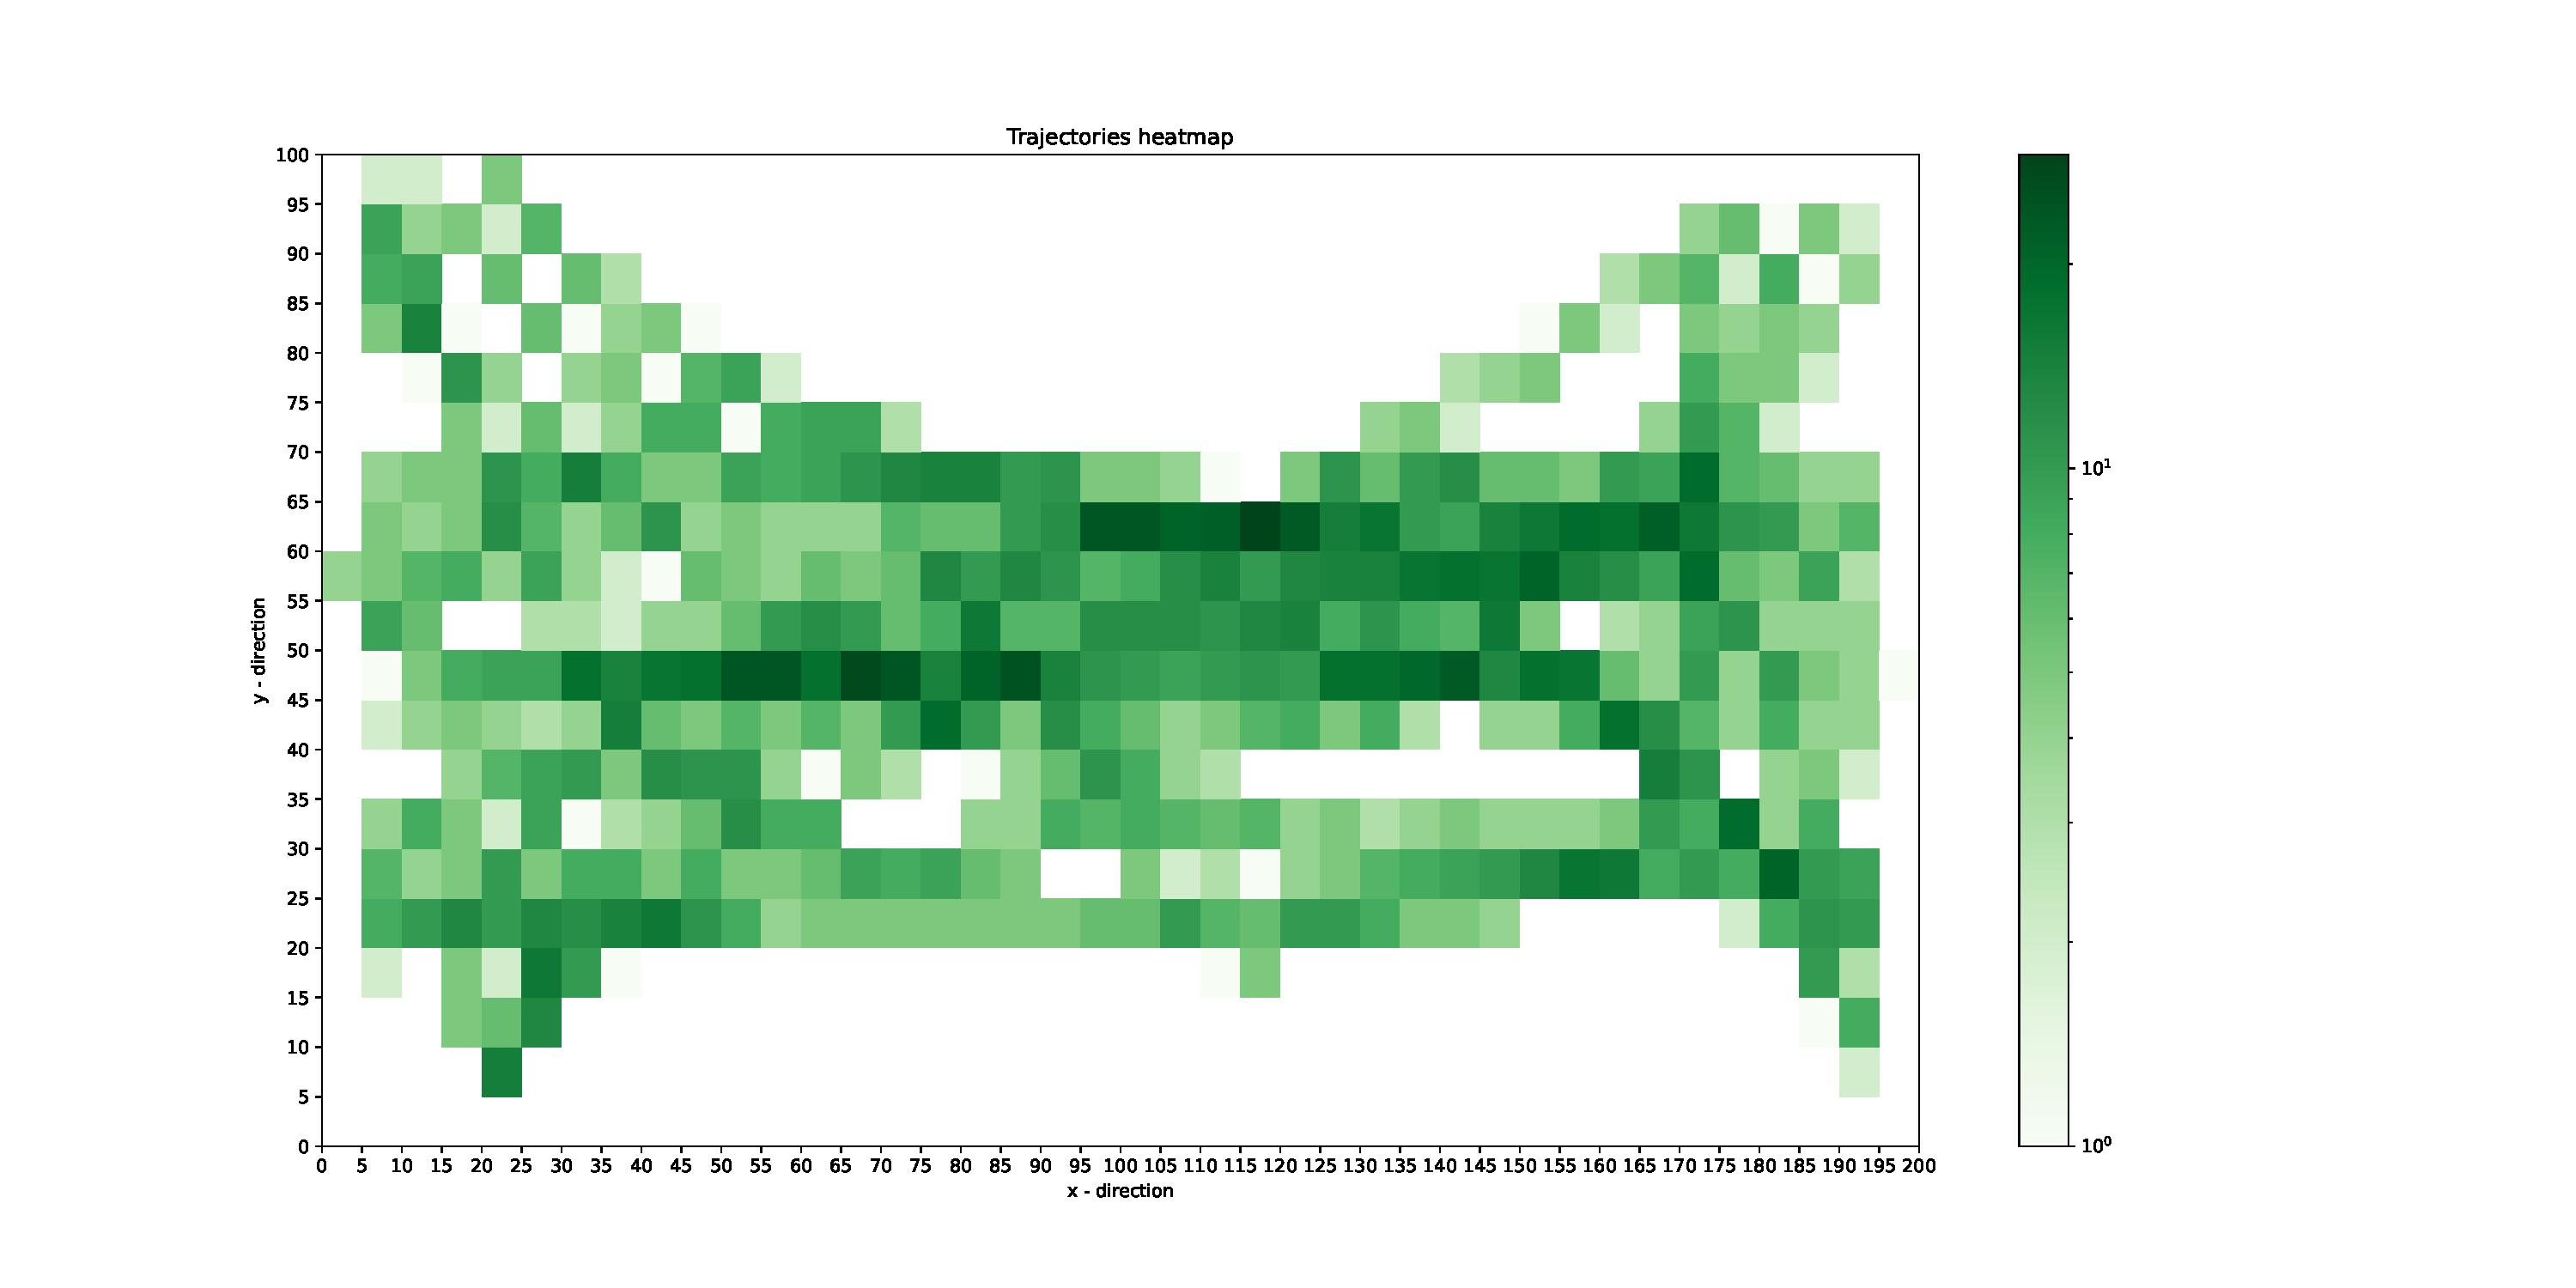
\includegraphics[ width=1\textwidth]{fig/belle_traiettorie/nice selection/figure_trainf10_RealData_heatmap_19marzo_select_NumP_19_}
\captionsetup{width=.8\linewidth}
\caption{Plot H: \\collection of a few trajectories.}
%\label{fig:stranger_i}
\end{minipage} \quad
\begin{minipage}[c]{0.25\linewidth}
\centering
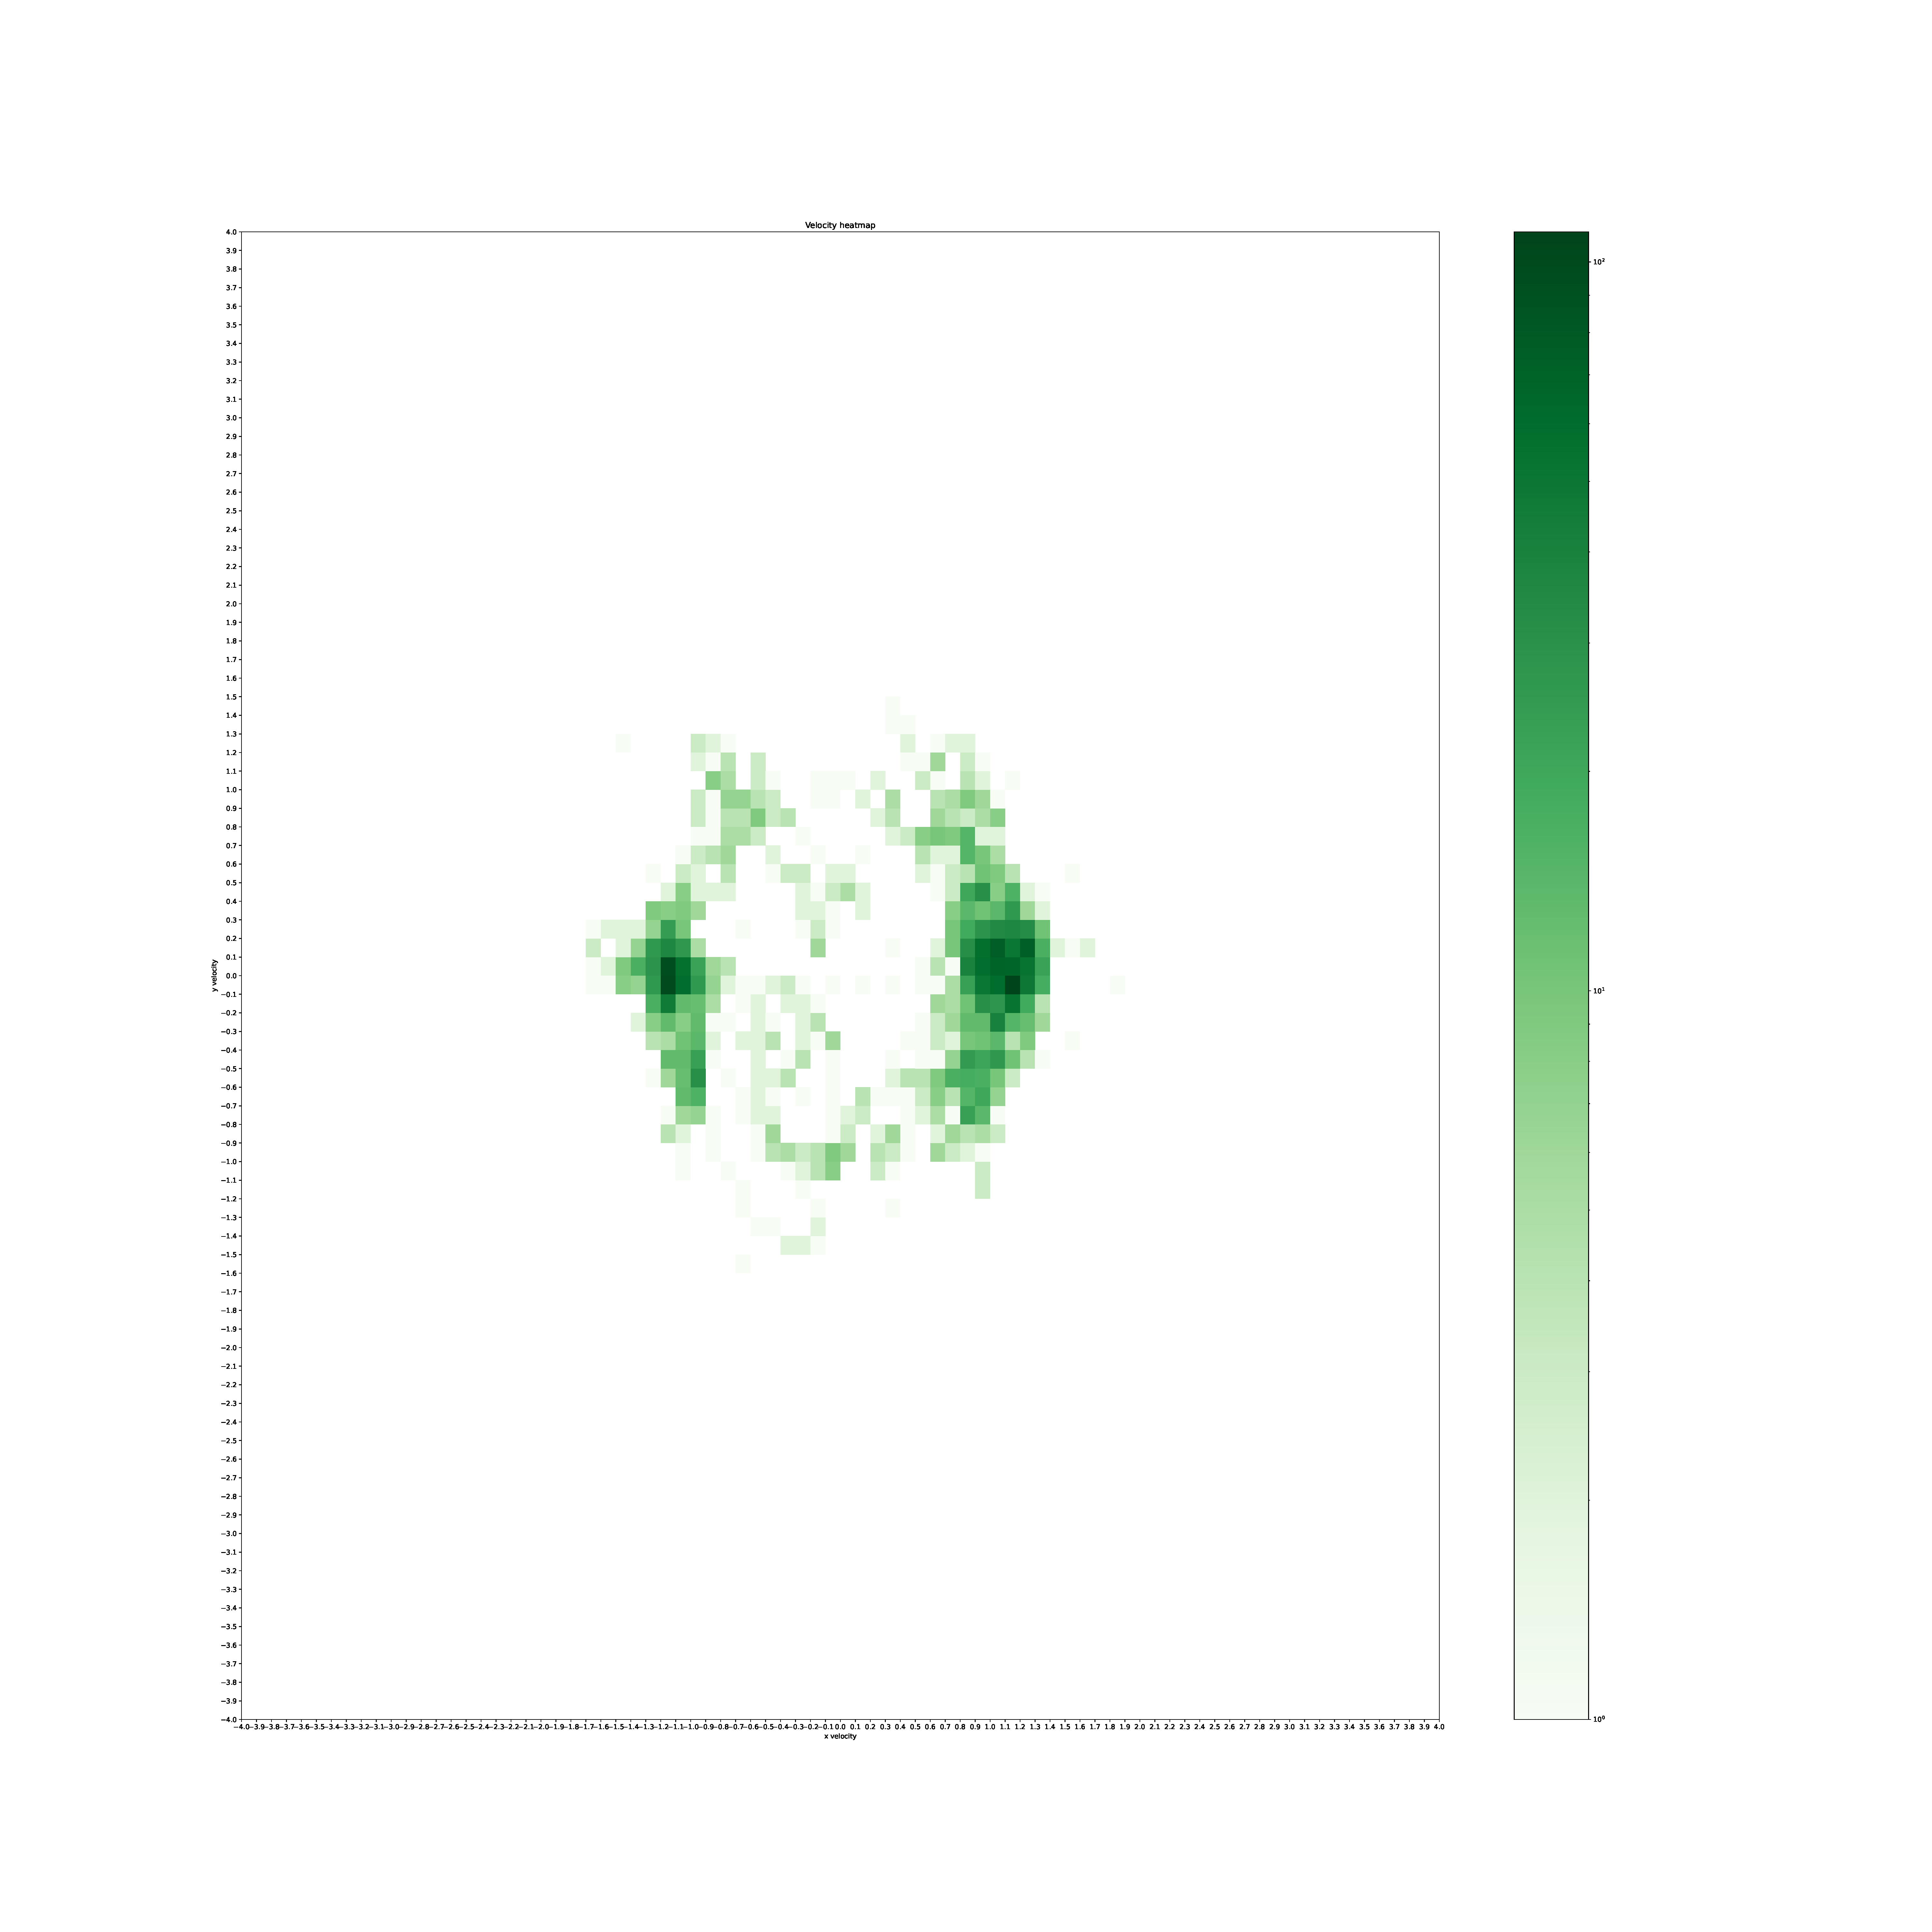
\includegraphics[ width=0.9\textwidth]{fig/belle_traiettorie/nice selection/figure_trainf10_RealData_velocity_heatmap_19marzo_select_NumP_19_}
\captionsetup{width=.8\linewidth}
\caption{Plot V: \\collection of a few trajectories.}
\label{fig:alltog_f}
\end{minipage}
\end{figure}





















\end{document}